\documentclass[a4paper, 12pt]{article}

% Título, autor y fecha
\title{Adogption}
\date{2024-05-10}
\author{Laura Vega Palacios}

% Paquetes
\usepackage[utf8]{inputenc}
\usepackage{subcaption}
\usepackage[table]{xcolor} % Cargado una sola vez
\usepackage{caption}
\usepackage{float}
\usepackage{graphicx} % Cargado una sola vez
\usepackage{epsfig}
\usepackage{multirow}
\usepackage{colortbl}
\usepackage{array} 
\usepackage[parfill]{parskip}
\setlength{\parindent}{30pt}
\usepackage{imakeidx}
\makeindex[columns=3, title=Indice]
\usepackage{hyperref}
\hypersetup{
    colorlinks=true,
    linkcolor=blue,
    filecolor=magenta,      
    urlcolor=cyan,
    pdftitle={Adogption},
    pdfpagemode=FullScreen,
}
\usepackage{geometry}
\usepackage{enumitem}
\usepackage{tocloft}

% Setup
\setcounter{section}{0}
\providecommand{\keywords}[1]{\textbf{\textit{Palabras clave:}} #1}
\renewcommand{\baselinestretch}{1}
\renewcommand{\contentsname}{Índice}
\renewcommand{\listtablename}{Índice de tablas}
\renewcommand{\listfigurename}{Índice de figuras}
\renewcommand{\figurename}{Figura}
\renewcommand{\tablename}{Tabla}

% Empieza el documento
\begin{document}


% Portada
\begin{titlepage}
	\pagestyle{plain}
	\centering
	{
\includegraphics[width=1\textwidth]{logoUGR.png}\par}
	{\bfseries\LARGE Universidad de Granada \par}
	{\scshape\Large Ingeniería Informática \par}
	\vspace{0.5cm}
	{\itshape\Large Trabajo fin de grado \par}
	{\scshape\Huge Desarrollo de Aplicación Móvil para Adopción Canina \par}
	\vfill
	{\Large Autora \par}
	{\Large Laura Vega Palacios\par}

	{\Large Tutor \par}
	{\Large Juan José Escobar Pérez\par}
	\vfill
	{\Large Junio de 2024 \par}
\end{titlepage} 

% Contra portada
\newpage
\thispagestyle{empty}
\mbox{}

% Resumen
\newpage
\pagestyle{plain}
\section*{Resumen}
A día de hoy, comenzar un proceso de adopción puede ser algo tedioso debido a lo descentralizada que está toda la información relacionada con las protectoras y refugios. Una persona que quiera adoptar algún animal normalmente va a necesitar consultar diversas plataformas o redes para encontrar una protectora cercana o un animal que se adapte a su estilo de vida.

El desarrollo de este \textit{Trabajo de Fin de Grado} tiene como finalidad la planificación y desarrollo de una aplicación móvil que permita la gestión de adopciones, la información de las protectoras y facilite la comunicación entre los adoptantes y las protectoras. En esta aplicación, se podrán dar de alta protectoras o refugios, con sus correspondientes datos y ubicación. Las protectoras o refugios que estén verificadas por los administradores tendrán la capacidad de subir a la plataforma todos los caninos, que aparecerán en las listas de adopción o acogida dependiendo de lo que se haya marcado para cada uno. También se podrán dar de alta usuarios que busquen adoptar o acoger algún can y se incluirán formularios para dar de alta o editar la información de ellos, con distintos apartados para cumplimentar todos los datos requeridos como la descripción, la raza, la edad, el peso, etc. Los usuarios también dispondrán de formularios para darse de alta y editar su información. La aplicación utilizará un sistema de geolocalización para mostrar a los usuarios resultados dentro de la aplicación y su distancia. Estos resultados se podrán ver en un mapa insertado en la misma gracias a la inclusión de barras de búsqueda y filtros rápidos para acotar resultados según los requisitos del usuario. Por otro lado, la aplicación incluirá un sistema de mensajería para facilitar la comunicación tanto entre usuarios y protectoras como con los administradores. Este permitirá el envío de mensajes de texto e imágenes. Se añadirá, además, un sistema de favoritos y la posibilidad de compartir caninos de la aplicación de forma externa a través de un enlace. Finalmente la aplicación contendrá una página de información legal y de contacto a disposición del usuario.

% Pagina en blanco
\newpage
\pagestyle{plain}
\thispagestyle{empty}
\mbox{}

% Abstract
\newpage
\pagestyle{plain}
\section*{Abstract}
Nowadays, starting an adoption process can be tedious due to the decentralized that is the information related to shelters and rescue organizations. A person looking to adopt an animal usually needs to check different platforms to find a nearby shelter or an animal that fits their lifestyle.

The purpose of this \textit{Final Degree Project} is to plan and develop a mobile application that facilitates adoption management, provides information about shelters, and eases communication between adopters and shelters. In this application, shelters or rescue organizations can register with their corresponding data and location. Shelters or rescues verified by administrators will have the ability to upload all the dogs to the platform, which will appear in adoption or foster lists depending on the status marked for each dog. Users looking to adopt or foster a dog can also register, and forms will be included to add or edit their information, with different sections to fill in all required data such as description, breed, age, weight, etc. Users will also have forms to register and edit their information. The application will use a geolocation system to show users results within the application and their distance. These results can be viewed on an embedded map thanks to the inclusion of search bars and quick filters to narrow down results according to the user's requirements. Additionally, the application will include a messaging system to facilitate communication between users and shelters as well as with administrators. This will allow the sending of text messages and images. Furthermore, a favorites system will be added, along with the ability to share dogs from the application externally through a link. Finally, the application will contain a legal information and contact page available to the user.

% Pagina en blanco
\newpage
\thispagestyle{empty}
\mbox{}

% Agradecimientos
\newpage
\section*{Agradecimientos}
\begin{center} 
\vspace*{\fill}
A mis tíos, que me dieron la oportunidad de estudiar y seguir adelante.
\vspace*{\fill}
\end{center} 

% Pagina en blanco
\newpage
\thispagestyle{empty}
\mbox{}
% Pagina en blanco
\newpage
\thispagestyle{empty}
\mbox{}

% Indice
\tableofcontents
\listoftables
\listoffigures

% Pagina en blanco
\newpage
\thispagestyle{empty}
\mbox{}

% Introduccion
\newpage
\section{Introducción}

% Motivación
\subsection{Motivación}
Todos los años, numerosas familias se animan a incluir una mascota en su círculo. Sin embargo, miles de mascotas son a su vez abandonadas por muchas de estas familias en todo el mundo. Existen estudios \cite{affinity} que indican que casi 300.000 perros y gatos fueron recogidos sólo en 2022. Estos datos hacen saltar las alarmas de muchas de las asociaciones que luchan por el bienestar y los derechos de los animales. De todos los animales que son abandonados, muchos permanecen en las calles durante el resto de su vida. Otros son recogidos por las autoridades pertinentes y terminan en protectoras o refugios a la espera de encontrar otra familia. Existen organizaciones sin ánimo de lucro que se encargan de ayudar a muchas de las mascotas que están en las calles. Algunas de estas organizaciones son públicas y subvencionadas por el estado. Para garantizar el bienestar y la protección de los animales, en España se publicó una ley \cite{ley} en la que se tratan principalmente los siguientes puntos:
\begin{itemize}[noitemsep]
\item \textbf{Principios generales}
	\begin{itemize}[noitemsep]
	\item Reconocimiento de los animales como seres dotados de sensibilidad.
	\item Fomento de la adopción en lugar de la compra de animales.
	\item Prohibición de prácticas que causen sufrimiento o estrés innecesario a los animales.
	\item Concienciar acerca del bienestar y respeto animal.
	\end{itemize}
\item \textbf{Responsabilidad y tenencia responsable de animales de compañía}
	\begin{itemize}[noitemsep]
	\item Establecimiento de requisitos mínimos de bienestar, cuidado y alojamiento.
	\item Obligación de identificación y registro de los animales de compañía.
	\item Establecimiento de las obligaciones de los propietarios en cuanto a la tenencia responsable, incluyendo la alimentación, hogar y atención veterinaria.
	\item Prohibición de mantener animales en condiciones inadecuadas o de privarles de cuidados esenciales.
	\end{itemize}
\item \textbf{Cría y comercio de animales}
	\begin{itemize}[noitemsep]
	\item Regulación estricta de la cría y comercio de animales de compañía para evitar la explotación y el maltrato.
	\item Obligación de los criadores y comerciantes de cumplir con requisitos específicos de bienestar animal.
	\item Prohibición de la cría indiscriminada y la venta de animales en tiendas físicas, salvo excepciones debidamente justificadas.
	\end{itemize}
\item \textbf{Concienciación y medidas del estado contra abandonos y abusos}
	\begin{itemize}[noitemsep]
	\item Promoción de la educación, el respeto y protección de los animales.
	\item Campañas de conciencación pública sobre el bienestar animal y la tenencia responsable.
	\item Tipificación de conductas de maltrato y abandono como infracciones administrativas o penales, además del establecimiento de sanciones proporcionales a la gravedad de las infracciones.
	\item Obligación de las administraciones públicas de establecer y mantener refugios y centros de acogida para animales abandonados.
	\item Creación de un registro nacional de animales de compañía y establecimientos relacionados con ellos.
	\end{itemize}
\end{itemize}

Esta ley ha sido un avance muy significativo en la legislación española en materia de protección animal, ayudando a crear un entorno más respetuoso y justo para los animales.

A pesar de que la compra de animales en España es legal, muchas organizaciones de bienestar animal y de los derechos de los animales recomiendan optar por la adopción en lugar de la compra. Esta recomendación tiene su origen en lo habitual que es encontrar criaderos donde los animales no disponen de las condiciones necesarias para vivir adecuadamente. Algunos de estos criaderos carecen de cuidados veterinarios, de una alimentación adecuada y de higiene. En algunos artículos \cite{petalatino} podemos encontrar más información sobre esta problemática. Si se opta finalmente por la compra, se recomienda visitar los criaderos a los que se va a comprar el animal para poder garantizar que no se están fomentando criaderos ilegales y que cumplen con las ley de bienestar animal.


Cuando se opta por la adopción, es necesario cumplir un proceso que puede variar según la organización a la que se acuda. Hay ciertos pasos que son comunes después de escoger una organización:

\begin{itemize}[noitemsep]
\item \textbf{Elección del animal:} en este paso, se deberán tener en cuenta las necesidades de la mascota para determinar cuál se adapta mejor al estilo de vida del hogar donde va a residir. Lo habitual en esta etapa es interactuar con diferentes mascotas candidatas a ser adoptadas.
\item \textbf{Solicitud de adopción:} es común que se tenga que cumplimentar un formulario y realizar una entrevista posterior para asegurar que el animal va a ir a un hogar adecuado.
\item \textbf{Evaluación del hogar:} se organiza una visita al hogar donde va a ir el animal para garantizar que el entorno es seguro y adecuado. También se verifica que se disponga de todo lo necesario para recibir a la mascota, como comederos, juguetes, cama, etc.
\item \textbf{Contrato de adopción:} es indispensable para garantizar la protección legal de las mascotas adoptadas. El nuevo dueño debe comprometerse legalmente a proporcionar atención veterinaria y a no abandonar al animal, entre otros puntos. En la mayoría de las organizaciones, es habitual vacunar y colocar un chip al animal antes de que vaya al hogar del nuevo dueño.
\item \textbf{Recogida del animal:} el día de la recogida, se entrega todo el historial médico del animal (si se dispone de él) y la organización suele proporcionar consejos para los nuevos dueños.
\item \textbf{Seguimiento:} se requiere un seguimiento posterior a la adopción para garantizar el bienestar del animal y brindar apoyo o asesoramiento al dueño.
\end{itemize}

Todo este proceso es guiado por la organización correspondiente y es importante completarlo, aunque pueda resultar un poco tedioso. Para iniciar este proceso de adopción, la persona deberá ponerse en contacto previamente con las distintas protectoras o refugios en su área. Esta fase inicial puede presentar diferentes problemas a los adoptantes. En la mayoría de las protectoras, trabajan voluntarios y se sostienen de donaciones, por lo que es común que no cuenten con fondos para generar visibilidad. Muchas protectoras utilizan diversas redes sociales o sus propios sitios web para promocionarse, lo que implica que una persona interesada en adoptar podría tener que utilizar varias plataformas para ponerse en contacto con alguna. A veces, es difícil mantener una comunicación adecuada con diferentes protectoras incluso después de la adopción. Otro problema es que los futuros adoptantes pueden encontrar dificultades al elegir una mascota, ya que la información sobre las diferentes mascotas está dispersa y puede ser una tarea complicada buscar una que cumpla con todos los requisitos del adoptante.

Después de revisar los pasos y los posibles inconvenientes para solicitar un proceso de adopción, se propone una solución en forma de aplicación móvil. Con esta aplicación, se pretende solventar la problemática de la fase inicial de búsqueda de protectoras, proporcionando a los usuarios listas de protectoras cercanas y caninos disponibles, incluyendo filtros para acotar la búsqueda. También se propone como una forma de facilitar a las protectoras la gestión de sus caninos y posibles adoptantes. En definitiva, el objetivo principal de esta aplicación es centralizar la información de las organizaciones y sus mascotas, además de concienciar e incentivar a los usuarios a adoptar.


% Objetivos
\newpage
\subsection{Objetivos del proyecto}

Para satisfacer las necesidades del proyecto propuesto, se han definido una serie de objetivos divididos en dos categorías: los obligatorios, necesarios para garantizar el funcionamiento esperado de la aplicación, y los opcionales, que tienen como propósito añadir funcionalidades adicionales o facilitar su uso.


% Objetivo 1
\begin{table}[H]
	\captionsetup{width=0.95\linewidth}%
   	\captionsetup{singlelinecheck=false}%
	\captionsetup{list=no}%
	\captionsetup{font=bf}
	\captionsetup{labelformat=empty}
	\caption{Objetivo 1}
	\begin{tabular}{ | m{3cm} | m{10cm} | }
		\hline \cellcolor{lightgray}\textbf{Título} & \cellcolor{gray} \textcolor{white}{\textit{Registro de usuarios con diferentes roles}}  \\ \hline
		\cellcolor{lightgray}\textbf{Tipo} & Obligatorio \\ \hline
		\cellcolor{lightgray}\textbf{Descripción} & La aplicación debe ofrecer la opción de registrarse como usuario o como protectora, los formularios correspondientes y almacenando los datos en la base de datos.  \\ \hline
	\end{tabular}
\end{table} 

% Objetivo 2
\begin{table}[H]
	\captionsetup{width=0.95\linewidth}%
   	\captionsetup{singlelinecheck=false}%
	\captionsetup{list=no}%
	\captionsetup{font=bf}
	\captionsetup{labelformat=empty}
	\caption{Objetivo 2}
	\begin{tabular}{ | m{3cm} | m{10cm} | }
		\hline \cellcolor{lightgray}\textbf{Título} & \cellcolor{gray} \textcolor{white}{\textit{Registro de caninos}}  \\ \hline
		\cellcolor{lightgray}\textbf{Tipo} & Obligatorio \\ \hline
		\cellcolor{lightgray}\textbf{Descripción} & La aplicación debe ofrecer la posibilidad de registrar a varios caninos con diferentes características por de las protectoras y almacenar los datos en la base de datos.  \\ \hline
	\end{tabular}
\end{table} 

% Objetivo 3
\begin{table}[H]
	\captionsetup{width=0.95\linewidth}%
   	\captionsetup{singlelinecheck=false}%
	\captionsetup{list=no}%
	\captionsetup{font=bf}
	\captionsetup{labelformat=empty}
	\caption{Objetivo 3}
	\begin{tabular}{ | m{3cm} | m{10cm} | }
		\hline \cellcolor{lightgray}\textbf{Título} & \cellcolor{gray} \textcolor{white}{\textit{Listado de caninos con filtros y búsqueda}}  \\ \hline
		\cellcolor{lightgray}\textbf{Tipo} & Obligatorio \\ \hline
		\cellcolor{lightgray}\textbf{Descripción} & La aplicación debe mostrar diferentes listas de caninos, permitiendo aplicar filtros rápidos y realizar búsquedas. \\ \hline
	\end{tabular}
\end{table} 

% Objetivo 4
\begin{table}[H]
	\captionsetup{width=0.95\linewidth}%
   	\captionsetup{singlelinecheck=false}%
	\captionsetup{list=no}%
	\captionsetup{font=bf}
	\captionsetup{labelformat=empty}
	\caption{Objetivo 4}
	\begin{tabular}{ | m{3cm} | m{10cm} | }
		\hline \cellcolor{lightgray}\textbf{Título} & \cellcolor{gray} \textcolor{white}{\textit{Listado de usuarios con búsqueda}}  \\ \hline
		\cellcolor{lightgray}\textbf{Tipo} & Obligatorio \\ \hline
		\cellcolor{lightgray}\textbf{Descripción} & La aplicación debe mostrar diversas listas de usuarios que permitan realizar búsquedas en ellas.  \\ \hline
	\end{tabular}
\end{table} 

% Objetivo 5
\begin{table}[H]
	\captionsetup{width=0.95\linewidth}%
   	\captionsetup{singlelinecheck=false}%
	\captionsetup{list=no}%
	\captionsetup{font=bf}
	\captionsetup{labelformat=empty}
	\caption{Objetivo 5}
	\begin{tabular}{ | m{3cm} | m{10cm} | }
		\hline \cellcolor{lightgray}\textbf{Título} & \cellcolor{gray} \textcolor{white}{\textit{Inclusión de sección de caninos favoritos}}  \\ \hline
		\cellcolor{lightgray}\textbf{Tipo} & Obligatorio \\ \hline
		\cellcolor{lightgray}\textbf{Descripción} & Se debe incluir un botón de favoritos en los perfiles de los caninos que permita a los usuarios añadir a su sección de favoritos a aquellos que les gusten.  \\ \hline
	\end{tabular}
\end{table} 

% Objetivo 6
\begin{table}[H]
	\captionsetup{width=0.95\linewidth}%
   	\captionsetup{singlelinecheck=false}%
	\captionsetup{list=no}%
	\captionsetup{font=bf}
	\captionsetup{labelformat=empty}
	\caption{Objetivo 6}
	\begin{tabular}{ | m{3cm} | m{10cm} | }
		\hline \cellcolor{lightgray}\textbf{Título} & \cellcolor{gray} \textcolor{white}{\textit{Inclusión de sistema de mensajería entre usuarios}}  \\ \hline
		\cellcolor{lightgray}\textbf{Tipo} & Obligatorio \\ \hline
		\cellcolor{lightgray}\textbf{Descripción} & Se debe permitir a los usuarios abrir un chat con otros usuarios dentro de la aplicación. Además, los usuarios deberán recibir una notificación cuando reciban un mensaje.  \\ \hline
	\end{tabular}
\end{table} 

% Objetivo 7
\begin{table}[H]
	\captionsetup{width=0.95\linewidth}%
   	\captionsetup{singlelinecheck=false}%
	\captionsetup{list=no}%
	\captionsetup{font=bf}
	\captionsetup{labelformat=empty}
	\caption{Objetivo 7}
	\begin{tabular}{ | m{3cm} | m{10cm} | }
		\hline \cellcolor{lightgray}\textbf{Título} & \cellcolor{gray} \textcolor{white}{\textit{Geolocalización y mapas con  resultados}}  \\ \hline
		\cellcolor{lightgray}\textbf{Tipo} & Obligatorio \\ \hline
		\cellcolor{lightgray}\textbf{Descripción} & Se debe incluir la ubicación para ordenar los resultados de la aplicación según la distancia del usuario. Además, se debe agregar una página con un mapa que muestre la ubicación de los resultados junto con una lista de los mismos.  \\ \hline
	\end{tabular}
\end{table} 

% Objetivo 8
\begin{table}[H]
	\captionsetup{width=0.95\linewidth}%
   	\captionsetup{singlelinecheck=false}%
	\captionsetup{list=no}%
	\captionsetup{font=bf}
	\captionsetup{labelformat=empty}
	\caption{Objetivo 8}
	\begin{tabular}{ | m{3cm} | m{10cm} | }
		\hline \cellcolor{lightgray}\textbf{Título} & \cellcolor{gray} \textcolor{white}{\textit{Actualización de datos de caninos}}  \\ \hline
		\cellcolor{lightgray}\textbf{Tipo} & Obligatorio \\ \hline
		\cellcolor{lightgray}\textbf{Descripción} & Se debe permitir actualizar los atributos de los caninos, como el peso, edad, descripción, etc. Además, se debe proporcionar la opción de marcar si está disponible para adoptar/acoger o si ya ha sido adoptado. \\ \hline
	\end{tabular}
\end{table} 

% Objetivo 9
\begin{table}[H]
	\captionsetup{width=0.95\linewidth}%
   	\captionsetup{singlelinecheck=false}%
	\captionsetup{list=no}%
	\captionsetup{font=bf}
	\captionsetup{labelformat=empty}
	\caption{Objetivo 9}
	\begin{tabular}{ | m{3cm} | m{10cm} | }
		\hline \cellcolor{lightgray}\textbf{Título} & \cellcolor{gray} \textcolor{white}{\textit{Actualización de datos de usuarios}}  \\ \hline
		\cellcolor{lightgray}\textbf{Tipo} & Obligatorio \\ \hline
		\cellcolor{lightgray}\textbf{Descripción} & Se debe permitir a un usuario actualizar sus datos personales y sus credenciales. \\ \hline
	\end{tabular}
\end{table} 

% Objetivo 10
\begin{table}[H]
	\captionsetup{width=0.95\linewidth}%
   	\captionsetup{singlelinecheck=false}%
	\captionsetup{list=no}%
	\captionsetup{font=bf}
	\captionsetup{labelformat=empty}
	\caption{Objetivo 10}
	\begin{tabular}{ | m{3cm} | m{10cm} | }
		\hline \cellcolor{lightgray}\textbf{Título} & \cellcolor{gray} \textcolor{white}{\textit{Inclusión de barra de búsqueda de direcciones}}  \\ \hline
		\cellcolor{lightgray}\textbf{Tipo} & Opcional \\ \hline
		\cellcolor{lightgray}\textbf{Descripción} & Posibilidad de que un usuario pueda buscar su dirección y autocompletar automáticamente los diferentes campos del formulario. \\ \hline
	\end{tabular}
\end{table}

% Objetivo 11
\begin{table}[H]
	\captionsetup{width=0.95\linewidth}%
   	\captionsetup{singlelinecheck=false}%
	\captionsetup{list=no}%
	\captionsetup{font=bf}
	\captionsetup{labelformat=empty}
	\caption{Objetivo 11}
	\begin{tabular}{ | m{3cm} | m{10cm} | }
		\hline \cellcolor{lightgray}\textbf{Título} & \cellcolor{gray} \textcolor{white}{\textit{Diseño de tema oscuro}}  \\ \hline
		\cellcolor{lightgray}\textbf{Tipo} & Opcional \\ \hline
		\cellcolor{lightgray}\textbf{Descripción} & Posibilidad de que un usuario pueda cambiar al tema oscuro dentro de la aplicación. \\ \hline
	\end{tabular}
\end{table}  

% Objetivo 12
\begin{table}[H]
	\captionsetup{width=0.95\linewidth}%
   	\captionsetup{singlelinecheck=false}%
	\captionsetup{list=no}%
	\captionsetup{font=bf}
	\captionsetup{labelformat=empty}
	\caption{Objetivo 12}
	\begin{tabular}{ | m{3cm} | m{10cm} | }
		\hline \cellcolor{lightgray}\textbf{Título} & \cellcolor{gray} \textcolor{white}{\textit{Inclusión de un blog}}  \\ \hline
		\cellcolor{lightgray}\textbf{Tipo} & Opcional \\ \hline
		\cellcolor{lightgray}\textbf{Descripción} & Posibilidad de que un usuario pueda añadir publicaciones con imágenes y textos, además de añadir comentarios en las publicaciones para compartir ideas con otros usuarios. \\ \hline
	\end{tabular}
\end{table}  

% Objetivo 13
\begin{table}[H]
	\captionsetup{width=0.95\linewidth}%
   	\captionsetup{singlelinecheck=false}%
	\captionsetup{list=no}%
	\captionsetup{font=bf}
	\captionsetup{labelformat=empty}
	\caption{Objetivo 13}
	\begin{tabular}{ | m{3cm} | m{10cm} | }
		\hline \cellcolor{lightgray}\textbf{Título} & \cellcolor{gray} \textcolor{white}{\textit{Compartición de caninos a través de un enlace}}  \\ \hline
		\cellcolor{lightgray}\textbf{Tipo} & Opcional \\ \hline
		\cellcolor{lightgray}\textbf{Descripción} & Posibilidad de incluir un botón de compartir que permita al usuario generar un enlace al can correspondiente para poder compartirlo a aplicaciones externas. \\ \hline
	\end{tabular}
\end{table}  

% Objetivo 14
\begin{table}[H]
	\captionsetup{width=0.95\linewidth}%
   	\captionsetup{singlelinecheck=false}%
	\captionsetup{list=no}%
	\captionsetup{font=bf}
	\captionsetup{labelformat=empty}
	\caption{Objetivo 14}
	\begin{tabular}{ | m{3cm} | m{10cm} | }
		\hline \cellcolor{lightgray}\textbf{Título} & \cellcolor{gray} \textcolor{white}{\textit{Envío de imágenes dentro del chat}}  \\ \hline
		\cellcolor{lightgray}\textbf{Tipo} & Opcional \\ \hline
		\cellcolor{lightgray}\textbf{Descripción} & Posibilidad de enviar imágenes dentro del chat. \\ \hline
	\end{tabular}
\end{table} 

% Planificación
\newpage
\section{Gestión del proyecto}
\subsection{Planificación temporal}
En esta sección se definen todas las etapas en las que se dividirá el proyecto, los cuales se resumen en un diagrama de Gantt (ver Figura 1). Este diagrama abarca desde enero de 2024 hasta junio del mismo año, estableciendo un marco temporal para cada fase del proyecto y asignando recursos de manera eficiente para alcanzar los objetivos establecidos.

\begin{figure}[H]
	{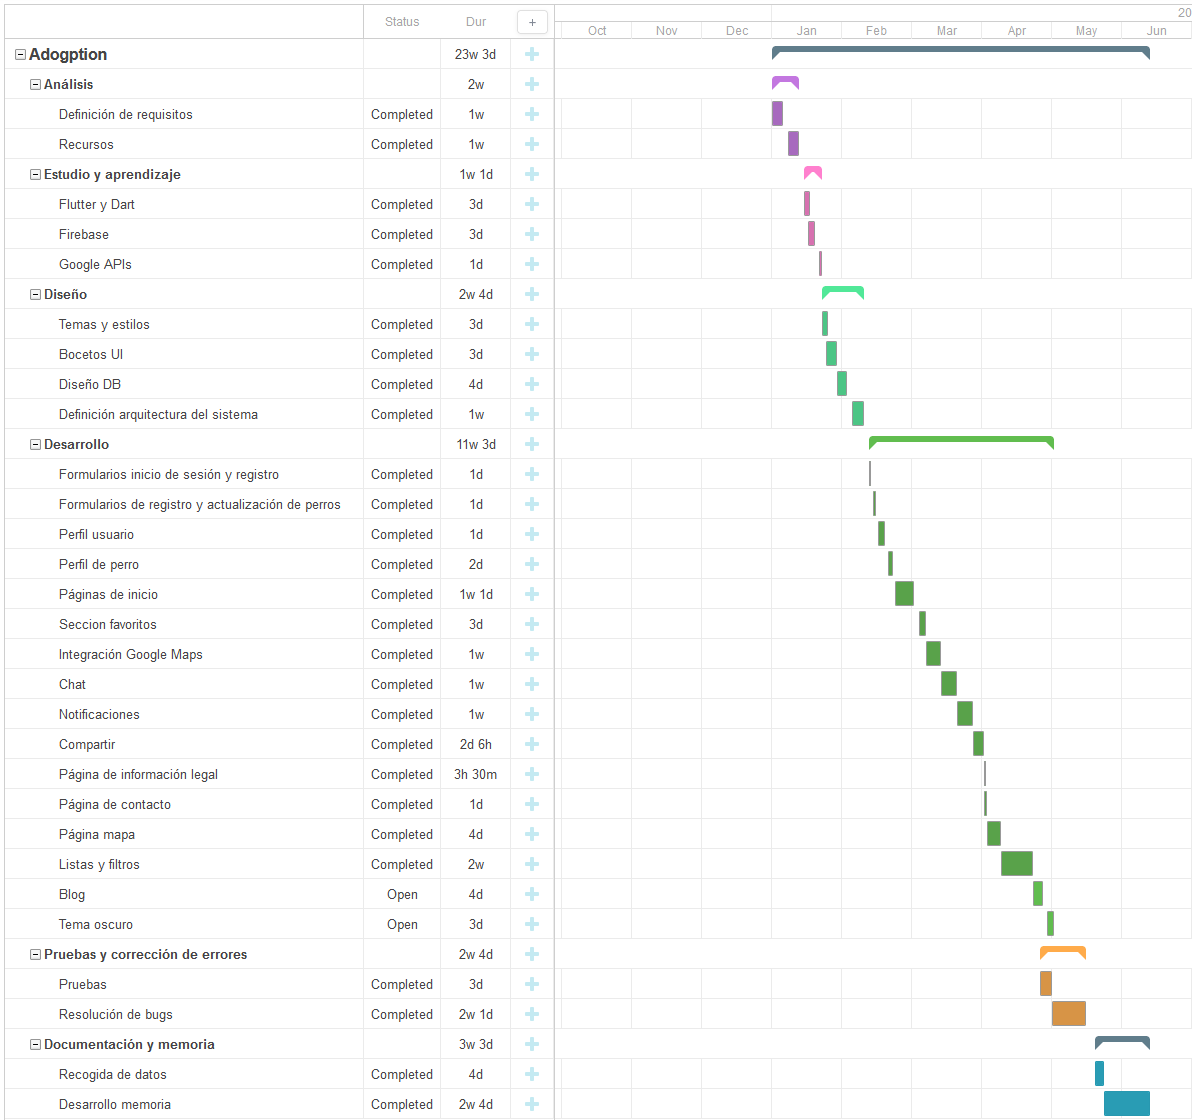
\includegraphics[width=15cm]{diagram/GanntSmall2.png}\par}
	\captionsetup{format=plain,indention=0pt}
	\caption{Diagrama de Gantt.}
	\label{fig:diagramagantt}
\end{figure}

Dentro del diagrama se pueden observar las diferentes etapas del proyecto:

\begin{itemize}[noitemsep]
	\item \textbf{Análisis:} esta etapa tiene una duración aproximada de dos semanas, durante la cual se definen todos los requisitos del sistema y se identifican los recursos humanos, de hardware y de software necesarios.
	\item \textbf{Estudio y aprendizaje:} se asigna un breve período previo para aprender a utilizar los lenguajes y servicios que se emplearán en el desarrollo de la aplicación.
	\item \textbf{Diseño:} se destinan casi tres semanas para definir temas, bocetos, la estructura de la base de datos y la arquitectura del sistema.
	\item \textbf{Desarrollo:} esta es la etapa más extensa, dividida en secciones para cada funcionalidad a desarrollar, a las cuales se les asigna un tiempo adecuado según los servicios y componentes involucrados que definirán su dificultad.
	\item \textbf{Pruebas y corrección de errores:} una vez completado el desarrollo, se realizan pruebas exhaustivas para identificar errores y faltas de funcionalidades. Se reserva tiempo suficiente para corregir errores o implementar mejoras de rendimiento si es necesario.
	\item \textbf{Documentación y memoria:} se dedica un período para recopilar todos los datos y elaborar la memoria en LaTeX, documentando el proceso y los resultados obtenidos en las etapas anteriores.
\end{itemize}

\newpage
\subsection{Estimación de costes}

Para el desarrollo del producto, se puede definir un presupuesto que abarque todos los recursos requeridos.

En este proyecto participará únicamente una persona: la autora de la memoria. Se trata de una ingeniera de software, responsable de todos los aspectos del desarrollo. El horario laboral será de lunes a viernes, a media jornada. Para calcular el costo relacionado con el personal, se ha tomado como referencia el sueldo medio de un programador junior, que ronda los \textit{24.000€} anuales, lo que equivale a \textit{12.000€} a media jornada. Haciendo cálculos, al mes corresponden unos \textit{1.000€}. Dado que la duración del proyecto es de 5 meses y medio, el costo total en salarios para el empleado es de \textit{5.500€}.

Para este proyecto, el hardware disponible incluye un ordenador de sobremesa personal y una tablet Android.

\begin{itemize}[noitemsep]
	\item Ordenador de sobremesa, para el desarrollo y las pruebas, con los siguientes componentes:
		\begin{itemize}[noitemsep]
			\item \textbf{Procesador:} AMD Ryzen 7 3700X 8-Core Processor - 3.60 GHz
			\item \textbf{Memoria RAM:} DDR4 3000 2x16GB
			\item \textbf{Tarjeta gráfica:} NVIDIA GeForce GTX 1660 SUPER
			\item \textbf{Placa base:} ASUS TUF GAMING B550-PLUS WIFI II
			\item \textbf{Disipador:} Noctua NH-D15
		\end{itemize}
	\item Tablet Android Hi9plus, para realizar pruebas en un dispositivo Android físico.
\end{itemize}

Debido a que el equipo utilizado no es nuevo, se consideran los gastos del equipo teniendo en cuenta que un equipo informático se puede amortizar hasta 8 años. El precio aproximado del ordenador es de unos \textit{1.000€}. Un año tiene 12 meses, lo que resulta en 96 meses en total de amortización, lo que implica que cuesta unos \textit{11€} al mes. Dado que la duración del proyecto es de 5 meses y medio, el costo del ordenador sería de \textit{60,50€} en total. El precio de la tablet es de unos \textit{100€}, así que utilizando los mismos cálculos, el costo de la tablet es de \textit{5,72€} en total.

Con respecto al software, para el alcance de este proyecto y los objetivos que se pretenden alcanzar, al menos durante la primera fase, se ha optado por utilizar las versiones gratuitas del software utilizado, lo que resulta en un coste total de 0€.

\begin{itemize}[noitemsep]
	\item Firebase - Plan Spark - Guía de planes \cite{firebase_plans}
	\item Google APIs - Ofrecen créditos gratuitos de hasta \textit{200€} para cubir los gastos que se generen por el uso de la API. - Precios \cite{google_prices}
	\item IDE + Framework - Gratuitos
\end{itemize}


\begin{table}[H]
    \centering
    \begin{tabular}{ | m{5cm} | m{5cm} | m{5cm} | }
	    \hline \textbf{Tipo de recurso} & \textbf{Recurso} & \textbf{Coste (€)} \\ \hline
	    	Personal & Sueldo empleada & 5.500 \\ \hline
		Hardware & Ordenador & 60,50 \\ \hline
		Hardware & Tablet & 5,72 \\ \hline
	    	Software & Firebase & 0 \\ \hline
		Software & Google APIs & 0 \\ \hline
		Software & IDE + Framework & 0 \\ \hline
	   	- & -  & \textbf{Total: 5.566,22€} \\ \hline
    \end{tabular}
    \caption{Costes del proyecto}
    \label{tab:costes}
\end{table}

% Estado del arte
\newpage
\section{Estado del arte}

Hoy en día, la tecnología desempeña un papel fundamental para ayudar a las personas a encontrar protectoras o mascotas para adoptar. Existen diferentes aplicaciones que se centran en las adopciones de caninos u otras mascotas que se utilizan en España, algunas han servido como inspiración durante el desarrollo de \textit{Adogption}. A continuación se incluyen algunas aplicaciones gratuitas que recomienda \textit{La Vanguardia} \cite{lavanguardia}: 

\subsubsection*{Miwuki Pet Shelter}

\textit{Miwuki Pet Shelter} es una plataforma dedicada a la adopción de una amplia variedad de mascotas, incluyendo perros, gatos, roedores, aves, entre otros. Su principal objetivo es facilitar la conexión entre refugios de animales y potenciales adoptantes. La plataforma permite a los refugios crear perfiles detallados de los animales disponibles, proporcionando información exhaustiva sobre su salud, comportamiento y necesidades específicas. Los usuarios pueden explorar la plataforma utilizando filtros avanzados para encontrar mascotas que se adapten a sus preferencias y condiciones de vida. Además de facilitar la adopción, Miwuki promueve activamente la responsabilidad animal mediante recursos educativos sobre el cuidado de mascotas, campañas de esterilización y vacunación, así como ofreciendo seguros veterinarios opcionales para cubrir los gastos asociados al cuidado de las mascotas adoptadas \cite{miwuki}.

\subsubsection*{Ventajas}

Ésta destaca por su interfaz intuitiva y sus funciones de búsqueda avanzadas. Además, Miwuki incluye un blog actualizado regularmente donde se comparten noticias y consejos relacionados con el mundo animal. También cuenta con una sección de informes que presenta cifras y estadísticas sobre el abandono de animales en España, proporcionando así una visión más amplia del problema y fomentando la concienciación sobre la adopción \cite{lookerstudio}.

\subsubsection*{Inconvenientes}

La limitación más importante es que su alcance está principalmente centrado en España.

\subsubsection*{KLYGO}
\textit{KLYGO} es una aplicación móvil especializada en la adopción y acogida de gatos y perros. Facilita la conexión entre usuarios interesados en adoptar o acoger mascotas y diversas protectoras de animales. Una de las características destacadas de ésta es su sistema de geolocalización integrado, que permite a los usuarios visualizar en un mapa las protectoras cercanas. Además, la aplicación ofrece un chat en tiempo real que facilita la comunicación directa entre los adoptantes potenciales y las protectoras, agilizando así el proceso de adopción \cite{klygo}.


\subsubsection*{Ventajas}

La ventaja más destacable de \textit{KLYGO} es el sistema de geolocalización antes mencionado. Por otra parte, la amplia red de refugios y asociaciones colaboradoras añaden un gran valor a esta aplicación. Por último, el chat en tiempo real es de gran utilidad para facilitar el contacto instántaneo entre usuarios y protectoras.

\subsubsection*{Inconvenientes}

Uno de los aspectos que algunos usuarios han reportado es lo poco atractiva e intuitiva que es. Además, la información que contienen las mascotas en sus perfiles no es muy clara o específica.

\subsubsection*{AdoptaMe}

Se trata de una aplicación móvil diseñada específicamente para facilitar la adopción de perros y gatos. Su comunidad enfatiza la adopción responsable, promoviendo la importancia de mantener al día las vacunaciones y la esterilización de los animales. La interfaz de AdoptaMe es relativamente simple y permitie a los usuarios navegar por listas de mascotas y aplicar algunos filtros básicos para encontrar animales disponibles para adopción \cite{adoptame}.

\subsubsection*{Ventajas}

Entre las ventajas de \textit{AdoptaMe} se destaca su enfoque en la adopción responsable, además de la información detallada que se incluye en los perfiles de las mascotas. Los usuarios pueden recibir notificaciones cuando se suben nuevas mascotas a la aplicación, lo cual facilita estar al tanto de las oportunidades de adopción. Además, la aplicación ofrece opciones de filtrado en las listas de mascotas, permitiendo a los usuarios encontrar rápidamente animales que se ajusten a sus criterios específicos.

\subsubsection*{Inconvenientes}

Una posible limitación de Amazdog es su alcance geográfico, que podría estar restringido a ciertas regiones o países específicos, limitando así su accesibilidad para usuarios fuera de esas áreas. Además, aunque la aplicación ofrece perfiles detallados, algunos usuarios podrían desear más opciones de filtrado o clasificación para navegar más eficientemente por las mascotas disponibles.


\subsubsection*{Amazdog}

Una de las aplicaciones más llamativas del mercado es \textit{Amazdog} \cite{amazdog}.

\subsubsection*{Ventajas}


\subsubsection*{Inconvenientes}




% Análisis
\newpage
\section{Análisis de requisitos}

% Definición y Especificación de Requisitos
\subsection{Definición y especificación de requisitos}

En esta sección se detallan los requisitos identificados para la aplicación que se desarrollará. Es fundamental definir y comprender estos requisitos para asegurar resultados óptimos en el desarrollo y diseño del sistema.

\subsubsection{Requisitos funcionales}

Los Requisitos Funcionales (RF) describen las acciones específicas que el sistema debe realizar, los servicios que debe proporcionar y cómo debe responder a diversas entradas. Estos requisitos se centran en el ``qué'' del sistema, delineando las funcionalidades clave que los usuarios esperan encontrar en la aplicación.

% RF1
\begin{table}[H]
\captionsetup{list=no}%
\captionsetup{justification=raggedright,singlelinecheck=false}
\captionsetup{labelformat=empty}
\caption{\textbf{RF1:} Registro de usuarios y protectoras.}
\label{tab:RF1}
	\begin{tabular}{|m{5cm}|m{10cm}|}
	\hline
	\textbf{Descripción} & Ofrecer un formulario de registro para usuarios y protectoras. \\ 
	\hline
	\textbf{Datos de Entrada} & Datos ingresados por el usuario en el formulario de registro, incluyendo datos de contacto, correo electrónico y dirección. \\ 
	\hline
	\textbf{Datos de Salida} & Datos del usuario almacenados en la base de datos. \\ 
	\hline
\end{tabular}
\end{table}

% RF2
\begin{table}[H]
\captionsetup{list=no}%
\captionsetup{justification=raggedright,singlelinecheck=false}
\captionsetup{labelformat=empty}
\caption{\textbf{RF2:} Registro de caninos.}
\label{tab:RF2}
	\begin{tabular}{|m{5cm}|m{10cm}|}
	\hline
	\textbf{Descripción} & Ofrecer un formulario de registro para añadir caninos con características específicas. \\ 
	\hline
	\textbf{Datos de Entrada} & Datos ingresados por la protectora, tales como raza, peso, edad, color y descripción. \\ 
	\hline
	\textbf{Datos de Salida} & Datos del canino almacenados en la base de datos, junto al ID de su protectora. \\ 
	\hline
\end{tabular}
\end{table}

% RF3
\begin{table}[H]
\captionsetup{list=no}%
\captionsetup{justification=raggedright,singlelinecheck=false}
\captionsetup{labelformat=empty}
\caption{\textbf{RF3:} Listado de usuarios.}
\label{tab:RF23}
	\begin{tabular}{|m{5cm}|m{10cm}|}
	\hline
	\textbf{Descripción} & Mostrar diferentes listas de usuarios en la aplicación, con filtros predeterminados. \\ 
	\hline
	\textbf{Datos de Entrada} & Ninguno. \\ 
	\hline
	\textbf{Datos de Salida} & Listas de usuarios de la aplicación que cumplen con los filtros.  \\ 
	\hline
\end{tabular}
\end{table}

% RF4
\begin{table}[H]
\captionsetup{list=no}%
\captionsetup{justification=raggedright,singlelinecheck=false}
\captionsetup{labelformat=empty}
\caption{\textbf{RF4:} Listado de caninos.}
\label{tab:RF4}
	\begin{tabular}{|m{5cm}|m{10cm}|}
	\hline
	\textbf{Descripción} & Mostrar diferentes listas de caninos en la aplicación, con filtros predeterminados \\ 
	\hline
	\textbf{Datos de Entrada} & Ninguno. \\ 
	\hline
	\textbf{Datos de Salida} & Listas de caninos de la aplicación que cumplen con los filtros. \\ 
	\hline
\end{tabular}
\end{table}

% RF5
\begin{table}[H]
\captionsetup{list=no}%
\captionsetup{justification=raggedright,singlelinecheck=false}
\captionsetup{labelformat=empty}
\caption{\textbf{RF5:} Filtrado de caninos según sus atributos.}
\label{tab:RF5}
	\begin{tabular}{|m{5cm}|m{10cm}|}
	\hline
	\textbf{Descripción} & Proporcionar diferentes filtros para las listas de los caninos para ofrecer resultados acotados según sus atributos. \\ 
	\hline
	\textbf{Datos de Entrada} & Valores de los filtros proporcionados por el usuario. \\ 
	\hline
	\textbf{Datos de Salida} & Lista de caninos de la aplicación que cumplen con los filtros. \\ 
	\hline
\end{tabular}
\end{table}

% RF6
\begin{table}[H]
\captionsetup{list=no}%
\captionsetup{justification=raggedright,singlelinecheck=false}
\captionsetup{labelformat=empty}
\caption{\textbf{RF6:} Búsqueda en listas de caninos.}
\label{tab:RF6}
	\begin{tabular}{|m{5cm}|m{10cm}|}
	\hline
	\textbf{Descripción} & Filtrar resultados de listas según el texto ingresado en una barra de búsqueda, la búsqueda se realiza en diferentes atributos de los caninos. \\ 
	\hline
	\textbf{Datos de Entrada} & Texto de búsqueda ingresado por el usuario. \\ 
	\hline
	\textbf{Datos de Salida} &  Lista de caninos de la aplicación que cumplen con el criterio de búsqueda en alguno de los campos. \\ 
	\hline
\end{tabular}
\end{table}

% RF7
\begin{table}[H]
\captionsetup{list=no}%
\captionsetup{justification=raggedright,singlelinecheck=false}
\captionsetup{labelformat=empty}
\caption{\textbf{RF7:} Búsqueda en listas de usuarios.}
\label{tab:RF7}
	\begin{tabular}{|m{5cm}|m{10cm}|}
\hline
	\textbf{Descripción} & Filtrar resultados de listas según el texto ingresado en una barra de búsqueda, la búsqueda se realiza en diferentes campos de los usuarios. \\ 
	\hline
	\textbf{Datos de Entrada} & Texto de búsqueda ingresado por el usuario. \\ 
	\hline
	\textbf{Datos de Salida} &  Lista de usuarios de la aplicación que cumplen con el criterio de búsqueda en alguno de los campos. \\ 
	\hline
\end{tabular}
\end{table}

% RF9
\begin{table}[H]
\captionsetup{list=no}%
\captionsetup{justification=raggedright,singlelinecheck=false}
\captionsetup{labelformat=empty}
\caption{\textbf{RF9:} Marcar/desmarcar canino como favorito.}
\label{tab:RF9}
	\begin{tabular}{|m{5cm}|m{10cm}|}
	\hline
	\textbf{Descripción} & Permitir a un usuario o protectora marcar como favorito a un canino. \\ 
	\hline
	\textbf{Datos de Entrada} & Clic del usuario sobre el botón de favoritos. \\ 
	\hline
	\textbf{Datos de Salida} & Datos del canino con la actualización de IDs de usuarios que lo han marcado/desmarcado como favorito.\\ 
	\hline
\end{tabular}
\end{table}

% RF10
\begin{table}[H]
\captionsetup{list=no}%
\captionsetup{justification=raggedright,singlelinecheck=false}
\captionsetup{labelformat=empty}
\caption{\textbf{RF10:} Inclusión sección de caninos favoritos.}
\label{tab:RF10}
	\begin{tabular}{|m{5cm}|m{10cm}|}
	\hline
	\textbf{Descripción} & Muestra una sección de caninos marcados como favoritos en ese momento por el usuario en su página de inicio. \\ 
	\hline
	\textbf{Datos de Entrada} & Ninguno. \\ 
	\hline
	\textbf{Datos de Salida} & Lista horizontal de caninos favoritos en la parte inferiro de la página de inicio de los usuarios. \\ 
	\hline
\end{tabular}
\end{table}

% RF11
\begin{table}[H]
\captionsetup{list=no}%
\captionsetup{justification=raggedright,singlelinecheck=false}
\captionsetup{labelformat=empty}
\caption{\textbf{RF11:} Inclusión sección de adopciones recientes.}
\label{tab:RF11}
	\begin{tabular}{|m{5cm}|m{10cm}|}
	\hline
	\textbf{Descripción} & Muestra un swiper con imágenes de caninos marcados como adoptados recientemente. \\ 
	\hline
	\textbf{Datos de Entrada} & Ninguno. \\ 
	\hline
	\textbf{Datos de Salida} & Swiper con imágenes y nombres de caninos adoptados en la aplicación. \\ 
	\hline
\end{tabular}
\end{table}

% RF12
\begin{table}[H]
\captionsetup{list=no}%
\captionsetup{justification=raggedright,singlelinecheck=false}
\captionsetup{labelformat=empty}
\caption{\textbf{RF12:} Cerrar sesión.}
\label{tab:RF12}
	\begin{tabular}{|m{5cm}|m{10cm}|}
	\hline
	\textbf{Descripción} & Mostrar botón de cerrar sesión en el menú de acciones en la app bar de la aplicación. \\ 
	\hline
	\textbf{Datos de Entrada} & Ninguno. \\ 
	\hline
	\textbf{Datos de Salida} & Mostrar página de inicio de sesión, después de haber eliminado todos los datos relacionados con el usuario iniciado. \\ 
	\hline
\end{tabular}
\end{table}

% RF14
\begin{table}[H]
\captionsetup{list=no}%
\captionsetup{justification=raggedright,singlelinecheck=false}
\captionsetup{labelformat=empty}
\caption{\textbf{RF14:} Inclusión de menú lateral.}
\label{tab:RF14}
	\begin{tabular}{|m{5cm}|m{10cm}|}
	\hline
	\textbf{Descripción} & Mostrar un botón en la app bar que abre el menú lateral. \\ 
	\hline
	\textbf{Datos de Entrada} & Clic en el botón. \\ 
	\hline
	\textbf{Datos de Salida} & Menu lateral con las páginas disponibles para ese usuario. \\ 
	\hline
\end{tabular}
\end{table}

% RF23
\begin{table}[H]
\captionsetup{list=no}%
\captionsetup{justification=raggedright,singlelinecheck=false}
\captionsetup{labelformat=empty}
\caption{\textbf{RF23:} Edición de datos personales y de contacto.}
\label{tab:RF23}
	\begin{tabular}{|m{5cm}|m{10cm}|}
	\hline
	\textbf{Descripción} & Proporcionar formularios de edición para los datos del usuario. \\ 
	\hline
	\textbf{Datos de Entrada} & Datos ingresados por el usuario en el formulario. Puede haber datos sin actualizar. \\ 
	\hline
	\textbf{Datos de Salida} &  Datos del usuario actualizados en la base de datos. \\ 
	\hline
\end{tabular}
\end{table}

% RF24
\begin{table}[H]
\captionsetup{list=no}%
\captionsetup{justification=raggedright,singlelinecheck=false}
\captionsetup{labelformat=empty}
\caption{\textbf{RF24:} Edición de datos de los caninos.}
\label{tab:RF24}
	\begin{tabular}{|m{5cm}|m{10cm}|}
	\hline
	\textbf{Descripción} & Propocionar formularios de edición para los datos de los caninos. \\ 
	\hline
	\textbf{Datos de Entrada} &  Datos ingresados por el usuario en el formulario. Puede haber datos sin actualizar.  \\ 
	\hline
	\textbf{Datos de Salida} &   Datos del canino actualizados en la base de datos. \\ 
	\hline
\end{tabular}
\end{table}

% RF25
\begin{table}[H]
\captionsetup{list=no}%
\captionsetup{justification=raggedright,singlelinecheck=false}
\captionsetup{labelformat=empty}
\caption{\textbf{RF25:} Recuperación de contraseña.}
\label{tab:RF25}
	\begin{tabular}{|m{5cm}|m{10cm}|}
	\hline
	\textbf{Descripción} & Proporcionar formulario para recuperar la contraseña. \\ 
	\hline
	\textbf{Datos de Entrada} & Correo electrónico ingresado por el usuario. \\ 
	\hline
	\textbf{Datos de Salida} & Correo electrónico con las instrucciones de recuperación de contraseña. \\ 
	\hline
\end{tabular}
\end{table}

% RF26
\begin{table}[H]
\captionsetup{list=no}%
\captionsetup{justification=raggedright,singlelinecheck=false}
\captionsetup{labelformat=empty}
\caption{\textbf{RF26:} Acceder a página de perfil de usuario/protectora.}
\label{tab:RF26}
	\begin{tabular}{|m{5cm}|m{10cm}|}
	\hline
	\textbf{Descripción} & Proporcionar una interfaz que condense toda la información de un usuario en una sola página. \\ 
	\hline
	\textbf{Datos de Entrada} & Ninguno. \\ 
	\hline
	\textbf{Datos de Salida} & Datos del usuario correspondiente, incluyendo foto de perfil, correo y los caninos (si los tiene). \\ 
	\hline
\end{tabular}
\end{table}

% RF27
\begin{table}[H]
\captionsetup{list=no}%
\captionsetup{justification=raggedright,singlelinecheck=false}
\captionsetup{labelformat=empty}
\caption{\textbf{RF27:} Acceder a página de perfil de canino.}
\label{tab:RF27}
	\begin{tabular}{|m{5cm}|m{10cm}|}
	\hline
	\textbf{Descripción} & Proporcionar una interfaz que condense toda la información relacionada con un canino en una sola página. \\ 
	\hline
	\textbf{Datos de Entrada} & Ninguno. \\ 
	\hline
	\textbf{Datos de Salida} & Datos del canino correspondiente, incluyendo foto de perfil, características del canino (edad, raza, peso, descripción...). Además de un mapa indicando su ubicación, el bóton de favoritos y de compartir. También incluye el botón de abrir chat. Contendrá los botones de edición si el canino es del usuario que visita el perfil. \\ 
	\hline
\end{tabular}
\end{table}

% RF28
\begin{table}[H]
\captionsetup{list=no}%
\captionsetup{justification=raggedright,singlelinecheck=false}
\captionsetup{labelformat=empty}
\caption{\textbf{RF28:} Compartir caninos a través de enlace.}
\label{tab:RF28}
	\begin{tabular}{|m{5cm}|m{10cm}|}
	\hline
	\textbf{Descripción} & Proporcionar un botón que genere un enlace para redirigir a un usuario al perfil de ese canino en concreto. \\ 
	\hline
	\textbf{Datos de Entrada} & Ninguno. \\ 
	\hline
	\textbf{Datos de Salida} & Url a la aplicación con los parámetros correspondientes para redirigir al perfil de canino. \\ 
	\hline
\end{tabular}
\end{table}

% RF29
\begin{table}[H]
\captionsetup{list=no}%
\captionsetup{justification=raggedright,singlelinecheck=false}
\captionsetup{labelformat=empty}
\caption{\textbf{RF29:} Mostrar resultados de protectoras en un mapa.}
\label{tab:RF29}
	\begin{tabular}{|m{5cm}|m{10cm}|}
	\hline
	\textbf{Descripción} & Proporcionar una interfaz que contenga un mapa con diferentes marcadores para cada una de las protectoras y un listado de las mismas debajo del mapa. \\ 
	\hline
	\textbf{Datos de Entrada} & Ninguno. \\ 
	\hline
	\textbf{Datos de Salida} & Mapa con marcadores y listado de protectoras, con elementos que pueden mover la cámara a los diferentes marcadores del mapa. \\ 
	\hline
\end{tabular}
\end{table}


% RF30
\begin{table}[H]
\captionsetup{list=no}%
\captionsetup{justification=raggedright,singlelinecheck=false}
\captionsetup{labelformat=empty}
\caption{\textbf{RF30:} Listado de chats disponibles.}
\label{tab:RF30}
	\begin{tabular}{|m{5cm}|m{10cm}|}
	\hline
	\textbf{Descripción} & Proporcionar una interfaz que contenga un listado de chats abiertos dentro de la aplicación. \\ 
	\hline
	\textbf{Datos de Entrada} & Ninguno. \\ 
	\hline
	\textbf{Datos de Salida} & Listado de chats disponibles en la aplicación, incluyen una preview del último mensaje y datos del usuario correspondiente. \\ 
	\hline
\end{tabular}
\end{table}


% RF31
\begin{table}[H]
\captionsetup{list=no}%
\captionsetup{justification=raggedright,singlelinecheck=false}
\captionsetup{labelformat=empty}
\caption{\textbf{RF31:} Envío mensajes de texto al chat.}
\label{tab:RF31}
	\begin{tabular}{|m{5cm}|m{10cm}|}
	\hline
	\textbf{Descripción} & Permitir mandar mensajes a otro usuario dentro de la aplicación. \\ 
	\hline
	\textbf{Datos de Entrada} & Texto ingresado por el usuario. \\ 
	\hline
	\textbf{Datos de Salida} & Mensaje guardado en la base de datos Se ctualizar la tabla de chats de la base de datos con el último mensaje enviado y generar el id del chat si es el primer mensaje. Notificación al usuario receptor. \\ 
	\hline
\end{tabular}
\end{table}


% RF32
\begin{table}[H]
\captionsetup{list=no}%
\captionsetup{justification=raggedright,singlelinecheck=false}
\captionsetup{labelformat=empty}
\caption{\textbf{RF32:} Enviar imágenes al chat.}
\label{tab:RF32}
	\begin{tabular}{|m{5cm}|m{10cm}|}
\hline
	\textbf{Descripción} & Permitir mandar mensajes a otro usuario dentro de la aplicación. \\ 
	\hline
	\textbf{Datos de Entrada} & Imagen adjuntada por el usuario. \\ 
	\hline
	\textbf{Datos de Salida} & Imagen guardada además de su referencia en la tabla de mensaje. Se la tabla de chats de la base de datos con el último mensaje enviado y generar el id del chat si es el primer mensaje. Notificación al usuario receptor. \\ 
	\hline
\end{tabular}
\end{table}


% RF33
\begin{table}[H]
\captionsetup{list=no}%
\captionsetup{justification=raggedright,singlelinecheck=false}
\captionsetup{labelformat=empty}
\caption{\textbf{RF33:} Abrir un chat nuevo.}
\label{tab:RF33}
	\begin{tabular}{|m{5cm}|m{10cm}|}
	\hline
	\textbf{Descripción} & Proporcionar un botón de contacto para abrir un chat con algún usuario dentro de la aplicación. \\ 
	\hline
	\textbf{Datos de Entrada} & Ninguno. \\ 
	\hline
	\textbf{Datos de Salida} & Interfaz del chat, con la cabecera que incluye los datos del usuario receptor. \\ 
	\hline
\end{tabular}
\end{table}

% RF34
\begin{table}[H]
\captionsetup{list=no}%
\captionsetup{justification=raggedright,singlelinecheck=false}
\captionsetup{labelformat=empty}
\caption{\textbf{RF34:} Eliminar un chat.}
\label{tab:RF34}
	\begin{tabular}{|m{5cm}|m{10cm}|}
	\hline
	\textbf{Descripción} & Deslizar un chat para eliminarlo de la lista de chats disponibles \\ 
	\hline
	\textbf{Datos de Entrada} & Ninguno. \\ 
	\hline
	\textbf{Datos de Salida} & Lista actualizada sin el chat que se acaba de eliminar \\ 
	\hline
\end{tabular}
\end{table}

% RF35
\begin{table}[H]
\captionsetup{list=no}%
\captionsetup{justification=raggedright,singlelinecheck=false}
\captionsetup{labelformat=empty}
\caption{\textbf{RF35:} Marcar/desmarcar canino como adoptado.}
\label{tab:RF35}
	\begin{tabular}{|m{5cm}|m{10cm}|}
	\hline
	\textbf{Descripción} & Proporcionar un botón dentro del perfil del canino que permite a una protectora marcar/desmarcar a un canino de la aplicación como adoptado. \\ 
	\hline
	\textbf{Datos de Entrada} & Estado nuevo según si se quiere marcar o desmarcar. \\ 
	\hline
	\textbf{Datos de Salida} & Perfil del canino actualizado y una etiqueta que indica si está adoptado. \\ 
	\hline
\end{tabular}
\end{table}


% RF36
\begin{table}[H]
\captionsetup{list=no}%
\captionsetup{justification=raggedright,singlelinecheck=false}
\captionsetup{labelformat=empty}
\caption{\textbf{RF36:} Inclusión información de contacto.}
\label{tab:RF36}
	\begin{tabular}{|m{5cm}|m{10cm}|}
	\hline
	\textbf{Descripción} & Proporcionar una interfaz que rehúna datos de contacto de administradores. \\ 
	\hline
	\textbf{Datos de Entrada} & Ninguno. \\ 
	\hline
	\textbf{Datos de Salida} & Interfaz que incluye correo electrónico y un botón de contacto para abrir un chat con un administrador. \\ 
	\hline
\end{tabular}
\end{table}

% RF37
\begin{table}[H]
\captionsetup{list=no}%
\captionsetup{justification=raggedright,singlelinecheck=false}
\captionsetup{labelformat=empty}
\caption{\textbf{RF37:} Inclusión información legal.}
\label{tab:RF37}
	\begin{tabular}{|m{5cm}|m{10cm}|}
	\hline
	\textbf{Descripción} & Proporcionar una interfaz que rehúna toda la información legal y advertencias. \\ 
	\hline
	\textbf{Datos de Entrada} & Ninguno. \\ 
	\hline
	\textbf{Datos de Salida} & Interfaz que incluye toda la información legal de la aplicación. \\ 
	\hline
\end{tabular}
\end{table}

% RF40
\begin{table}[H]
\captionsetup{list=no}%
\captionsetup{justification=raggedright,singlelinecheck=false}
\captionsetup{labelformat=empty}
\caption{\textbf{RF40:} Búsqueda de direcciones.}
\label{tab:RF40}
	\begin{tabular}{|m{5cm}|m{10cm}|}
	\hline
	\textbf{Descripción} & Proporcionar una barra de búsqueda de direcciones para facilitar la introducción de datos. \\ 
	\hline
	\textbf{Datos de Entrada} & Una cadena de caracteres que puede contener el nombre de la calle, la ciudad, el código postal... \\ 
	\hline
	\textbf{Datos de Salida} & Un listado de direcciones que coinciden con la búsqueda, al seleccionar una, se autocompletan los datos del formulario. \\ 
	\hline
\end{tabular}
\end{table}

% RF41
\begin{table}[H]
\captionsetup{list=no}%
\captionsetup{justification=raggedright,singlelinecheck=false}
\captionsetup{labelformat=empty}
\caption{\textbf{RF41:} Cambiar tema oscuro.}
\label{tab:RF41}
	\begin{tabular}{|m{5cm}|m{10cm}|}
	\hline
	\textbf{Descripción} & Proporcionar una barra de búsqueda de direcciones para facilitar la introducción de datos. \\ 
	\hline
	\textbf{Datos de Entrada} & Ninguno.\\ 
	\hline
	\textbf{Datos de Salida} & Interfaz con el tema oscuro.  \\ 
	\hline
\end{tabular}
\end{table}

% RF42
\begin{table}[H]
\captionsetup{list=no}%
\captionsetup{justification=raggedright,singlelinecheck=false}
\captionsetup{labelformat=empty}
\caption{\textbf{RF42:} Publicar post en el blog.}
\label{tab:RF42}
	\begin{tabular}{|m{5cm}|m{10cm}|}
	\hline
	\textbf{Descripción} & Permitir a un usuario subir un post al blog. \\ 
	\hline
	\textbf{Datos de Entrada} & Contenido que puede ser texto o imágenes. \\ 
	\hline
	\textbf{Datos de Salida} & Post publicado en el blog de la aplicación. \\ 
	\hline
\end{tabular}
\end{table}

% RF43
\begin{table}[H]
\captionsetup{list=no}%
\captionsetup{justification=raggedright,singlelinecheck=false}
\captionsetup{labelformat=empty}
\caption{\textbf{RF43:} Comentar post del blog.}
\label{tab:RF43}
	\begin{tabular}{|m{5cm}|m{10cm}|}
	\hline
	\textbf{Descripción} & Permitir a un usuario comentar un post en el blog. \\ 
	\hline
	\textbf{Datos de Entrada} & Texto que puede incluir emoticonos. \\ 
	\hline
	\textbf{Datos de Salida} & Comentario publicado en el post. \\ 
	\hline
\end{tabular}
\end{table}


\subsubsection{Requisitos no funcionales}

Los Requisitos No Funcionales (RNF) son responsables de proporcionar al usuario una experiencia robusta y óptima a lo largo de la aplicación. Para el desarrollo de la aplicación se han identificado los siguientes requisitos no funcionales:


% RNF1
\begin{table}[H]
\captionsetup{list=no}%
\captionsetup{justification=raggedright,singlelinecheck=false}
\captionsetup{labelformat=empty}
\caption{\textbf{RNF1:} Limitación en el tiempo de carga de una pantalla.}
\label{tab:RNF1}
    \begin{tabular}{|m{5cm}|m{10cm}|}
	    \hline
	    \textbf{Tipo} & Rendimiento \\ 
	    \hline
	    \textbf{Descripción} & Una pantalla de la aplicación no debe tardar más de tres segundos en cargar completamente. \\ 
	    \hline
    \end{tabular}
\end{table}


% RNF2
\begin{table}[H]
\captionsetup{list=no}%
\captionsetup{justification=raggedright,singlelinecheck=false}
\captionsetup{labelformat=empty}
\caption{\textbf{RNF2:} Limitación en el tiempo de respuesta del servidor.}
\label{tab:RNF2}
    \begin{tabular}{|m{5cm}|m{10cm}|}
	    \hline
	    \textbf{Tipo} & Rendimiento \\ 
	    \hline
	    \textbf{Descripción} & El tiempo de respuesta del servidor debe ser menor de dos segundos. \\ 
	    \hline
    \end{tabular}
\end{table}

% RNF3
\begin{table}[H]
\captionsetup{list=no}%
\captionsetup{justification=raggedright,singlelinecheck=false}
\captionsetup{labelformat=empty}
\caption{\textbf{RNF3:} Manejo de consultas sin degradación.}
\label{tab:RNF3}
    \begin{tabular}{|m{5cm}|m{10cm}|}
	    \hline
	    \textbf{Tipo} & Rendimiento \\ 
	    \hline
	    \textbf{Descripción} & La base de datos debe realizar consultas simples y complejas en menos de un segundo. Además, debe soportar aproximadamente 10.000 usuarios y consultas concurrentes sin sufrir degradación en el rendimiento. \\ 
	    \hline
    \end{tabular}
\end{table}

% RNF4
\begin{table}[H]
\captionsetup{list=no}%
\captionsetup{justification=raggedright,singlelinecheck=false}
\captionsetup{labelformat=empty}
\caption{\textbf{RNF4:} Manejo de búsquedas y filtrado.}
\label{tab:RNF4}
    \begin{tabular}{|m{5cm}|m{10cm}|}
	    \hline
	    \textbf{Tipo} & Rendimiento \\ 
	    \hline
	    \textbf{Descripción} & El tiempo de procesamiento tras realizar una búsqueda y/o filtrado debe ser menor de seis segundos. \\ 
	    \hline
    \end{tabular}
\end{table}

% RNF5
\begin{table}[H]
\captionsetup{list=no}%
\captionsetup{justification=raggedright,singlelinecheck=false}
\captionsetup{labelformat=empty}
\caption{\textbf{RNF5:} Proporcionar componentes reutilizables.}
\label{tab:RNF5}
    \begin{tabular}{|m{5cm}|m{10cm}|}
	    \hline
	    \textbf{Tipo} & Escalabilidad \\ 
	    \hline
	    \textbf{Descripción} & Un componente base debe recoger todas las propiedades comunes, como por ejemplo, un componente base para los botones debe incluir el tamaño de la fuente, la forma del botón, colores, etc. \\ 
	    \hline
    \end{tabular}
\end{table}

% RNF6
\begin{table}[H]
\captionsetup{list=no}%
\captionsetup{justification=raggedright,singlelinecheck=false}
\captionsetup{labelformat=empty}
\caption{\textbf{RNF6:} Deprecar funcionalidades de forma sencilla.}
\label{tab:RNF6}
    \begin{tabular}{|m{5cm}|m{10cm}|}
	    \hline
	    \textbf{Tipo} & Escalabilidad \\ 
	    \hline
	    \textbf{Descripción} & Las funcionalidades desarrolladas deben poder ser deprecadas fácilmente si es necesario, sin dependencias innecesarias entre ellas. \\ 
	    \hline
    \end{tabular}
\end{table}

% RNF7
\begin{table}[H]
\captionsetup{list=no}%
\captionsetup{justification=raggedright,singlelinecheck=false}
\captionsetup{labelformat=empty}
\caption{\textbf{RNF7:} Ofrecer una interfaz agradable e intuitiva. }
\label{tab:RNF7}
    \begin{tabular}{|m{5cm}|m{10cm}|}
	    \hline
	    \textbf{Tipo} & Usabilidad \\ 
	    \hline
	    \textbf{Descripción} & La interfaz debe ser limpia, organizada e intuitiva, con colores agradables a la vista. Si es necesario, proporcionar una guía de uso. \\ 
	    \hline
    \end{tabular}
\end{table}

% RNF8
\begin{table}[H]
\captionsetup{list=no}%
\captionsetup{justification=raggedright,singlelinecheck=false}
\captionsetup{labelformat=empty}
\caption{\textbf{RNF8:} Garantizar una navegación eficaz.}
\label{tab:RNF8}
    \begin{tabular}{|m{5cm}|m{10cm}|}
	    \hline
	    \textbf{Tipo} & Usabilidad \\ 
	    \hline
	    \textbf{Descripción} & La navegación debe cumplir con la norma de los tres clics: cualquier usuario debe poder alcanzar la información crítica en un  máximo de tres clics. \\ 
	    \hline
    \end{tabular}
\end{table}

% RNF9
\begin{table}[H]
\captionsetup{list=no}%
\captionsetup{justification=raggedright,singlelinecheck=false}
\captionsetup{labelformat=empty}
\caption{\textbf{RNF9:} Testear con usuarios reales.}
\label{tab:RNF9}
    \begin{tabular}{|m{5cm}|m{10cm}|}
	    \hline
	    \textbf{Tipo} & Usabilidad \\ 
	    \hline
	    \textbf{Descripción} & Se debe testear la aplicación con usuarios reales antes del primer despliegue para realizar posibles correcciones. \\ 
	    \hline
    \end{tabular}
\end{table}

% RNF10
\begin{table}[H]
\captionsetup{list=no}%
\captionsetup{justification=raggedright,singlelinecheck=false}
\captionsetup{labelformat=empty}
\caption{\textbf{RNF10:} Actualización de componentes existentes.}
\label{tab:RNF10}
    \begin{tabular}{|m{5cm}|m{10cm}|}
	    \hline
	    \textbf{Tipo} & Confiabilidad \\ 
	    \hline
	    \textbf{Descripción} & La actualización de un componente base debe reflejarse en todos los componentes derivados de ese tipo. \\ 
	    \hline
    \end{tabular}
\end{table}

% RNF11
\begin{table}[H]
\captionsetup{list=no}%
\captionsetup{justification=raggedright,singlelinecheck=false}
\captionsetup{labelformat=empty}
\caption{\textbf{RNF11:} Informar a los usuarios de los errores.}
\label{tab:RNF11}
    \begin{tabular}{|m{5cm}|m{10cm}|}
	    \hline
	    \textbf{Tipo} & Confiabilidad \\ 
	    \hline
	    \textbf{Descripción} & Los usuarios deben ser informados con mensajes apropiados si ocurre un error crítico. \\ 
	    \hline
    \end{tabular}
\end{table}

% RNF12
\begin{table}[H]
\captionsetup{list=no}%
\captionsetup{justification=raggedright,singlelinecheck=false}
\captionsetup{labelformat=empty}
\caption{\textbf{RNF12:} Mitigar errores.}
\label{tab:RNF12}
    \begin{tabular}{|m{5cm}|m{10cm}|}
	    \hline
	    \textbf{Tipo} & Confiabilidad \\ 
	    \hline
	    \textbf{Descripción} & Implementar mecanismos para mitigar errores conocidos y herramientas para prevenir errores en todas las operaciones críticas, como pueden ser la lectura y escritura en la base de datos. \\ 
	    \hline
    \end{tabular}
\end{table}

% RNF13
\begin{table}[H]
\captionsetup{list=no}%
\captionsetup{justification=raggedright,singlelinecheck=false}
\captionsetup{labelformat=empty}
\caption{\textbf{RNF13:} Asegurar la integridad y persistencia de los datos.}
\label{tab:RNF13}
    \begin{tabular}{|m{5cm}|m{10cm}|}
	    \hline
	    \textbf{Tipo} & Confiabilidad \\ 
	    \hline
	    \textbf{Descripción} & Crear copias de seguridad para garantizar que no se pierdan datos en caso de un error crítico. \\ 
	    \hline
    \end{tabular}
\end{table}


% RNF14
\begin{table}[H]
\captionsetup{list=no}%
\captionsetup{justification=raggedright,singlelinecheck=false}
\captionsetup{labelformat=empty}
\caption{\textbf{RNF14:} Protección de datos sensibles.}
\label{tab:RNF14}
    \begin{tabular}{|m{5cm}|m{10cm}|}
	    \hline
	    \textbf{Tipo} & Seguridad \\ 
	    \hline
	    \textbf{Descripción} & Cifrar contraseñas y datos sensibles e incluir mecanismos de prevención contra ataques comunes como inyecciones SQL, XSS y CSRF.\\ 
	    \hline
    \end{tabular}
\end{table}


% RNF15
\begin{table}[H]
\captionsetup{list=no}%
\captionsetup{justification=raggedright,singlelinecheck=false}
\captionsetup{labelformat=empty}
\caption{\textbf{RNF15:} Garantizar la veracidad de la información.}
\label{tab:RNF15}
    \begin{tabular}{|m{5cm}|m{10cm}|}
	    \hline
	    \textbf{Tipo} & Seguridad \\ 
	    \hline
	    \textbf{Descripción} & Limitar a protectoras verificadas la posibilidad de dar de alta a caninos dentro de la aplicación. Además, proporcionar a los administradores permisos para poder verificar, modificar y eliminar información si es necesario. \\ 
	    \hline
    \end{tabular}
\end{table}

% RNF16
\begin{table}[H]
\captionsetup{list=no}%
\captionsetup{justification=raggedright,singlelinecheck=false}
\captionsetup{labelformat=empty}
\caption{\textbf{RNF16:} Documentación.}
\label{tab:RNF16}
    \begin{tabular}{|m{5cm}|m{10cm}|}
	    \hline
	    \textbf{Tipo} & Documentación \\ 
	    \hline
	    \textbf{Descripción} & Se debe almacenar toda la información relevante a lo largo de todas las etapas, ya sea en el código, en documentos aparte o en la memoria del proyecto. \\ 
	    \hline
    \end{tabular}
\end{table}



\subsection{Diagramas de casos de uso}

Un caso de uso es una descripción detallada de cómo los usuarios interactúan con un sistema para lograr un objetivo específico. Estos pueden ser representados gráficamente mediante diagramas que muestran la interacción entre el usuario y el sistema para alcanzar dicho objetivo. A continuación se incluyen los diagramas de casos de uso definidos para cada uno de los roles: usuario, protectora y administrador.

%Caso de uso: Usuario
\begin{figure}[H]
	\begin{center}
		{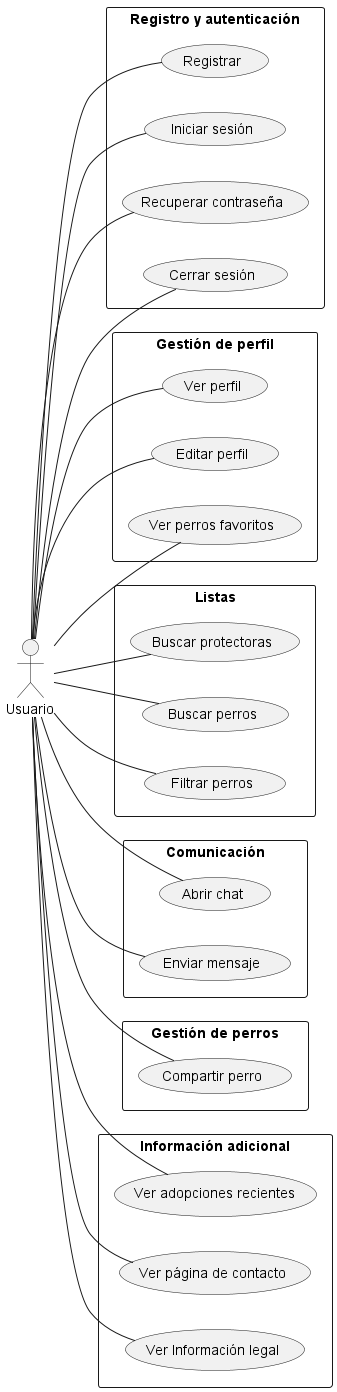
\includegraphics[width=5cm]{diagram/UserC.png}\par}
		\caption{Diagrama de casos de uso: usuario.}
	\end{center}
\end{figure}


%Caso de uso: Protectora
\begin{figure}[H]
	\begin{center}
		{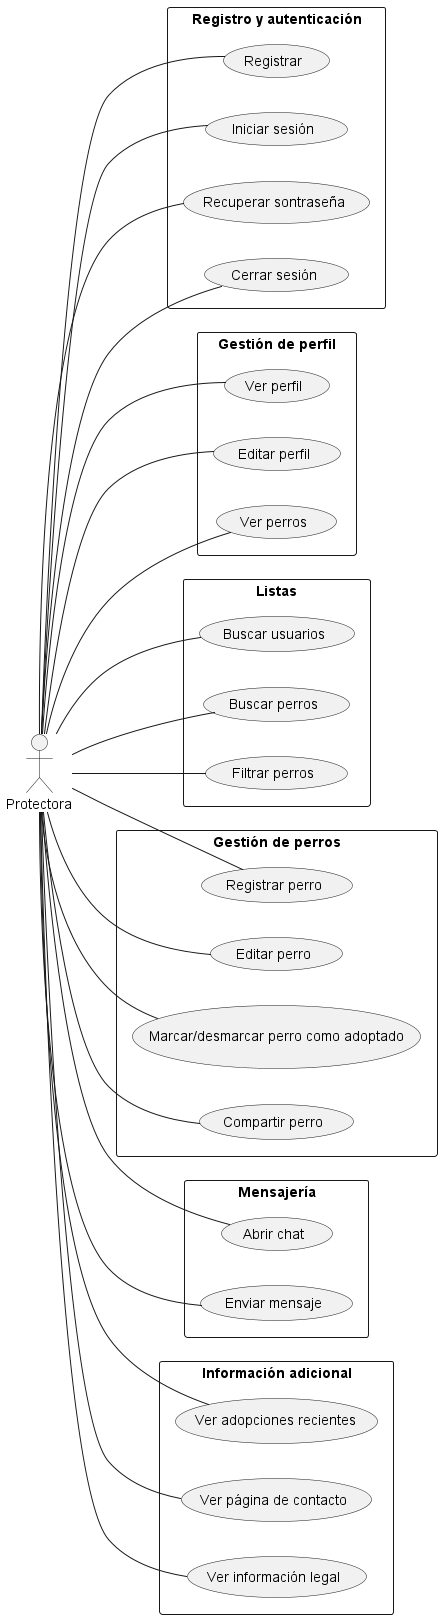
\includegraphics[width=5cm]{diagram/Shelter.png}\par}
		\caption{Diagrama de casos de uso: protectora.}
	\end{center}
\end{figure}


%Caso de uso: Administrador
\begin{figure}[H]
	\begin{center}
		{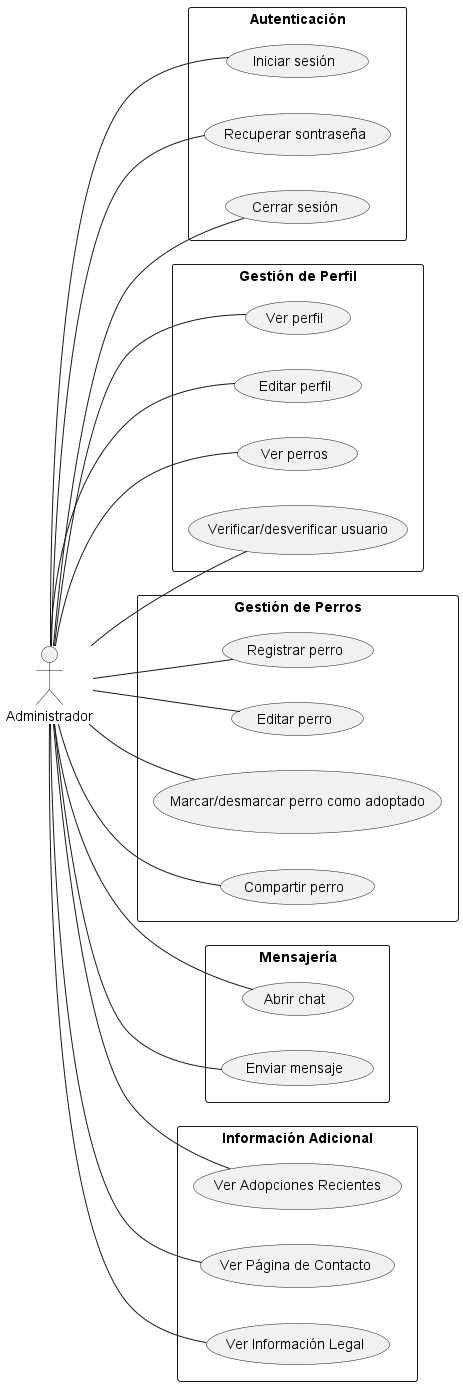
\includegraphics[width=5cm]{diagram/Admin.png}\par}
		\caption{Diagrama de casos de uso: administrador.}
	\end{center}
\end{figure}





% Recursos
\newpage
\section{Herramientas y software utilizado}

En esta sección se definen las herramientas y librerías necesarias para el desarrollo de la aplicación.

El sistema operativo utilizado es el que estaba instalado previamente en el ordenador personal, concretamente \textit{Windows 10}.

Para realizar el desarrollo, se ha utilizado \textit{Android Studio Hedgehog}. 


A la hora de seleccionar el framework para utilizar durante el desarrollo, se parte de que se necesita crear una aplicación Android. Existen diferentes frameworks disponibles, como \textit{React Native}, \textit{Flutter}, \textit{Kotlin Multiplatform}, etc., que ofrecen integración con Android para facilitar el desarrollo. En este proyecto, se ha optado por utilizar Flutter, dado que se ha trabajado previamente con él. Este framework, además, permite realizar un desarrollo multiplataforma y ofrece un alto rendimiento.

El lenguaje utilizado ha sido \textit{Dart}. Este lenguaje es muy similar a Java y está orientado a objetos. Se utiliza principalmente para el desarrollo de aplicaciones del lado del cliente. Es un lenguaje bastante popularizado. Uno de los motivos para optar por este lenguaje ha sido din duda el mantenimiento que recibe a día de hoy y su simplicidad para programar. Para añadir funcionalidades extra, se han escogido varias bibliotecas que ofrecen microservicios o widgets.

Por último, para la base de datos, se ha optado por utilizar \textit{Firebase}. Se trata de una plataforma de desarrollo de aplicaciones web muy popularizada, también desarrollada por Google. Ofrece diversos servicios para la autenticación, el \textit{hosting} de la aplicación y bases de datos en tiempo real. Esto lo convierte en el candidato adecuado para manejar funciones como el chat, la funcionalidad de compartir y otras características que la aplicación requiere.

\begin{itemize}[noitemsep]
	\item \textbf{Sistema Operativo:} Windows 11 x64
	\item \textbf{IDE:} Android Studio Hedgehog | 2023.1.1 Patch 2
	\item \textbf{Framework:} Flutter 3.19.0 -  Flutter DEV \cite{flutter_dev}
	\item \textbf{Lenguaje:} Dart 3.3.0 - Dart DEV \cite{dart_dev}
	\item \textbf{Paquetes:}
		\begin{itemize}[noitemsep]
		  \item \texttt{cupertino\_icons: \^{}1.0.2}
		  \item \texttt{firebase\_core: \^{}2.24.2}
		  \item \texttt{firebase\_database: \^{}10.3.8}
		  \item \texttt{firebase\_storage:}
		  \item \texttt{cloud\_firestore: \^{}4.13.6}
		  \item \texttt{firebase\_auth: \^{}4.15.3}
		  \item \texttt{responsive\_sizer: \^{}3.3.0+1}
		  \item \texttt{flutter\_login: \^{}5.0.0}
		  \item \texttt{google\_fonts: \^{}4.0.4}
		  \item \texttt{resize: \^{}1.0.0}
		  \item \texttt{awesome\_notifications: \^{}0.9.2}
		  \item \texttt{csc\_picker: \^{}0.2.7}
		  \item \texttt{map\_address\_picker: \^{}0.3.5}
		  \item \texttt{geocoding: \^{}3.0.0}
		  \item \texttt{search\_map\_location: 0.0.6}
		  \item \texttt{image\_picker: \^{}1.0.7}
		  \item \texttt{image\_cropper: \^{}4.0.1}
		  \item \texttt{path\_provider: \^{}2.1.2}
		  \item \texttt{flutter\_image\_compress: \^{}2.1.0}
		  \item \texttt{address\_form: \^{}0.0.2}
		  \item \texttt{address: \^{}0.1.0+2}
		  \item \texttt{google\_maps\_webservice: \^{}0.0.20-nullsafety.5}
		  \item \texttt{meta\_validator: \^{}0.0.2}
		  \item \texttt{geolocator: \^{}9.0.2}
		  \item \texttt{dropdown\_search: \^{}5.0.6}
		  \item \texttt{card\_swiper: \^{}3.0.1}
		  \item \texttt{filter\_list: \^{}1.0.2}
		  \item \texttt{flutter\_filter\_dialog: \^{}1.2.0}
		  \item \texttt{choice: \^{}2.3.2}
		  \item \texttt{animate\_gradient: \^{}0.0.2+1}
		  \item \texttt{firebase\_messaging: \^{}14.9.1}
		  \item \texttt{flutter\_chat\_bubble: \^{}2.0.2}
		  \item \texttt{chat\_bubbles: \^{}1.6.0}
		  \item \texttt{share\_plus: \^{}9.0.0}
		  \item \texttt{app\_links: \^{}6.0.1}
		  \item \texttt{url\_launcher: \^{}6.2.6}
		  \item \texttt{firebase\_dynamic\_links: \^{}5.5.4}
		  \item \texttt{go\_router: \^{}14.0.2}
		  \item \texttt{get: \^{}4.6.6}
		  \item \texttt{linkwell: \^{}2.0.6}
		  \item \texttt{toastification: \^{}1.0.0}
		\end{itemize}
	\item \textbf{Base de datos:} Firebase database - Firebase console \cite{firebase_console}
\end{itemize}

% Diseño
\newpage
\section{Diseño de la Aplicación}

En esta parte se incluye toda la estructura de la aplicación, es decir, tanto la interfaz de usuario como el backend y la base de datos.

\subsection{La base de datos}

Se deben almacenar todas las entidades y sus atributos, definiendo claramente el tipo de cada una.

\subsubsection{Guardado de usuarios}

Los usuarios son otra entidad de gran relevancia dentro de la aplicación. Aunque un usuario tiene bastantes datos dentro de la aplicación, muchos de ellos se almacenan en otras tablas y se accede a ellos referenciando sus IDs. Además, para manejar los registros de usuarios se utiliza el servicio de autenticación que proporciona Firebase, el cual facilita las herramientas para registrar usuarios y permite almacenar tanto el correo electrónico como la contraseña, entre otras cosas. En esta tabla se guarda toda la información de los usuarios, independientemente de su rol, que puede ser: \textbf{user}, \textbf{company} o \textbf{admin}, indicando si el usuario es un usuario estándar, una protectora o un administrador, respectivamente.

% usuarios
\begin{table}[H]
\captionsetup{justification=raggedright,singlelinecheck=false}
\captionsetup{labelformat=empty}
\caption{\textbf{Tabla: usuarios}}
\label{tab:requests}
	\begin{tabular}{|m{3.2cm}|m{2cm}|m{5cm}|m{3cm}|}
	\hline
	\textbf{Campo} & \textbf{Tipo} & \textbf{Dato} & \textbf{Obligatorio} \\ 
	\hline
	\textbf{chats} & array & IDs de los chats que pertenecen al usuario &  Sí \\ 
	\hline
	\textbf{email} & string &  ID del chat desde el que se manda la notificación &  Sí \\ 
	\hline
	\textbf{profilePic} & string & URL de la imagen de foto de perfil & Sí \\ 
	\hline
	\textbf{rol} & string & Rol del usuario & Sí \\ 
	\hline
	\textbf{username} & string & Nombre de usuario & Sí \\ 
	\hline
	\textbf{verified} & string & Indica si ha sido verificado por un administrador & Sí, solo si su rol es protectora \\ 
	\hline
	\end{tabular}
\end{table}



A continuación, se muestra un ejemplo de usuario guardado en la base de datos:

\begin{verbatim}
{
  "chats": [
    "wfmRPtHiGvUI9vi9Fs7k"
  ],
  "email": "protectora@test.com",
  "profilePic": "",
  "rol": "company",
  "username": "Protectora super chula",
  "verified": true
}
\end{verbatim}

\subsubsection{Guardado de caninos}

Esta entidad es una de las más importantes de la aplicación, ya que es la principal afectada por la mayoría de funcionalidades que se proponen. Principalmente, esta tabla contendrá todas las propiedades de los caninos que se manejarán dentro de la app, aunque hay algunas consideraciones importantes para algunas de ellas. Por ejemplo, para el género se han propuesto dos valores fijos que luego se transformarán en la cadena correspondiente cuando se carguen en la interfaz de usuario. Los valores son \textbf{male} y \textbf{female}. Se propone esta solución para cuando se decida a futuro añadir traducciones en la aplicación. Por otro lado, para almacenar la edad, se ha optado por hacerlo junto a las unidades, ya que así se le da al usuario la posibilidad de especificar mejor la edad del can (el caso de uso es muy concreto, pero añade valor). Los valores de las unidades son fijos, pudiendo ser:

\begin{itemize}[noitemsep]
	\item \textbf{Meses}
	\item \textbf{Años}
\end{itemize}

Lo mismo ocurre con el peso se opta por almacenarlo junto a las unidades. Independientemente de las unidades que marque el usuario, el peso en la base de datos siempre será tratado como Kg para facilitar el filtrado. Cuando se cargue en la interfaz de usuario, se mostrarán las unidades y el valor original, que pueden ser:

\begin{itemize}[noitemsep]
	\item \textbf{Gramos}
	\item \textbf{Kg}
\end{itemize}

Una alternativa sería almacenar los caninos favoritos en la tabla de usuarios. Sin embargo, almacenar los usuarios que han marcado al canino como favorito en esta tabla facilita las actualizaciones en tiempo real de los resultados. Se realizaron algunas pruebas con la primera alternativa que requería que para mostrar el número de veces que un canino estaba marcado como favorito, hubiera que consultar todas las entradas existentes de usuarios. Por otra parte, requería recargar constantemente los resultados de los caninos en las listas tras marcar o desmarcar un favorito, lo que reducía considerablemente el rendimiento de la aplicación. Con este modelo, se puede trabajar únicamente escuchando los cambios en las diferentes entradas de la tabla para los caninos y actualizar la información en pantalla en tiempo real sin comprometer el rendimiento. 

\begin{table}[H]
\captionsetup{justification=raggedright,singlelinecheck=false}
\captionsetup{labelformat=empty}
\caption{\textbf{Tabla: caninos}}
\label{tab:dogs}
	\begin{tabular}{|m{3cm}|m{2cm}|m{5cm}|m{3cm}|}
	\hline
	\textbf{Campo} & \textbf{Tipo} & \textbf{Dato} & \textbf{Obligatorio} \\ 
	\hline
	\textbf{adopted} & booleano & Indica si el can ha sido adoptado & Sí \\ 
	\hline
	\textbf{age} & número & Edad &  Sí \\ 
	\hline
	\textbf{ageUds} & string & Unidades de la edad & Sí \\ 
	\hline
	\textbf{breed} & string & Raza &  Sí \\ 
	\hline
	\textbf{castrated} & booleano & Indica si está castrado & Sí \\ 
	\hline
	\textbf{color} & string & Color & Sí \\ 
	\hline
	\textbf{created} & marca de tiempo & Fecha y hora de cuándo se ha dado de alta &  Sí \\ 
	\hline
	\textbf{description} & string & Descripción & No \\ 
	\hline
	\textbf{favoriteBy} & array & IDs de usuarios que lo han marcado como favorito & No \\ 
	\hline
	\textbf{forAdoption} & booleano & Indica si está disponible para adopción & No \\ 
	\hline
	\textbf{forFoster} & booleano & Indica si está disponible para acogida & No \\ 
	\hline
	\textbf{gender} & string & Género & Sí \\ 
	\hline
	\textbf{name} & string & Nombre & Sí \\ 
	\hline
	\textbf{ownerId} & string & ID del propietario &  Sí \\ 
	\hline
	\textbf{profilePic} & string & URL de la imagen de perfil de la mascota & No \\ 
	\hline
	\textbf{weight} & decimal & Peso & Sí \\ 
	\hline
	\textbf{weightUds} & string & Unidades de peso &  Sí \\ 
	\hline
\end{tabular}
\end{table}

A continuación, se muestra un ejemplo real de un canino almacenado en la base de datos:

\begin{verbatim}
{
  "adopted": false,
  "age": 1,
  "ageUds": "Años",
  "breed": "Breed 2",
  "castrated": true,
  "color": "Color 1",
  "created": "23 de abril de 2024, 10:56:48 a.m. UTC+2",
  "description": "",
  "favoriteBy": [],
  "forAdoption": true,
  "forFoster": true,
  "gender": "female",
  "name": "Katrina",
  "ownerId": "S4wXwckahiSOLI0Q3exXDVRh2yl2",
  "profilePic": "",
  "weight": 1,
  "weightUds": "KG"
}
\end{verbatim}


\subsubsection{Guardado de direcciones}

Para todas las protectoras, es necesario almacenar la dirección en la que están ubicadas. Esta información es crucial para mostrar a los usuarios la ubicación de cada protectora y generar marcadores en el mapa correspondiente. Por un lado, se almacenarán todas las partes de la dirección, como la ciudad, la calle, el código postal, etc. Por otro lado, cuando un usuario introduzca su dirección, se generarán automáticamente las coordenadas de esa dirección para almacenarlas también, evitando tener que calcularlas cada vez que se carguen los mapas en la interfaz. Asimismo, cuando un usuario actualice su dirección, se actualizarán también sus coordenadas correspondientes en la base de datos.

Para todas las direcciónes se genera una entrada en el que su ID corresponde con el del usuario al que pertenece.

% Addresses
\begin{table}[H]
\captionsetup{justification=raggedright,singlelinecheck=false}
\captionsetup{labelformat=empty}
\caption{\textbf{Tabla: direcciones}}
\label{tab:Addresses}
	\begin{tabular}{|m{3cm}|m{2cm}|m{5cm}|m{3cm}|}
	\hline
	\textbf{Campo} & \textbf{Tipo} & \textbf{Dato} & \textbf{Obligatorio} \\ 
	\hline
	\textbf{city} & string & Ciudad & Sí \\ 
	\hline
	\textbf{country} & string & País (España siempre) & Sí \\ 
	\hline
	\textbf{province} &  string & Provincia & Sí \\ 
	\hline
	\textbf{street} &  string & Calle &  Sí \\ 
	\hline
	\textbf{street\_number} &  string & Número de la calle & No\\ 
	\hline
	\textbf{zipcode} & string & Código postal &  Sí \\ 
	\hline
	\textbf{lat} & decimal & Latitud & Sí \\ 
	\hline
	\textbf{lng} & decimal & Longitud &  Sí \\ 
	\hline
\end{tabular}
\end{table}

A continuación, se muestra un ejemplo real de una dirección almacenada en la base de datos:

\begin{verbatim}
{
  "city": "Murcia",
  "country": "España",
  "lat": 37.9879153,
  "lng": -1.1315578,
  "province": "Murcia",
  "street": "Calle Maestro Alonso",
  "street_number": "4",
  "zipcode": "30005"
}
\end{verbatim}

\subsubsection{Guardado de chats}

Para la tabla de chats, se ha decidido almacenar los IDs de los usuarios implicados. Además, se guarda un array de IDs que indica para quién está disponible el chat en ese momento. Al igual que en otras aplicaciones de mensajería, cuando se elimina un chat, éste simplemente desaparece para el usuario que lo borra, lo que modifica la propiedad de quién puede acceder al chat en ese momento. Sin embargo, los mensajes no se borran. Por ejemplo, si una persona A borra su chat con la persona B y luego vuelve a abrir un chat con esa misma persona, los mensajes anteriores seguirán estando disponibles. Almacenar aquí los IDs de los usuarios implicados permite que, si se proponen chats de grupo, sea más sencillo escalarlo, ya que la base de datos ya lo está soportando. Lo mismo ocurre con la propiedad que hace referencia a qué usuarios pueden ver el chat. Para todos los chats se genera un ID automático, al que se hace referencia desde la tabla de usuarios.

% Chats
\begin{table}[H]
\captionsetup{justification=raggedright,singlelinecheck=false}
\captionsetup{labelformat=empty}
\caption{\textbf{Tabla: chats}}
\label{tab:chats}
	\begin{tabular}{|m{3cm}|m{2cm}|m{5cm}|m{3cm}|}
	\hline
	\textbf{Campo} & \textbf{Tipo} & \textbf{Dato} & \textbf{Obligatorio} \\ 
	\hline
	\textbf{availableTo} & array & IDs de usuarios que tienen el chat visible en su página &  Sí \\ 
	\hline
	\textbf{lastMessage} & string & ID del último mensaje mandado en el chat &  Sí \\ 
	\hline
	\textbf{users} &  array & IDs de usuarios que intervienen en el chat &  Sí  \\ 
	\hline
\end{tabular}
\end{table}

A continuación se muestra un ejemplo real de un chat almacenado en la base de datos: 

\begin{verbatim}
{
  "availableTo": [
    "kuaKjc6XoiVot1rMeGqBySA5pE13",
    "buO4Vkazs3O2oVKetugxrvTfRw12"
  ],
  "lastMessage": "BaKmuuo8debUTdSNsvw0",
  "users": [
    "kuaKjc6XoiVot1rMeGqBySA5pE13",
    "buO4Vkazs3O2oVKetugxrvTfRw12"
  ]
}
\end{verbatim}

\subsubsection{Guardado de mensajes}

Aparte de almacenar toda la información de los chats, es necesario almacenar los mensajes que se envían a través de los mismos. Además de guardar el contenido del mensaje, se propone hacer una diferenciación por tipos. Concretamente, dos: \textbf{default} e \textbf{image}, que indican si un mensaje es texto o imagen, respectivamente. Esta definición de tipos ayudará a determinar cómo cargar el contenido en la interfaz. Para todos los mensajes, se genera un ID automático que se puede referenciar desde la tabla de chats.

% Mensajes
\begin{table}[H]
\captionsetup{justification=raggedright,singlelinecheck=false}
\captionsetup{labelformat=empty}
\caption{\textbf{Tabla: mensajes}}
\label{tab:messages}
	\begin{tabular}{|m{3.2cm}|m{2cm}|m{5cm}|m{3cm}|}
	\hline
	\textbf{Campo} & \textbf{Tipo} & \textbf{Dato} & \textbf{Obligatorio} \\ 
	\hline
	\textbf{chatId} & string & ID del chat &  Sí \\ 
	\hline
	\textbf{from} & string & ID del emisor del mensaje &  Sí \\ 
	\hline
	\textbf{messageContent} & cadena & Contenido del mensaje &  Sí \\ 
	\hline
	\textbf{read} & booleano & Indica si el recpetor a leído el mensaje &  Sí \\ 
	\hline
	\textbf{sent} & marca de tiempo & Fecha y hora en la que se mandó el mensaje & Sí \\ 
	\hline
	\textbf{to} & string & ID del receptor del mensaje & Sí \\ 
	\hline
	\textbf{type} & string & Tipo del mensaje & Sí \\ 
	\hline
	\end{tabular}
\end{table}

A continuación, se muestra un ejemplo real de un mensaje almacenado en la base de datos:

\begin{verbatim}
{
  "chatId": "Sm1Ji0chb9uhofa20VW5",
  "from": "kuaKjc6XoiVot1rMeGqBySA5pE13",
  "messageContent": "Hola, ¿estás?",
  "read": true,
  "sent": "6 de mayo de 2024, 1:57:30 a.m. UTC+2",
  "to": "buO4Vkazs3O2oVKetugxrvTfRw12",
  "type": "default"
}
\end{verbatim}


\subsubsection{Guardado de notificaciones}

En \textit{Firebase}, a las tablas se les llama colecciones y dentro de cualquier colección se pueden incluir subcolecciones. Usar subcolecciones evita la necesidad de referenciar los datos a través de IDs de entradas de otras tablas. En el caso de la tabla de notificaciones, se ha definido que para cada usuario se genera una entrada en la tabla, y dentro de cada entrada se crea una colección para las peticiones. Al iniciar sesión, se añade un \textit{listener} que escucha todos los cambios de esta tabla, y cuando llega una nueva solicitud, se envía una notificación a través del canal correspondiente. Cuando el usuario receptor recibe la notificación, esta solicitud se marca como vista. El ID de cada entrada en la tabla de notificaciones corresponde al ID del usuario al que pertenece.

% notifications
\begin{table}[H]
\captionsetup{justification=raggedright,singlelinecheck=false}
\captionsetup{labelformat=empty}
\caption{\textbf{Tabla: notificaciones}}
\label{tab:notifications}
	\begin{tabular}{|m{3.2cm}|m{2cm}|m{5cm}|m{3cm}|}
	\hline
	\textbf{Campo} & \textbf{Tipo} & \textbf{Dato} & \textbf{Obligatorio} \\ 
	\hline
	\textbf{requests} & collection & Colección de peticiones &  Sí \\ 
	\hline
	\end{tabular}
\end{table}

A continuación, se muestra la estructura de la colección de peticiones:

% requests
\begin{table}[H]
\captionsetup{justification=raggedright,singlelinecheck=false}
\captionsetup{labelformat=empty}
\caption{\textbf{Tabla: peticiones}}
\label{tab:users}
	\begin{tabular}{|m{3.2cm}|m{2cm}|m{5cm}|m{3cm}|}
	\hline
	\textbf{Campo} & \textbf{Tipo} & \textbf{Dato} & \textbf{Obligatorio} \\ 
	\hline
	\textbf{body} & string & Contenido de la notificación &  Sí \\ 
	\hline
	\textbf{chatId} & string &  ID del chat desde el que se manda la notificación &  Sí \\ 
	\hline
	\textbf{new} & booleano & Indica si la notificación se ha mostrado o no &  Sí \\ 
	\hline
	\textbf{summary} & string & Vista previa de la notificación &  Sí \\ 
	\hline
	\textbf{title} & string & Titulo de la notificacion &  Sí \\ 
	\hline
	\textbf{userId} & string & Usuario que manda la notifiación &  Sí \\ 
	\hline
	\end{tabular}
\end{table}

A continuación, se muestra una petición real almacenada en la base de datos:

\begin{verbatim}
{
  "body": "Hola, ¿cómo estás?",
  "chatId": "Sm1Ji0chb9uhofa20VW5",
  "new": false,
  "summary": "Hola, ¿cómo estás?",
  "title": "Laura Vega Palacios",
  "userId": "kuaKjc6XoiVot1rMeGqBySA5pE13"
}
\end{verbatim}

\subsubsection{Almacenamiento de imágenes}

En cuanto al almacenamiento de imágenes, se ha utilizado el servicio que proporciona Firebase llamado \textit{Storage}. Este servicio permite almacenar imágenes, vídeos y audios y viene integrado de manera nativa con otros de sus servicios, como el de \textit{Authentication} mencionado anteriormente. Dentro del almacenamiento reservado para la aplicación, se ha organizado según la siguiente jerarquía de directorios:

\begin{itemize}[noitemsep]
	\item \textit{images}
	\begin{itemize}[noitemsep]
		\item \textit{chats}
		\item \textit{profilePics}
	\end{itemize}
\end{itemize}

Las imágenes de perfil de usuarios y caninos se almacenan en el directorio \textit{profilePics}. Por otro lado, cuando se manda una imagen por chat, ésta se almacena en el directorio \textit{chats}. Para trabajar con las imágenes dentro de la aplicación, se pueden obtener los enlaces que se generan cuando se van almacenando dentro de \textit{Storage}. Estas URLs obtenidas se almacenan en las tablas definidas anteriormente. Si una de las imágenes es borrada, se tiene que borrar su referencia en la tabla de la base de datos y la imagen almacenada en \textit{Storage}.

\subsection{Prototipado de la interfaz de usuario}

El diseño de la Interfaz de Usuario (UI) se centra en crear una Experiencia de Usuario (UX) intuitiva y atractiva. Inicialmente, se define un estilo y tema que se debe mantener a lo largo de todos los bocetos o prototipos a generar. Es importante tener en cuenta que el diseño sea \textit{responsive} para que se adapte adecuadamente a todos los dispositivos móviles.

\subsubsection{Tema}

Para los colores principales de la aplicación, se ha optado por escoger el color morado, el cuál dentro de UX puede evocar diferentes sensaciones en el usuario. Muchas marcas de lujo utilizan este color para sus logos, aunque también puede evocar sentimientos de calma o relajación según las tonalidades que se utilicen. Teniendo el morado como color principal, se ha añdido a la paleta su color análogo: el azul. Para finalizar los colores principales, a la paleta se ha incluido el color complementario del azul, que es el naranja. Estos tres colores conforman los elementos de la aplicación: el morado se utiliza para la mayoría de los elementos, indicando que son importantes. El azul se mezcla con el morado en algunos elementos para hacer más dinámicos los fondos y utilizarlo en elementos no tan relevantes. Por último, el naranja es un color que se ha utilizado como acento o para llamar la atención del usuario. Junto a él se podrán utilizan algunos de sus colores análogos como el amarillo o el rojo. Finalmente, a la paleta de colores se ha añadido el color blanco roto pues es adecuado para los fondos de la aplicación.

\begin{figure}[H]
	\begin{center}
		{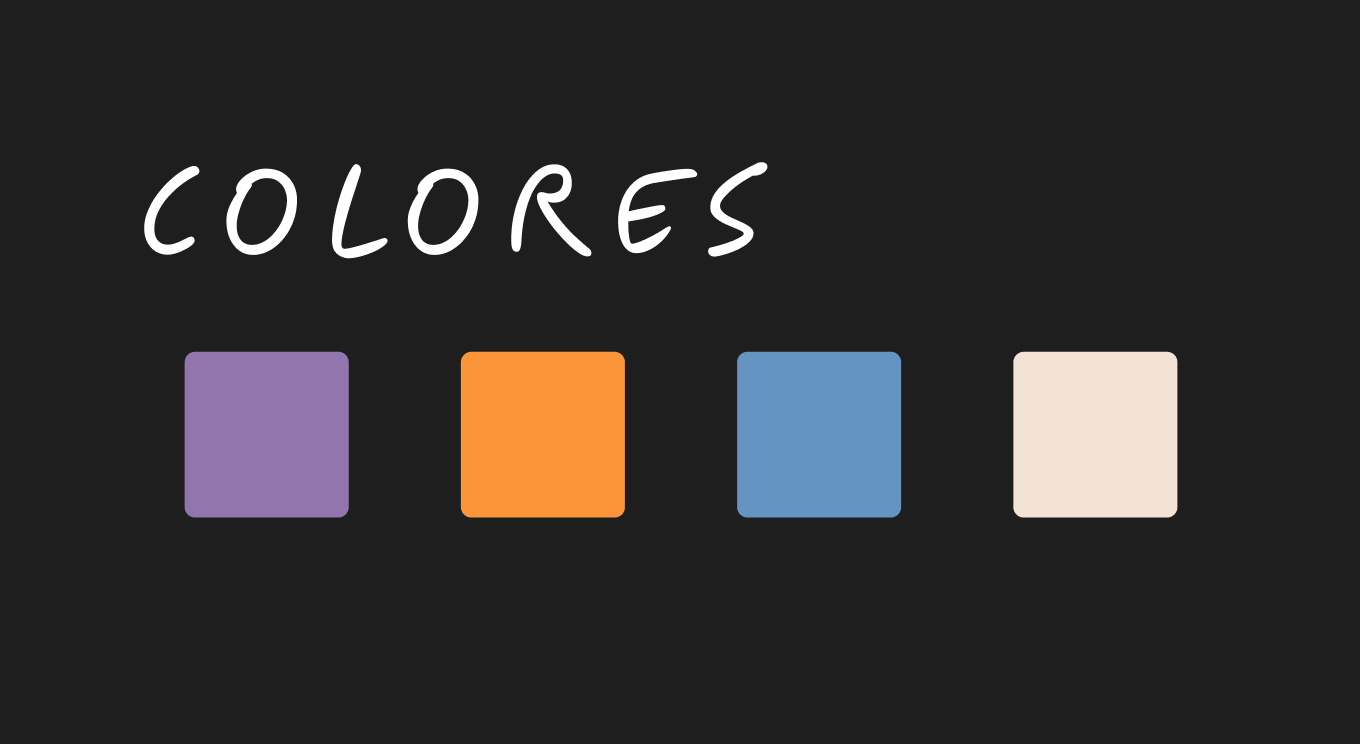
\includegraphics[width=7cm]{design/Colors.jpg}\par}
		\caption{Paleta de colores utilizada en la aplicación.}
	\end{center}
\end{figure}

Como fuente, se opta por escoger la \textit{Nunito Sans}, que proporciona Google. Su elección se debe a que es una fuente bastante estándar y legible para cualquier tipo de usuario.

\begin{figure}[H]
	\begin{center}
		{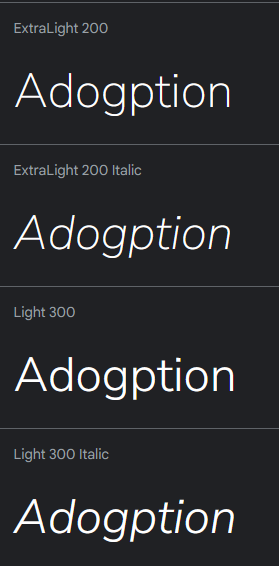
\includegraphics[width=7cm]{design/NunitoFont.png}\par}
		\caption{Fuente utilizada en la aplicación (\textit{Nunito Sans}).}
	\end{center}
\end{figure}

\subsubsection{Nombre}

Como nombre de la aplicación,  se ha tenido en cuenta que inicialmente la aplicación está dirigida a la adopción de caninos, así que se propone un juego de palabras. Uniendo las palabras \textit{Adoption} y \textit{Dog}, que son la traducción de las palabras adopción y perro, conformando el nombre: \textbf{\textit{Adogption}}.

\subsubsection{Logo e iconos}

La última parte relacionada con el \textit{branding} en este proyecto es la de generación de logos e iconos. En esta sección, se incluye tanto el logo de la aplicación como los iconos que conforman la misma. Algunos de los iconos podrían finalmente no utilizarse. La idea del logo es que se perciba claramente que la aplicación trata sobre ellos. Los \textit{Corgis} son una de las razas más populares en el mundo. Destacan por ser muy amigables y queridos dentro de la cultura \textit{pop}, lo que los convierte en la cara perfecta para llamar la atención. Además del logo principal, se ha diseñado uno animado para incluir en pantallas de carga u otros lugares. Por último, se han hecho algunos iconos por defecto que serán utilizados en perfiles o listas.


\begin{figure}[H]
   	\begin{subfigure}{0.48\textwidth}
		\begin{center}
			{
\includegraphics[width=3cm]{logo/Logo1.png}\par}
			\caption{Público.}
		\end{center}  
	\end{subfigure}\hfill
   	\begin{subfigure}{0.48\textwidth}
		\begin{center}
			{
\includegraphics[width=4cm]{logo/ADOGPTIONFIXED.png}\par}
			\caption{Animado.}
		\end{center}  
	\end{subfigure}\hfill
	\caption{Logos principales de la aplicación.}
\end{figure}

\begin{figure}[H]
   	\begin{subfigure}{0.48\textwidth}
		\begin{center}
			{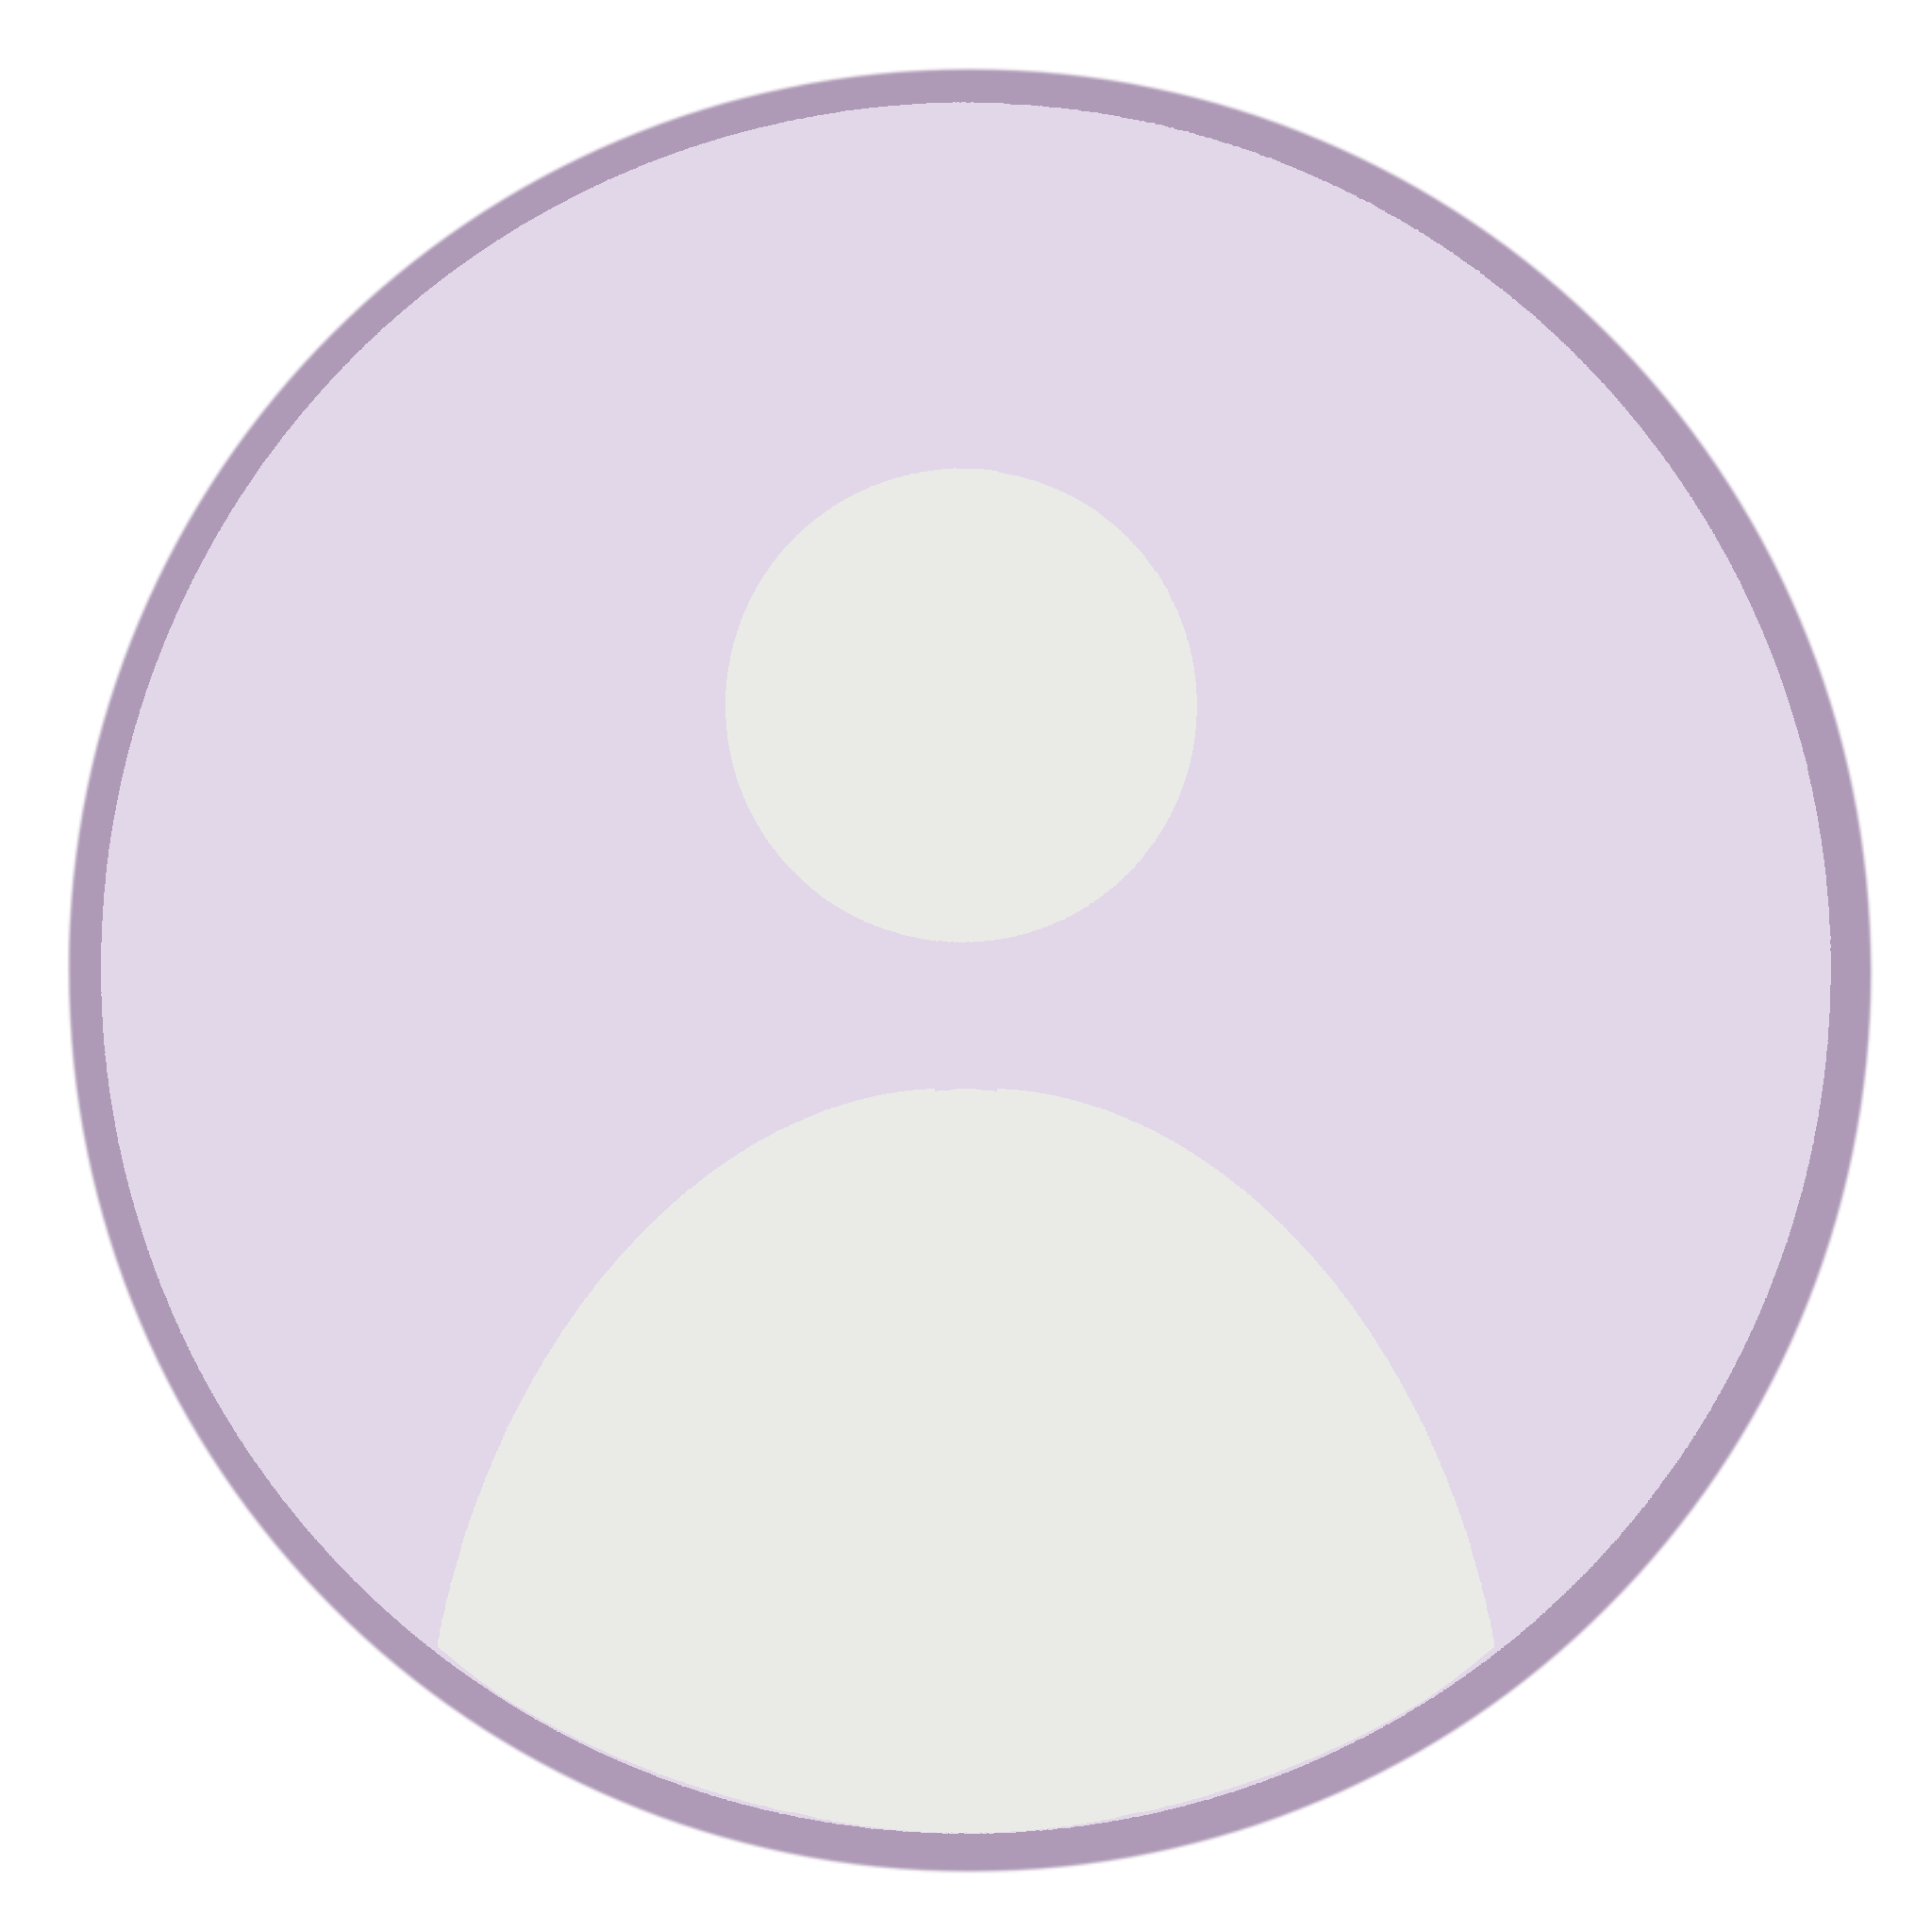
\includegraphics[width=3cm]{logo/EMPTYUSER.png}\par}
			\caption{Usuario.}
		\end{center}  
	\end{subfigure}\hfill
   	\begin{subfigure}{0.48\textwidth}
		\begin{center}
			{
\includegraphics[width=3cm]{logo/EMPTYDOG.png}\par}
			\caption{Canino.}
		\end{center}  
	\end{subfigure}\hfill
	\caption{Logo por defecto.}
\end{figure}


\begin{figure}[H]
   	\begin{minipage}{0.48\textwidth}
		\begin{center}
			{
\includegraphics[width=3cm]{logo/Adoptar.png}\par}
			\caption{Icono para listas de adopción.}
		\end{center}  
	\end{minipage}\hfill
   	\begin{minipage}{0.48\textwidth}
		\begin{center}
			{
\includegraphics[width=3cm]{logo/Acoger.png}\par}
			\caption{Icono para listas de acogida.}
		\end{center}  
	\end{minipage}\hfill
\end{figure}

\begin{figure}[H]
   	\begin{minipage}{0.48\textwidth}
		\begin{center}
			{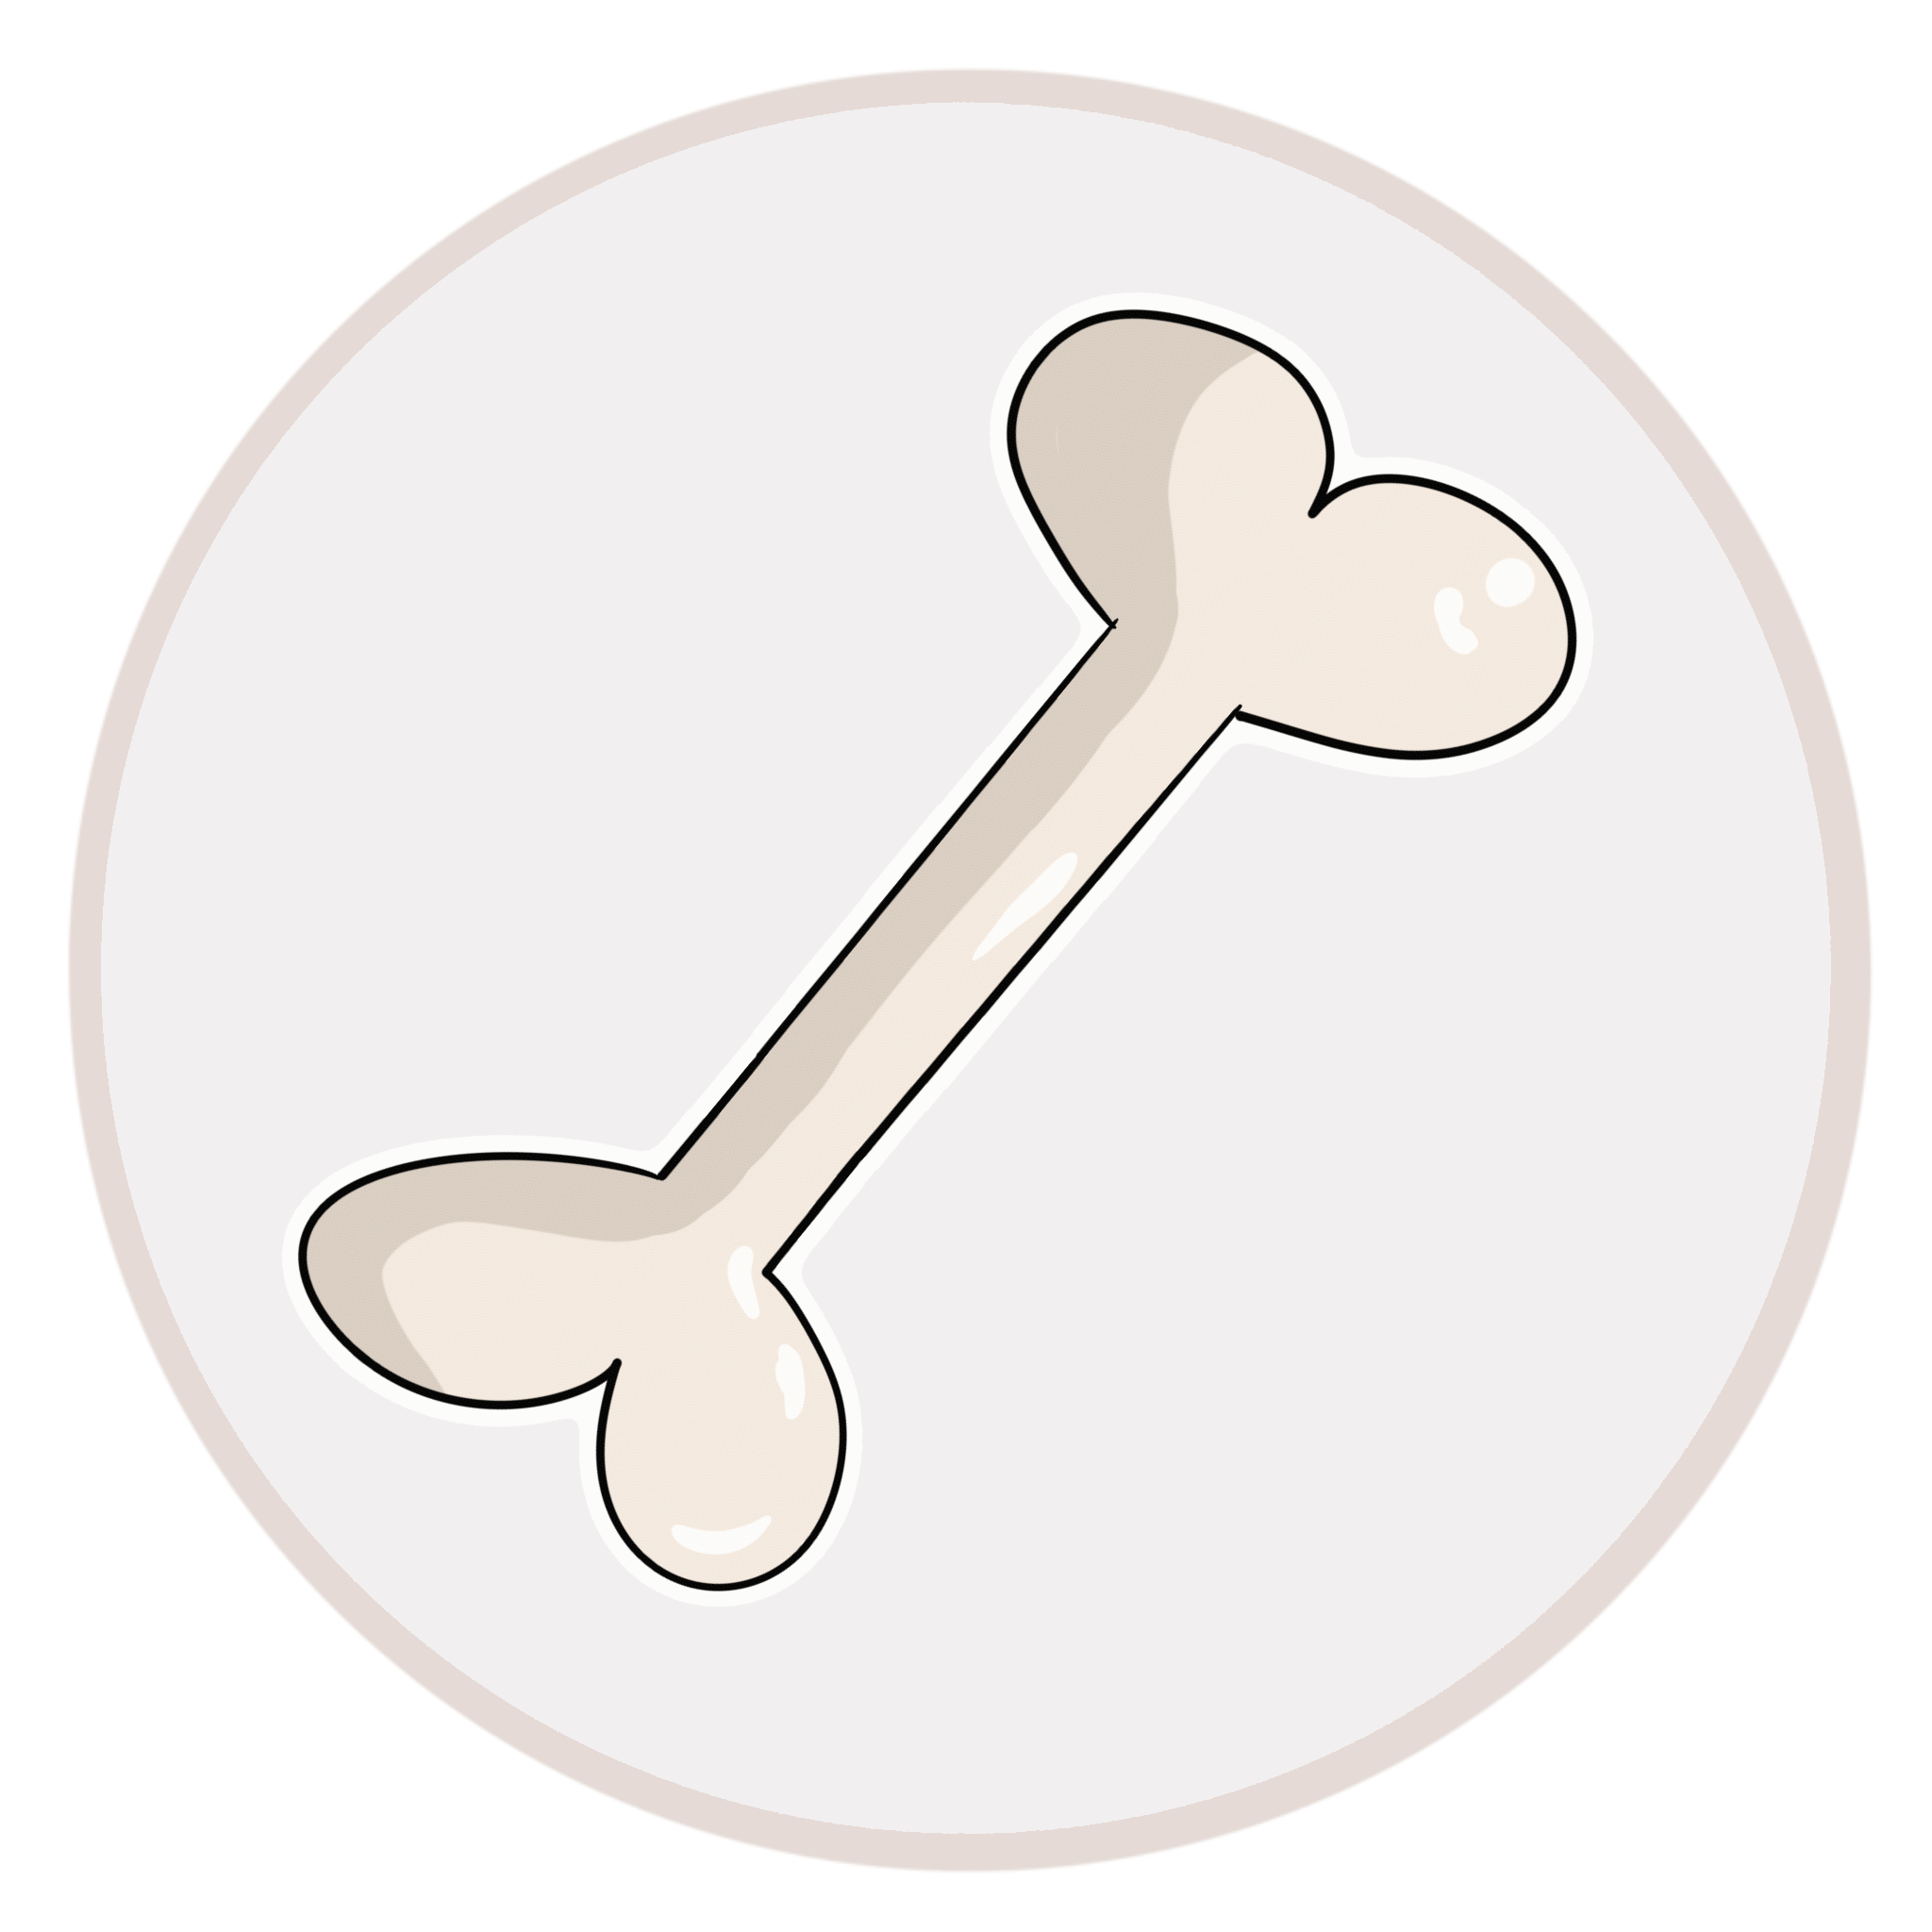
\includegraphics[width=3cm]{logo/Protectora.png}\par}
			\caption{Icono de hueso.}
		\end{center}  
	\end{minipage}\hfill
   	\begin{minipage}{0.48\textwidth}
		\begin{center}
			{
\includegraphics[width=3cm]{logo/Casa.png}\par}
			\caption{Icono de casa.}
		\end{center}  
	\end{minipage}\hfill
\end{figure}


\begin{figure}[H]
   	\begin{subfigure}{0.48\textwidth}
		\begin{center}
			{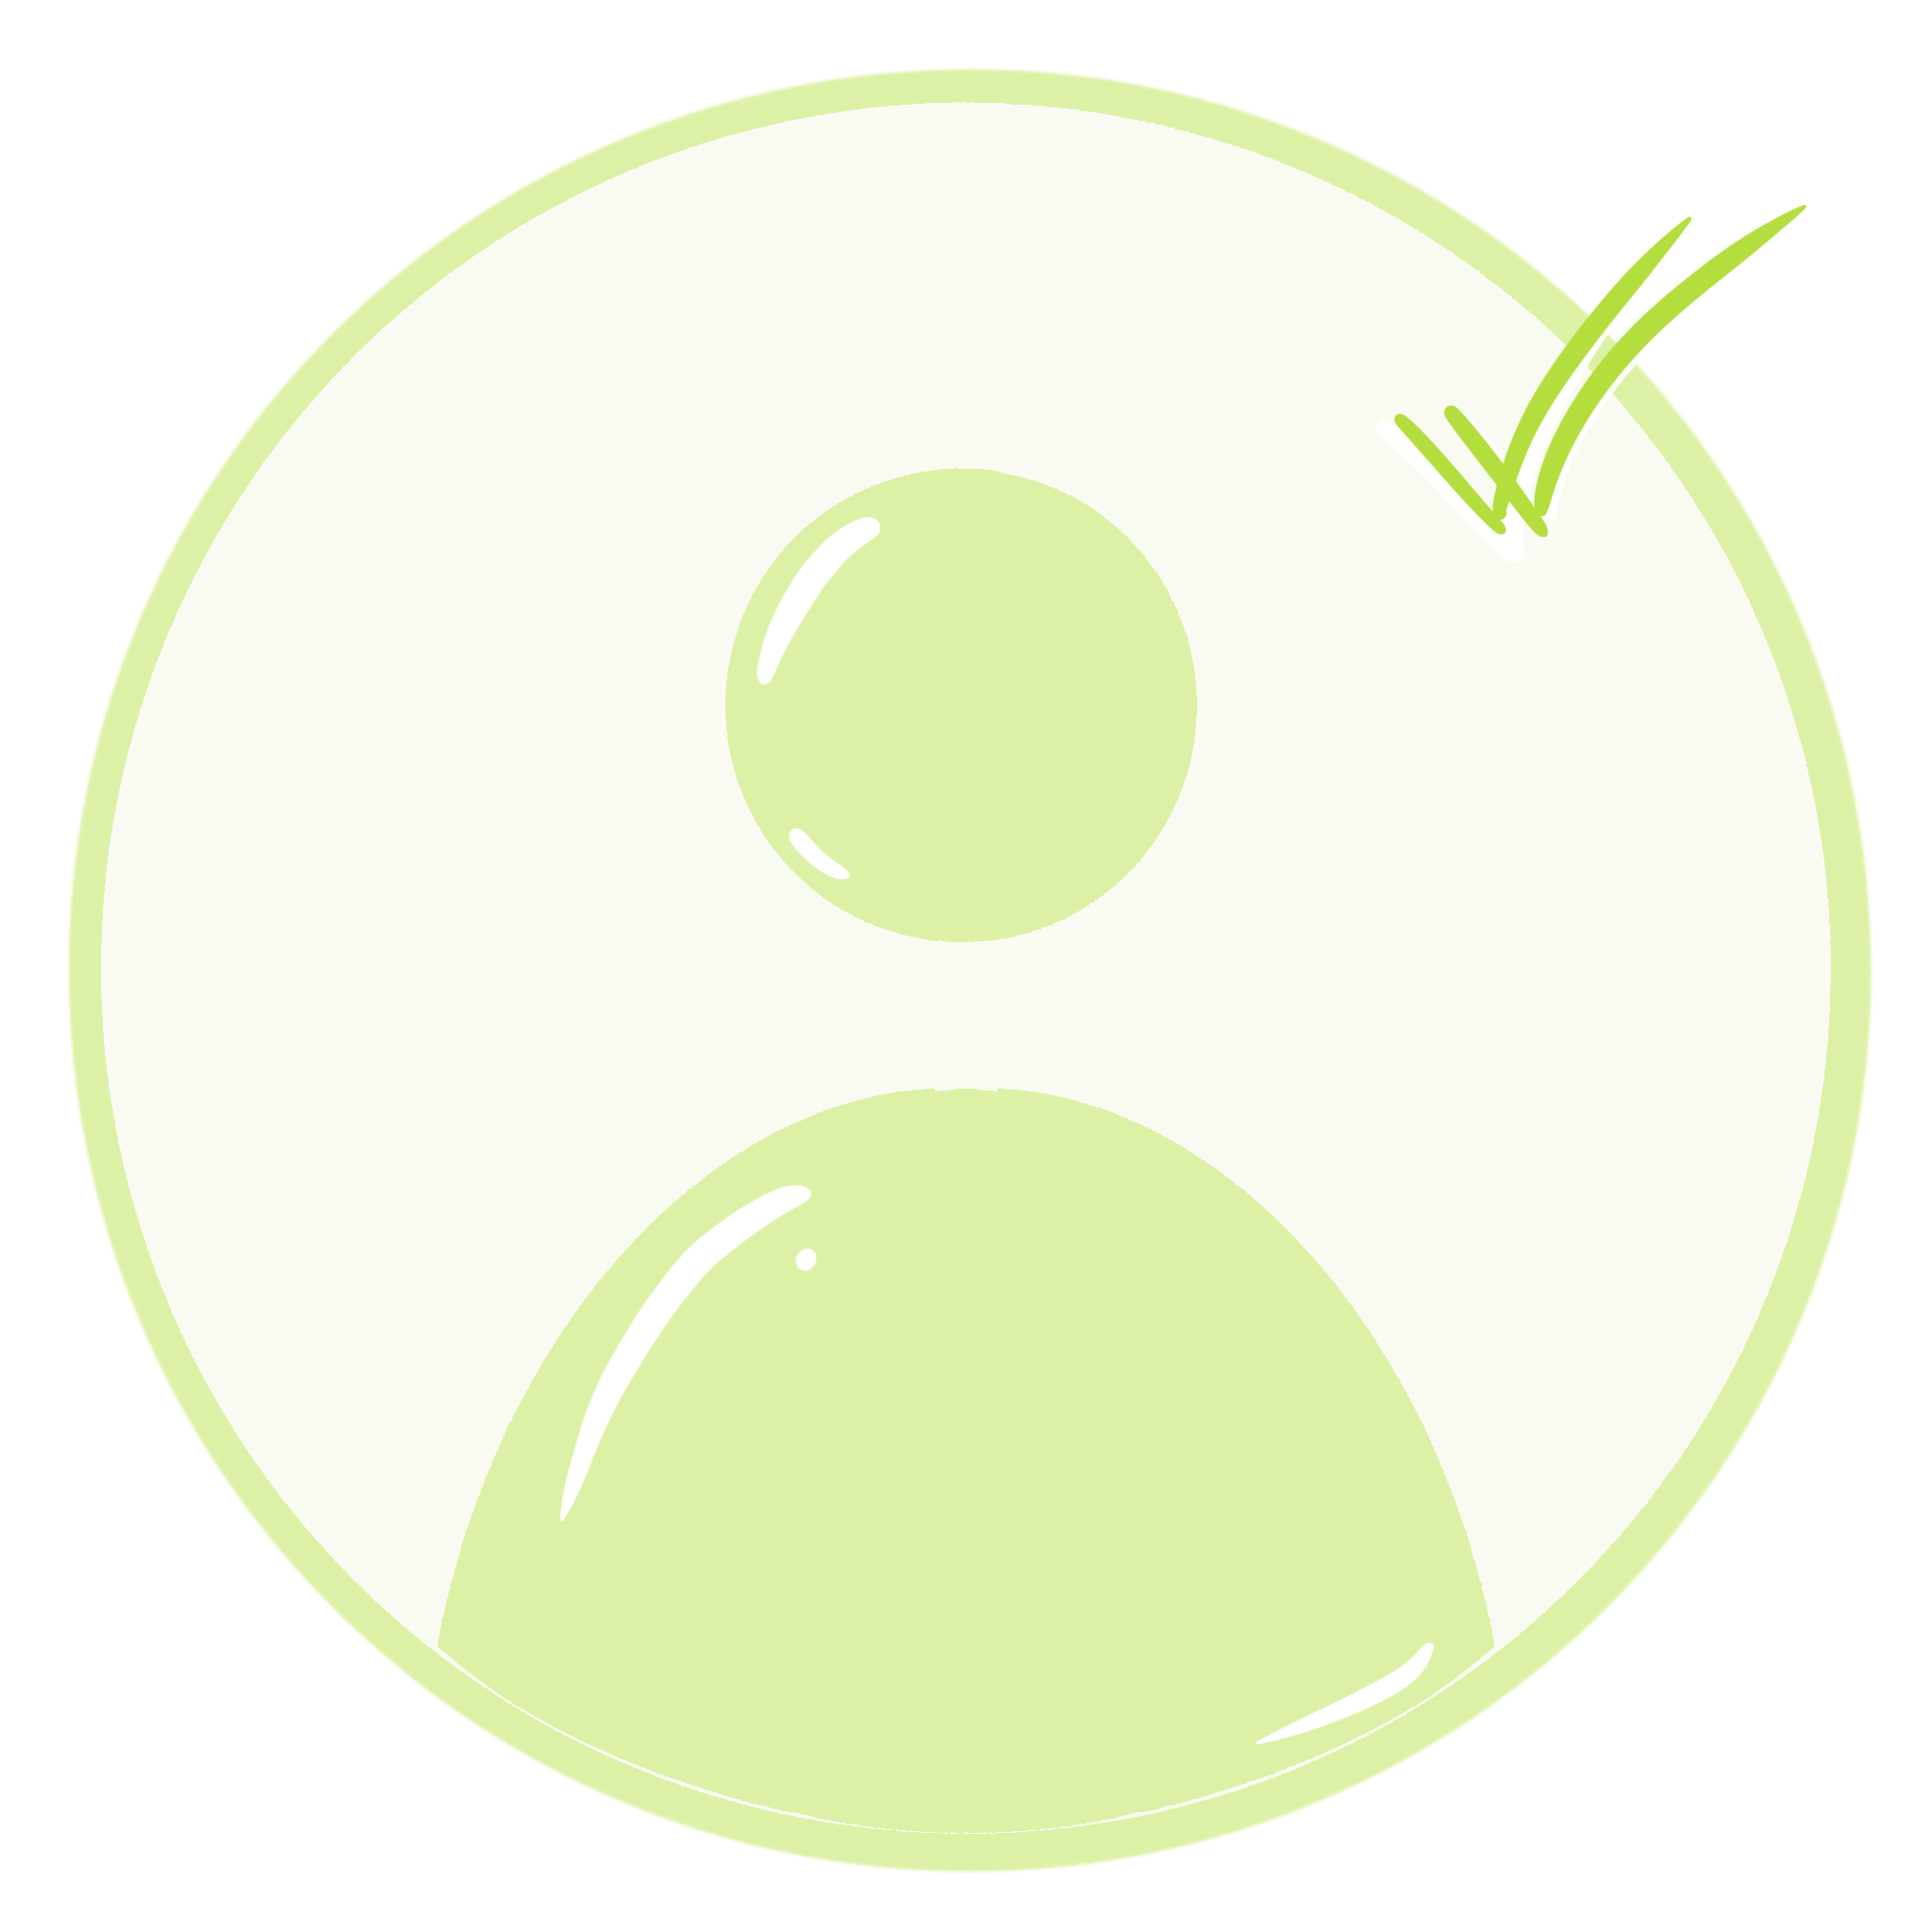
\includegraphics[width=3cm]{logo/USERV.png}\par}
			\caption{Verificado.}
		\end{center}  
	\end{subfigure}\hfill
   	\begin{subfigure}{0.48\textwidth}
		\begin{center}
			{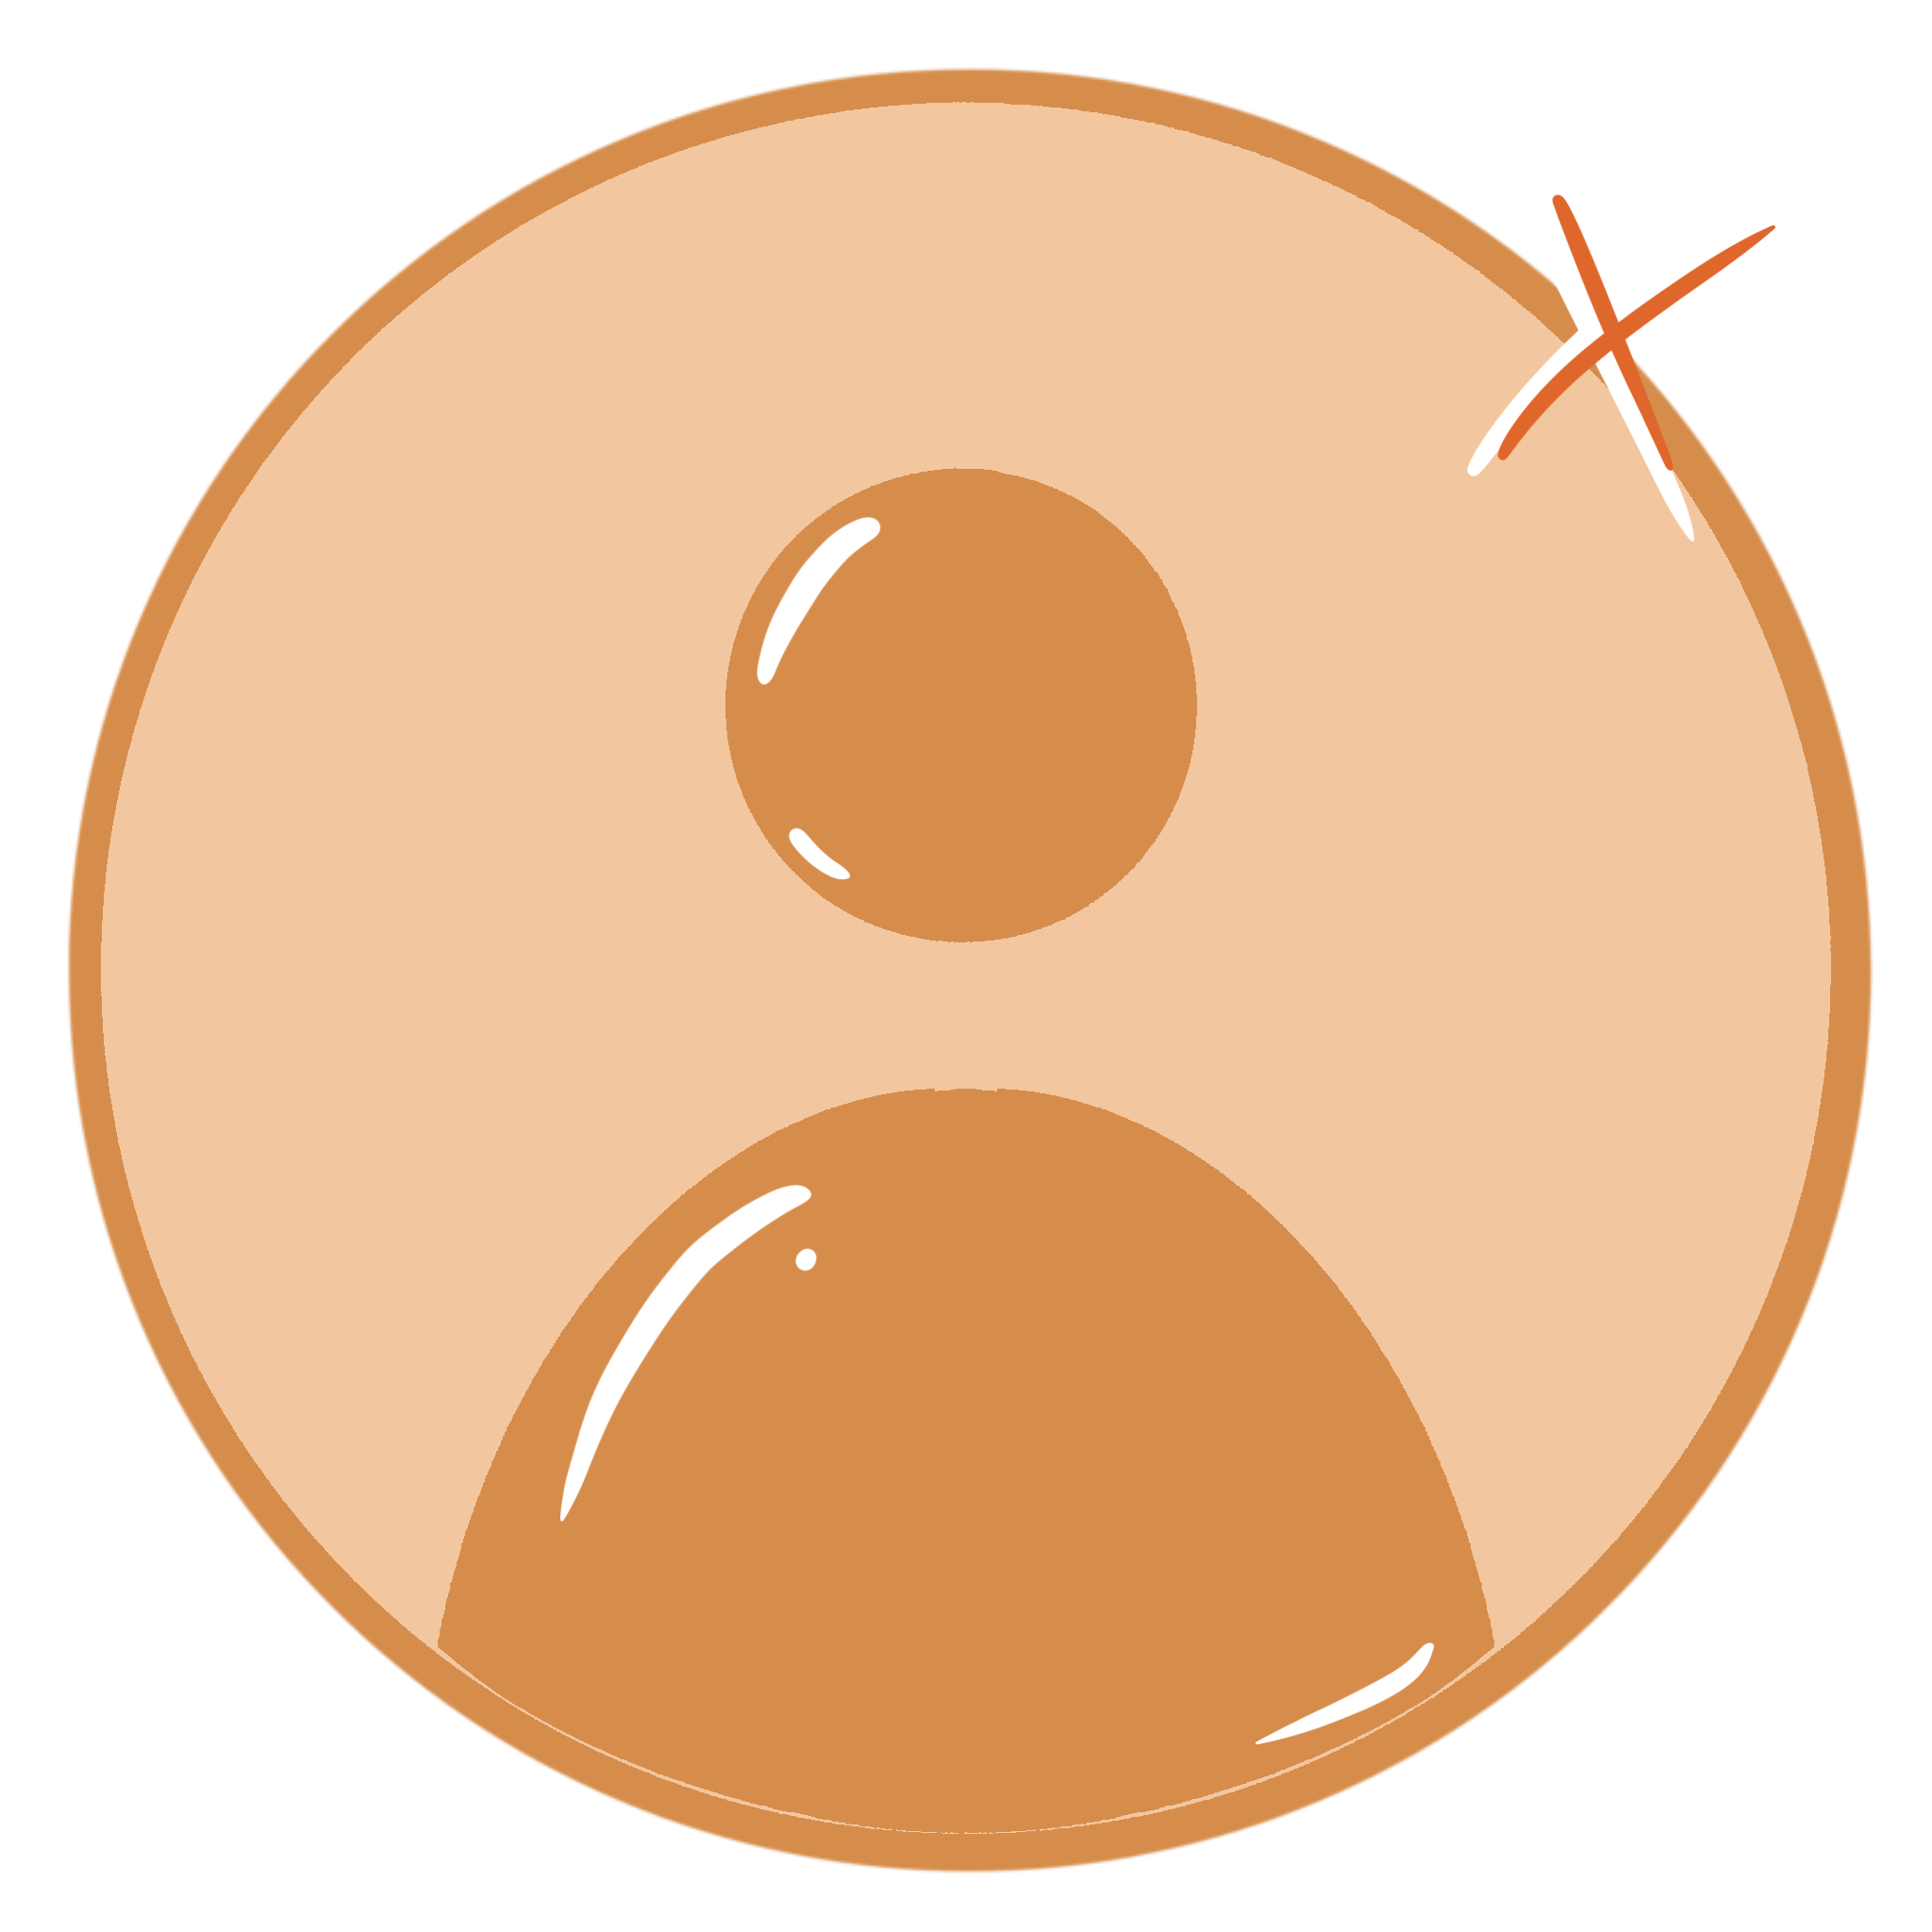
\includegraphics[width=3cm]{logo/USERNV.png}\par}
			\caption{No verificado.}
		\end{center}  
	\end{subfigure}\hfill
   	\begin{subfigure}{0.48\textwidth}
		\begin{center}
			{
\includegraphics[width=3cm]{logo/ALLUSER.png}\par}
			\caption{Color morado.}
		\end{center}  
	\end{subfigure}\hfill
   	\begin{subfigure}{0.48\textwidth}
		\begin{center}
			{
\includegraphics[width=3cm]{logo/USER.png}\par}
			\caption{Color azul.}
		\end{center}  
	\end{subfigure}\hfill
	\caption{Iconos usuarios.}
\end{figure}

\begin{figure}[H]
   	\begin{subfigure}{0.48\textwidth}
		\begin{center}
			{
\includegraphics[width=3cm]{logo/Pata1.png}\par}
			\caption{Color naranja.}
		\end{center}  
	\end{subfigure}\hfill
   	\begin{subfigure}{0.48\textwidth}
		\begin{center}
			{
\includegraphics[width=3cm]{logo/Pata2.png}\par}
			\caption{Color morado.}
		\end{center}  
	\end{subfigure}\hfill
   	\begin{subfigure}{0.48\textwidth}
		\begin{center}
			{
\includegraphics[width=3cm]{logo/Pata3.png}\par}
			\caption{Color morado.}
		\end{center}  
	\end{subfigure}\hfill
	\caption{Iconos de patas.}
\end{figure}


\newpage
\subsubsection{Diseños}

En esta sección, se incluyen todos los diseños realizados en \textit{Miro} para las pantallas principales de la aplicación y componentes relevantes. En la sección de implementación se especificará la función de cada una de las pantallas.


\begin{figure}[H]
   	\begin{minipage}{0.48\textwidth}
		\begin{center}
			{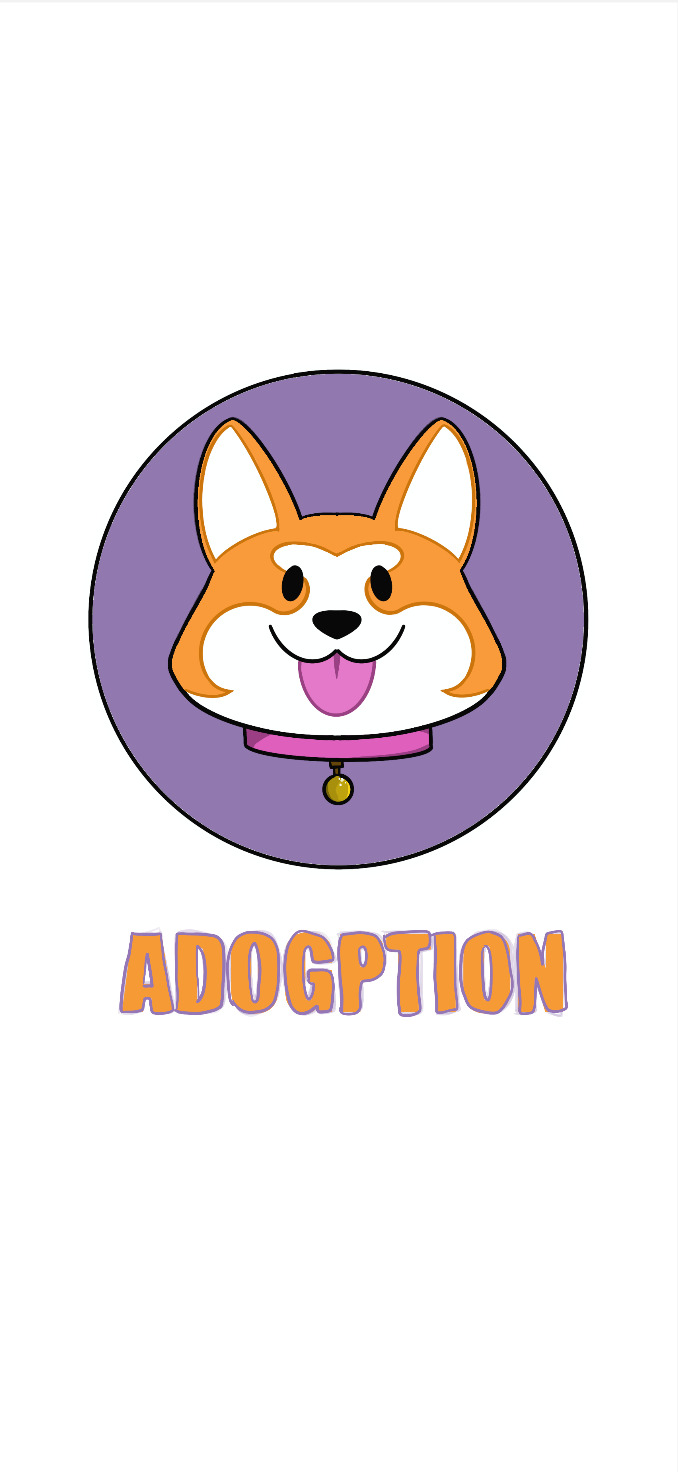
\includegraphics[height=8cm]{design/SplashScreen.jpg}\par}
			\caption{Pantalla de carga.}
			\medskip
		\end{center}  
	\end{minipage}\hfill
   	\begin{minipage}{0.48\textwidth}
		\begin{center}
			{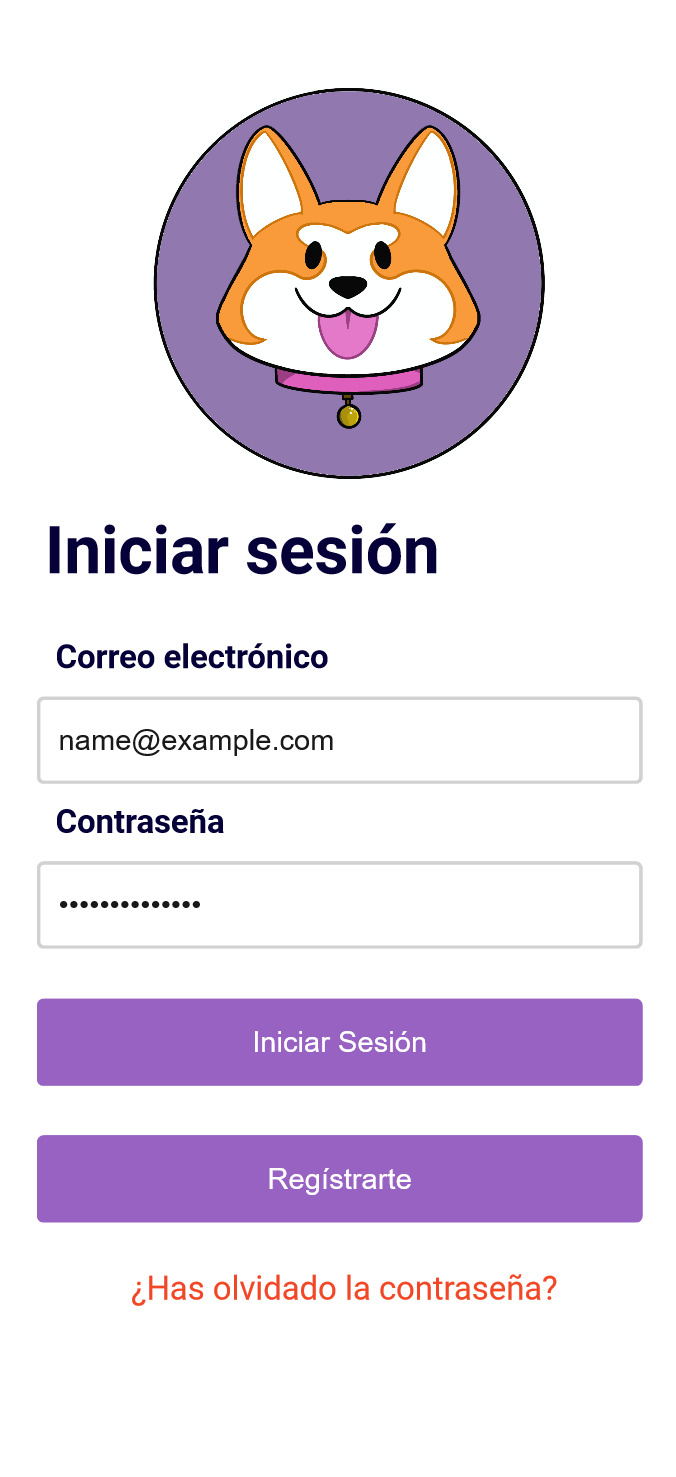
\includegraphics[height=8cm]{design/Login.jpg}\par}
			\caption{Pantalla de inicio de sesión.}
			\medskip
		\end{center}  
	\end{minipage}\hfill
\end{figure}


\begin{figure}[H]
   	\begin{minipage}{0.48\textwidth}
		\begin{center}
			{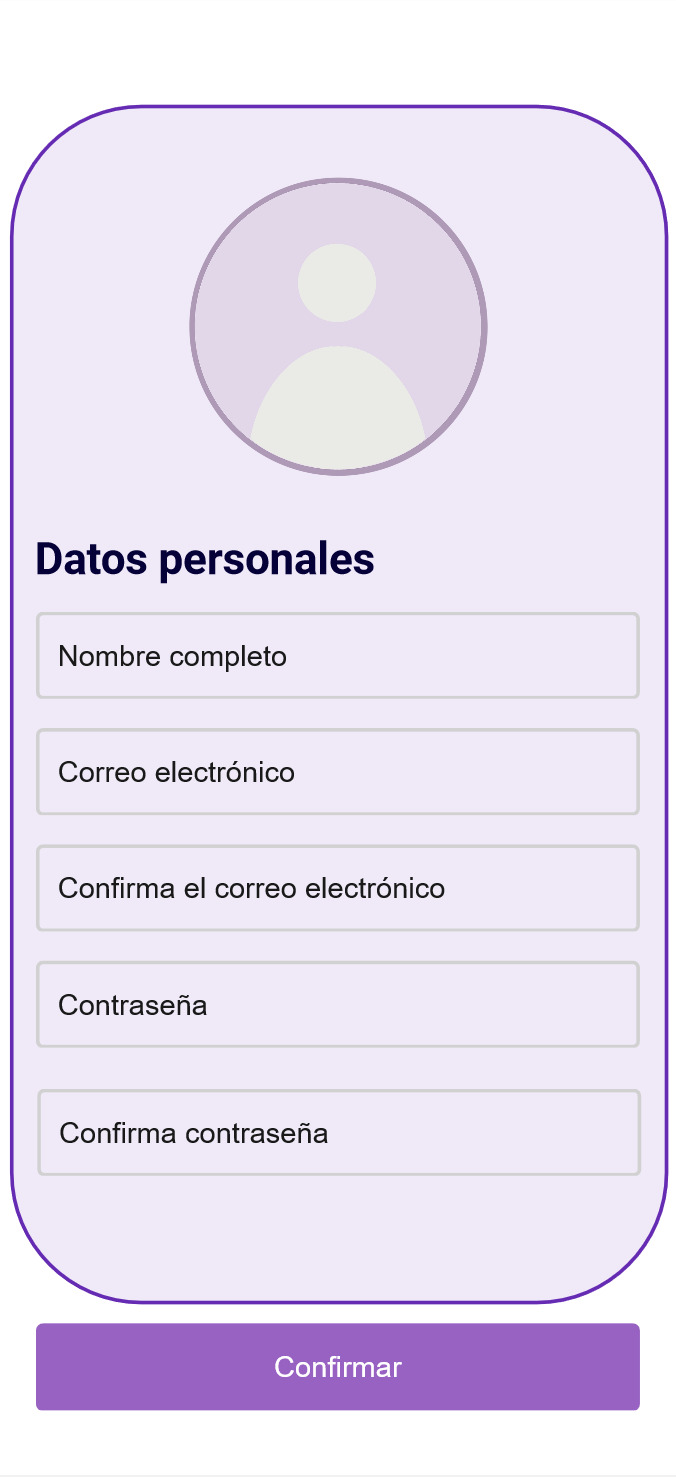
\includegraphics[height=8cm, width=4cm]{design/UserRegister.jpg}\par}
			\caption{Pantalla de registro/edición de usuario.}
			\medskip
		\end{center}  
	\end{minipage}\hfill
   	\begin{minipage}{0.48\textwidth}
		\begin{center}
			{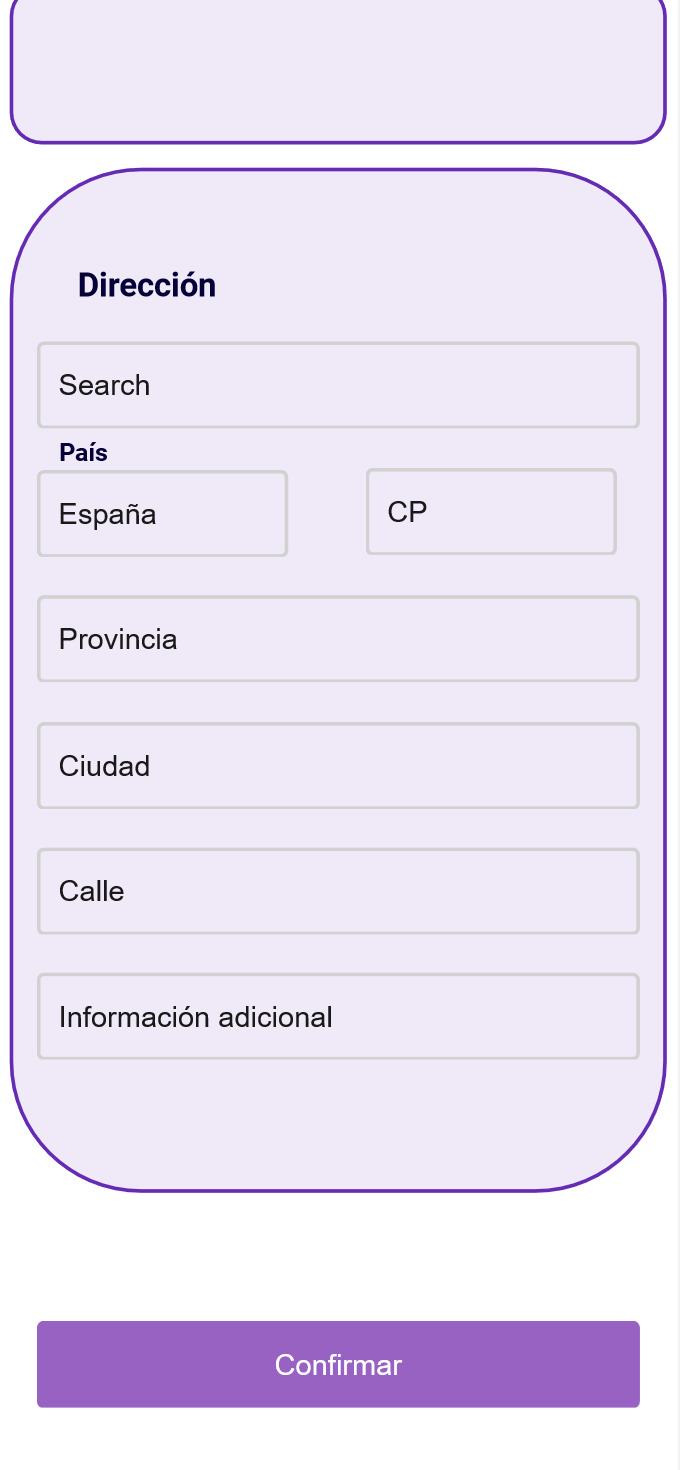
\includegraphics[height=8cm, width=4cm]{design/CompanyRegister.jpg}\par}
			\caption{Pantalla de registro/edición de protectora.}
			\medskip
		\end{center}  
	\end{minipage}\hfill
\end{figure}

\begin{figure}[H]
   	\begin{minipage}{0.48\textwidth}
		\begin{center}
			{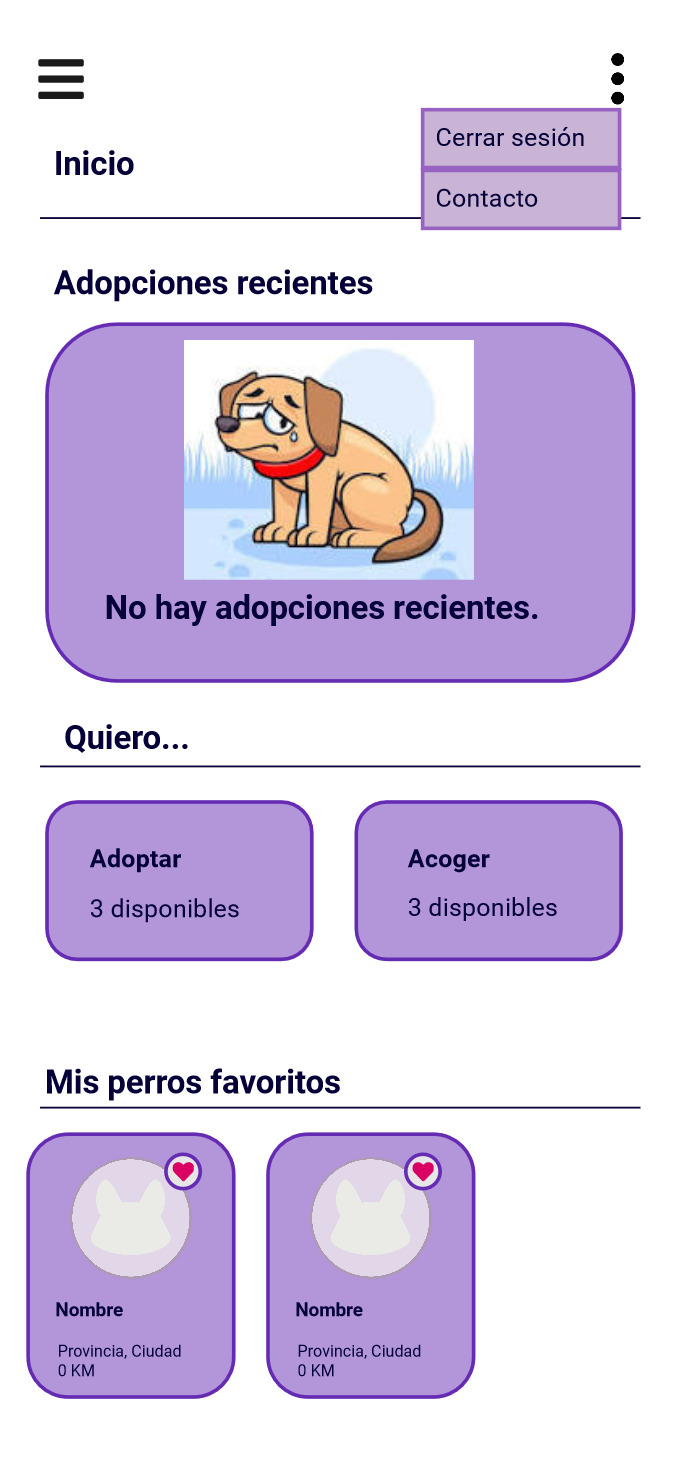
\includegraphics[height=8cm, width=4cm]{design/UserPage.jpg}\par}
			\caption{Pantalla de inicio de usuario.}
			\medskip
			\small

		\end{center}  
	\end{minipage}\hfill
   	\begin{minipage}{0.48\textwidth}
		\begin{center}
			{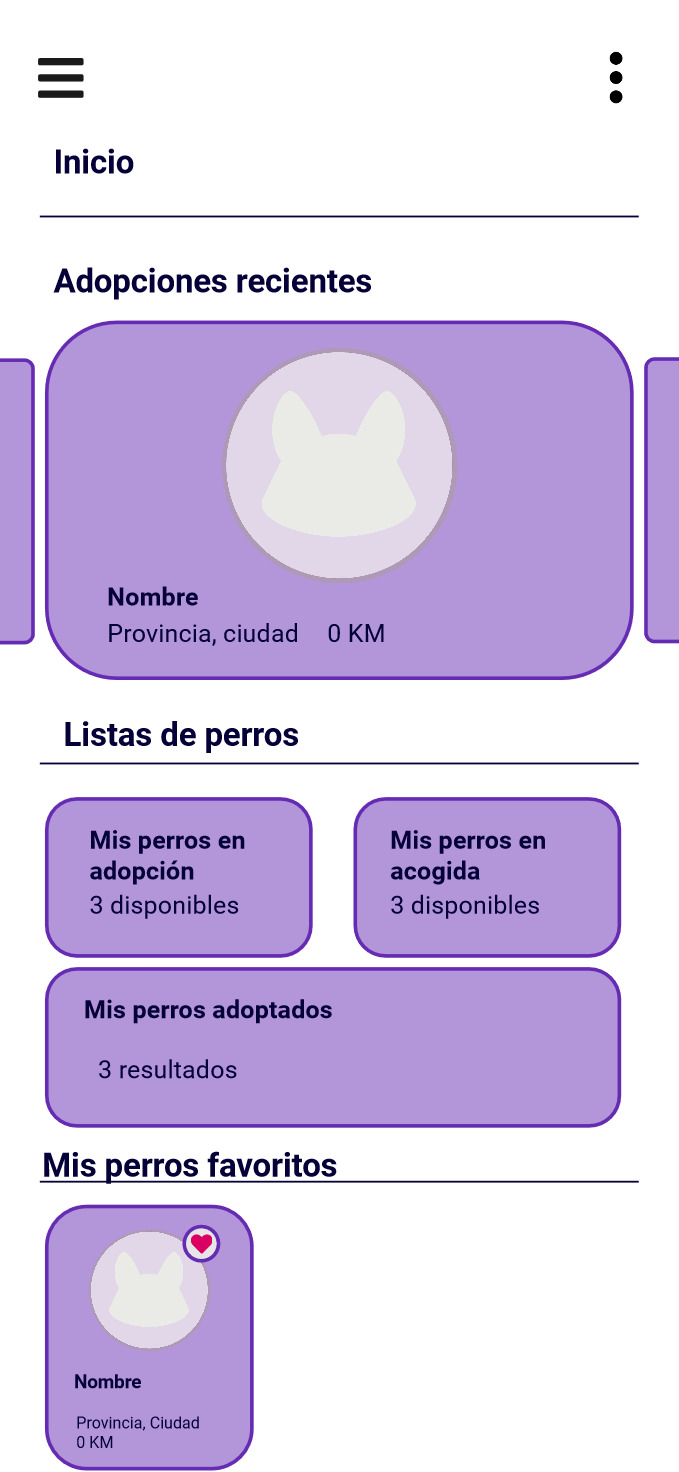
\includegraphics[height=8cm, width=4cm]{design/CompanyPage.jpg}\par}
			\caption{Pantalla de inicio para protectora.}
			\medskip			
		\end{center}  
	\end{minipage}\hfill
\end{figure}

\begin{figure}[H]
   	\begin{minipage}{0.48\textwidth}
		\begin{center}
			{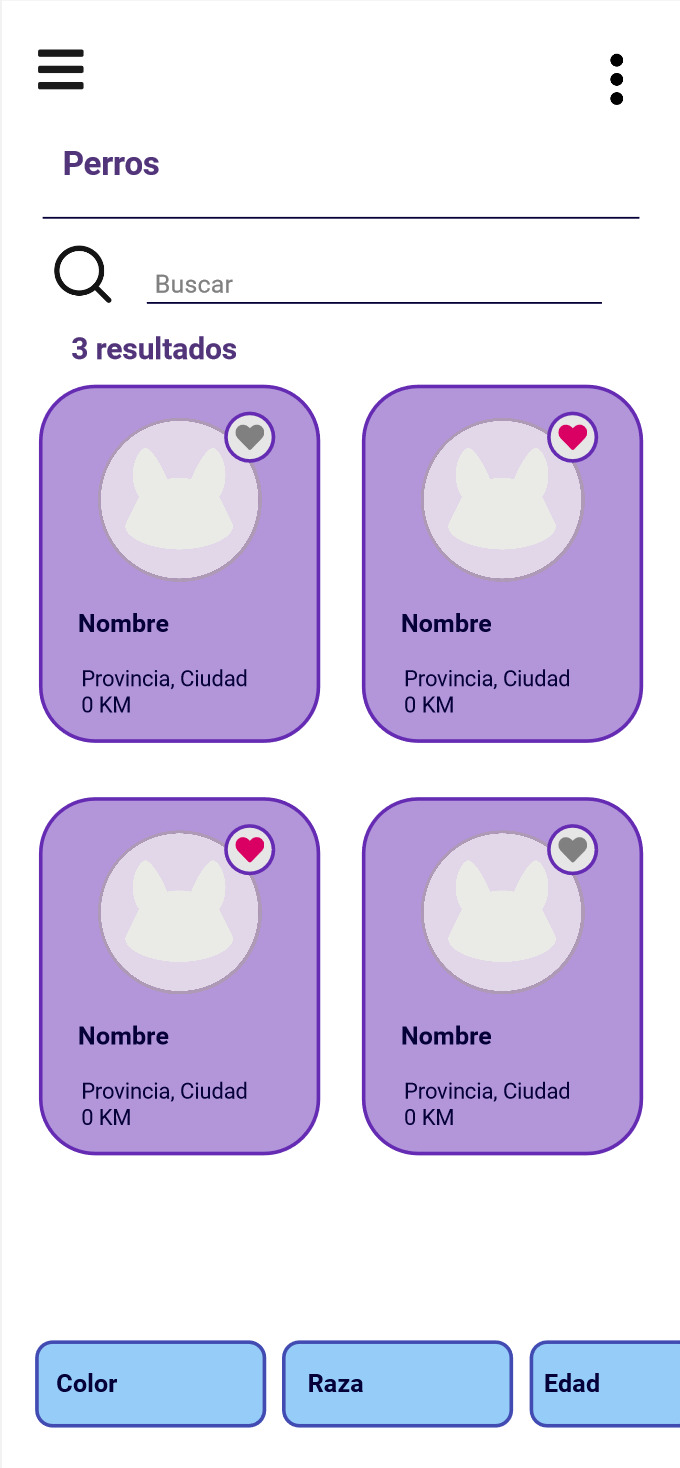
\includegraphics[height=8cm, width=4cm]{design/DogList.jpg}\par}
			\caption{Pantalla de lista de caninos.}
			\medskip
		\end{center}  
	\end{minipage}\hfill
   	\begin{minipage}{0.48\textwidth}
		\begin{center}
			{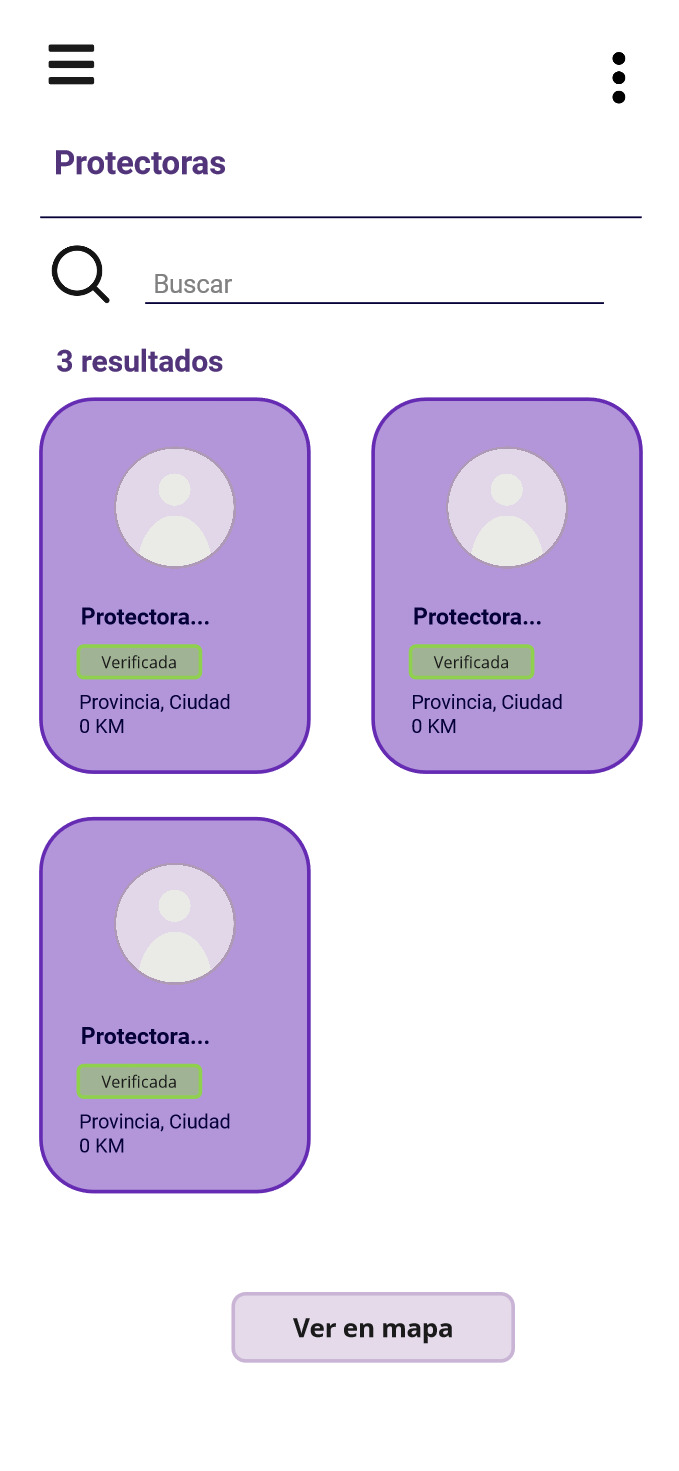
\includegraphics[height=8cm, width=4cm]{design/UserList.jpg}\par}
			\caption{Pantalla de lista de usuarios.}
			\medskip
		\end{center}  
	\end{minipage}\hfill
\end{figure}


\begin{figure}[H]
   	\begin{minipage}{0.48\textwidth}
		\begin{center}
			{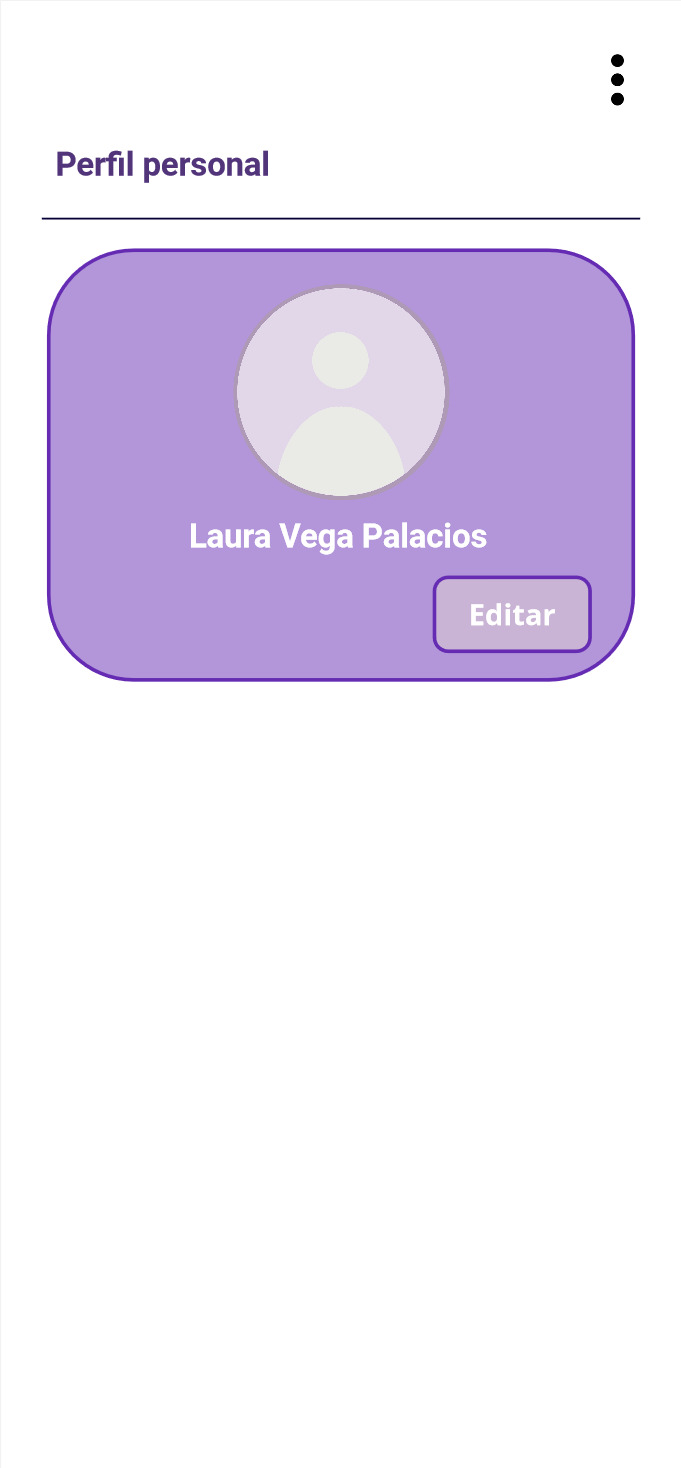
\includegraphics[height=8cm, width=4cm]{design/UserProfile.jpg}\par}
			\caption{Pantalla del perfil de usuario/administrador.}
			\medskip

		\end{center}  
	\end{minipage}\hfill
   	\begin{minipage}{0.48\textwidth}
		\begin{center}
			{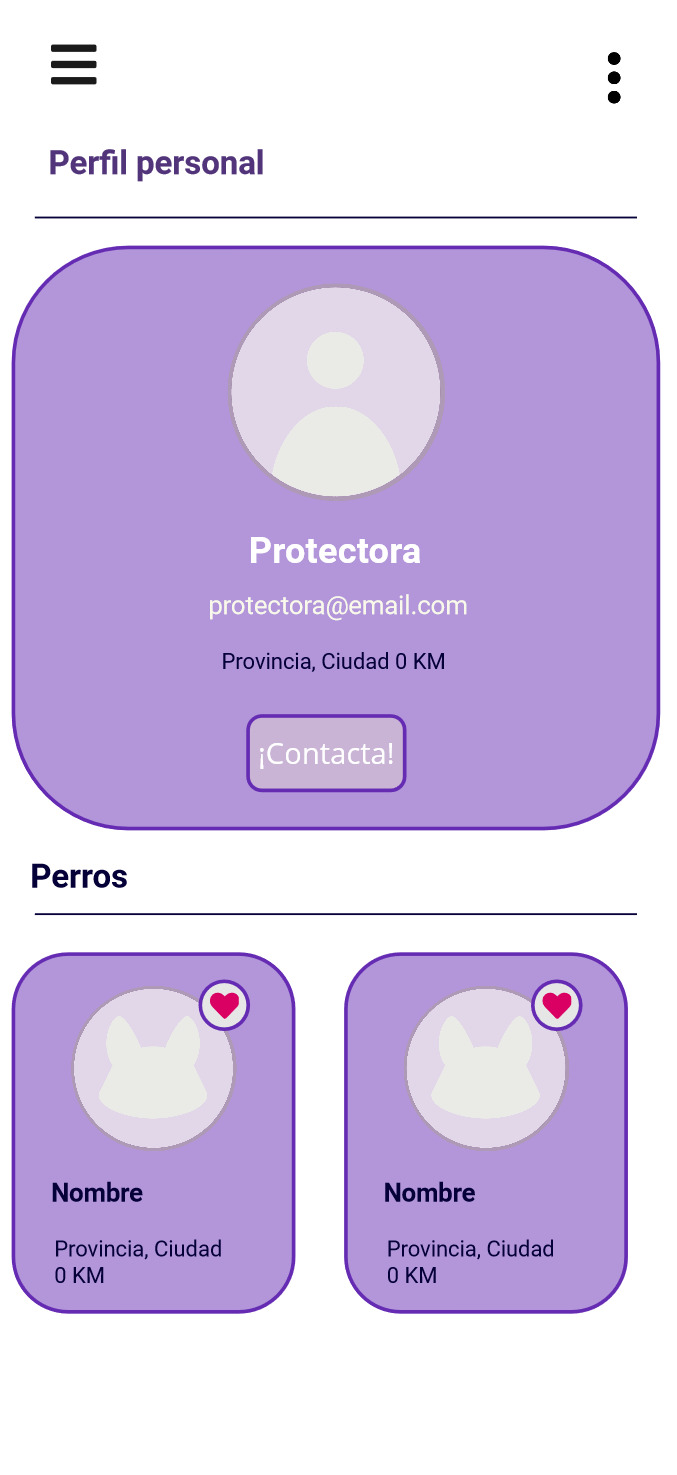
\includegraphics[height=8cm, width=4cm]{design/CompanyProfile.jpg}\par}
			\caption{Pnatalla del perfil de protectora. }
			\medskip
		\end{center}  
	\end{minipage}\hfill
\end{figure}

\begin{figure}[H]
   	\begin{minipage}{0.48\textwidth}
		\begin{center}
			{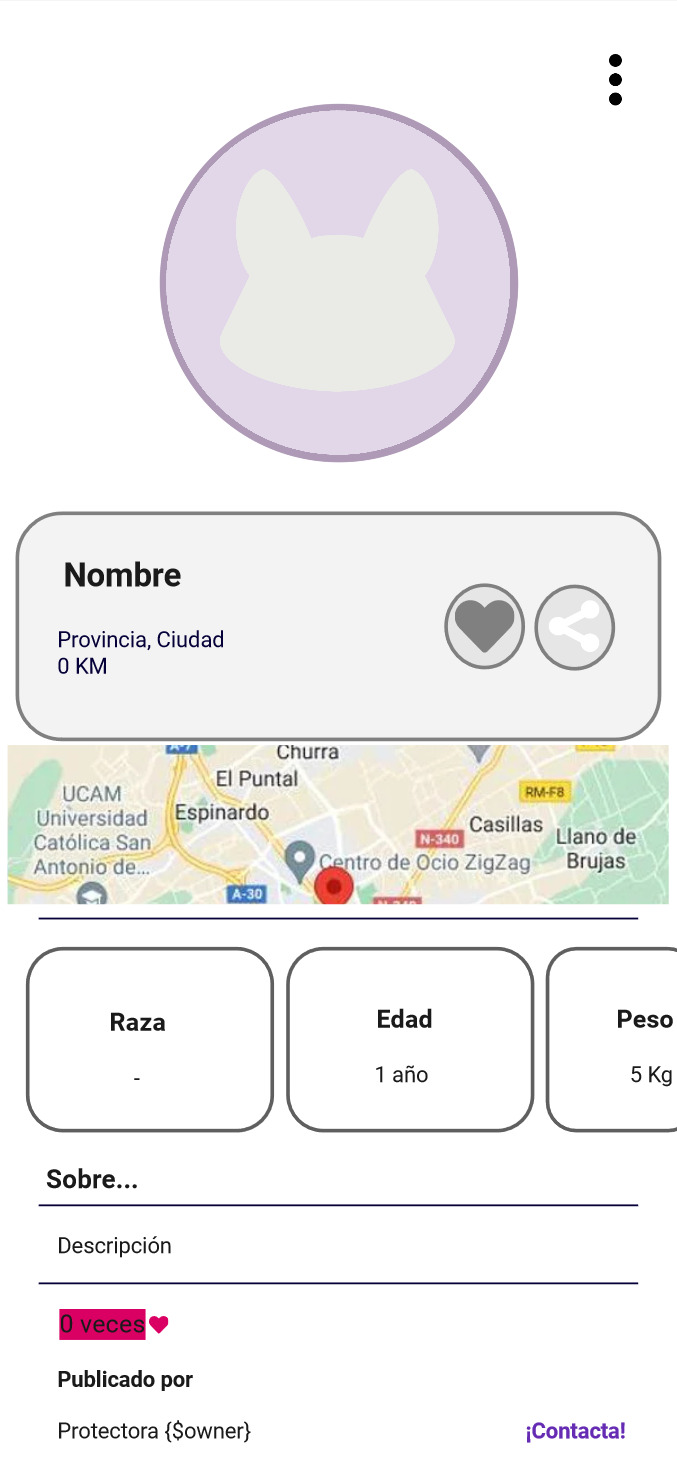
\includegraphics[height=8cm, width=4cm]{design/DogProfile.jpg}\par}
			\caption{Pantalla del perfil de canino.}
			\medskip
		\end{center}  
	\end{minipage}\hfill
   	\begin{minipage}{0.48\textwidth}
		\begin{center}
			{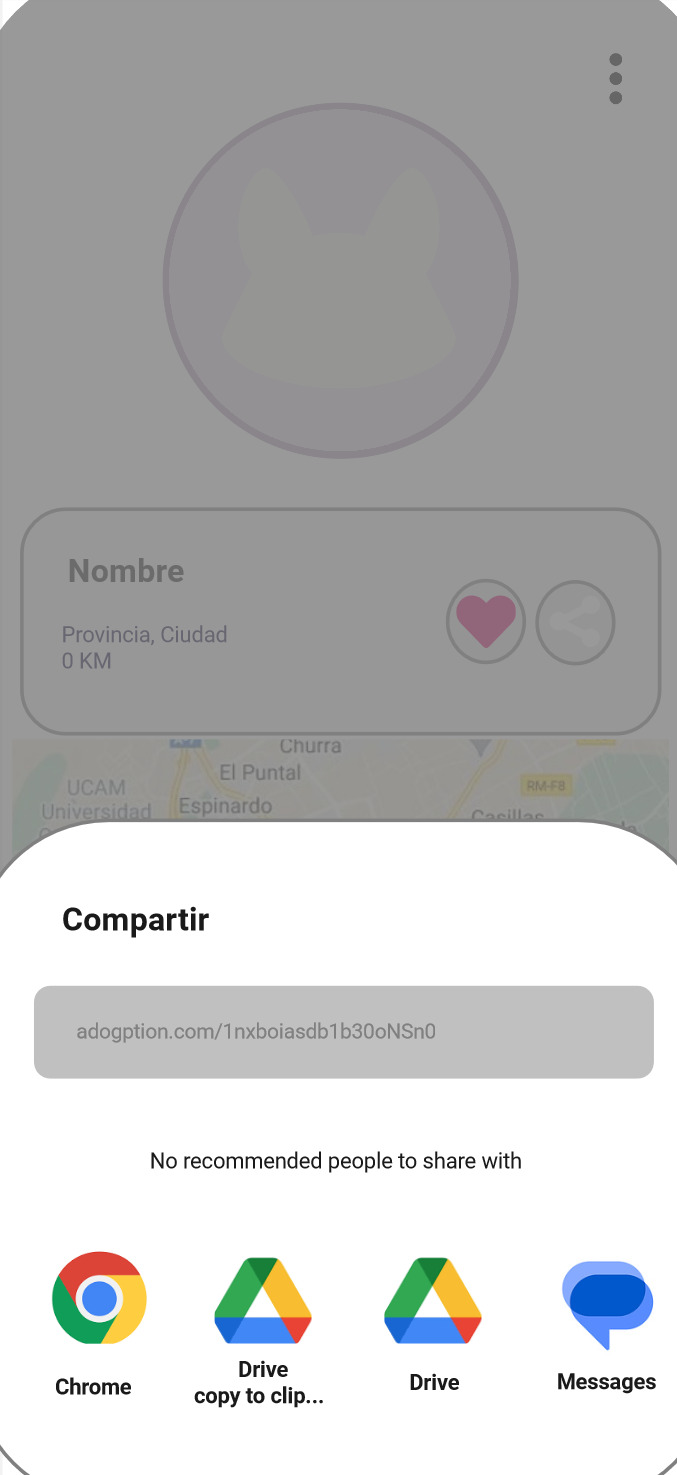
\includegraphics[height=8cm, width=4cm]{design/ShareAction.jpg}\par}
			\caption{Pantalla de compartir canino.}
			\medskip
		\end{center}  
	\end{minipage}\hfill
\end{figure}

\begin{figure}[H]
   	\begin{minipage}{0.48\textwidth}
		\begin{center}
			{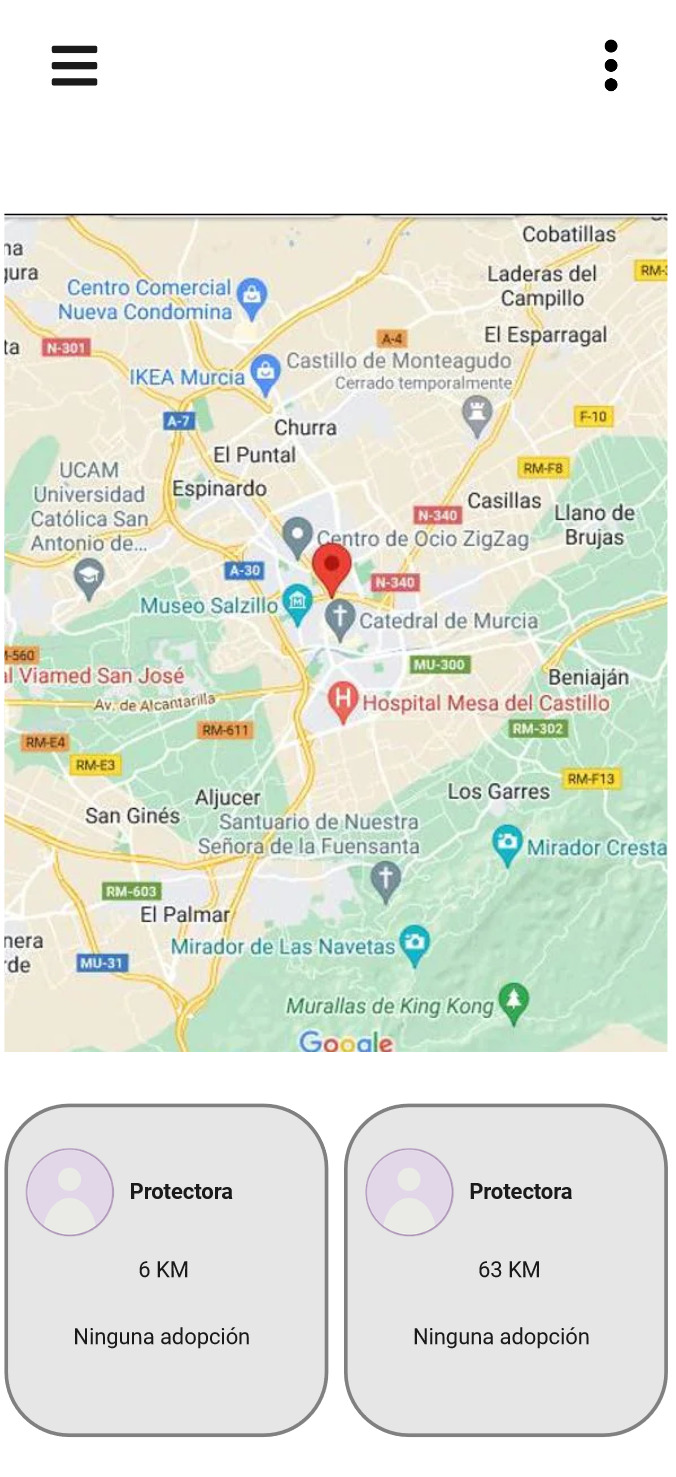
\includegraphics[height=8cm, width=4cm]{design/MapPage.jpg}\par}
			\caption{Pantalla de mapa y lista.}
			\medskip
		\end{center}  
	\end{minipage}\hfill
   	\begin{minipage}{0.48\textwidth}
		\begin{center}
			{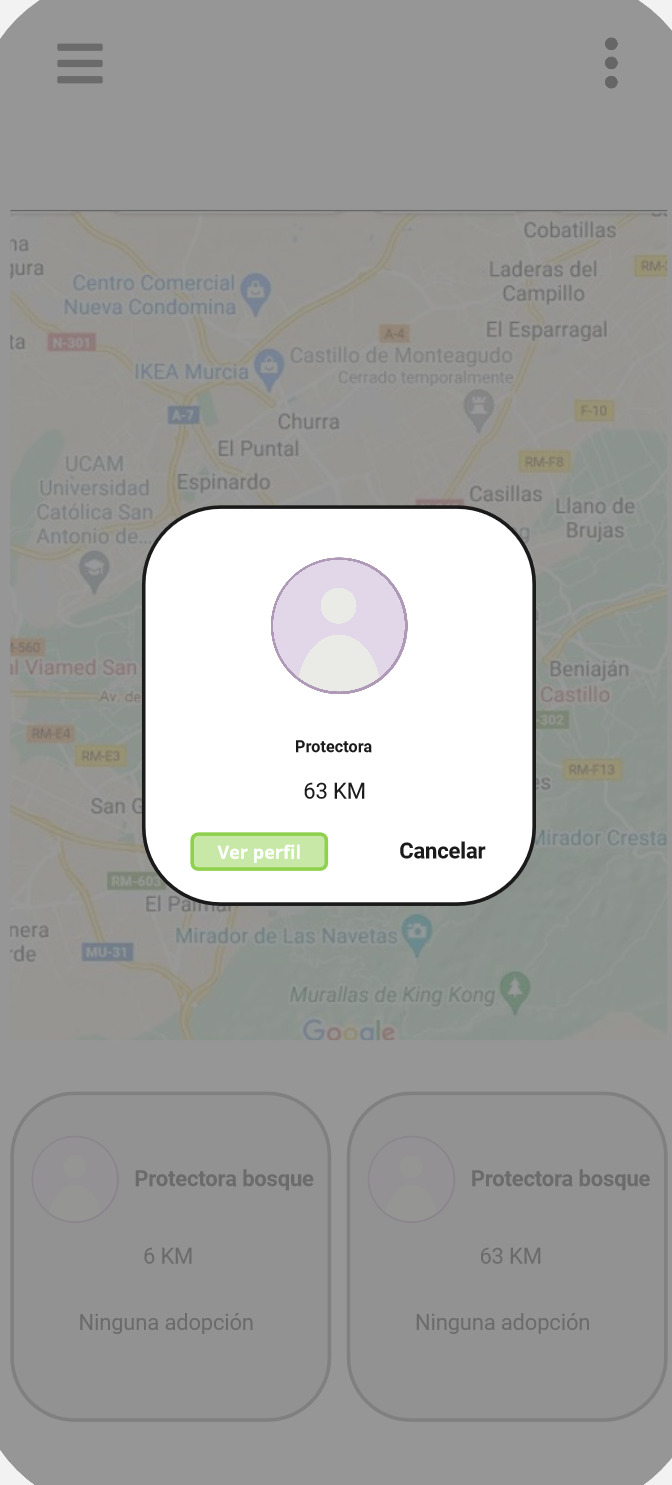
\includegraphics[height=8cm, width=4cm]{design/MapAction.jpg}\par}
			\caption{Pantalla de redirección a perfil.}
			\medskip
		\end{center}  
	\end{minipage}\hfill
\end{figure}

\begin{figure}[H]
   	\begin{minipage}{0.48\textwidth}
		\begin{center}
			{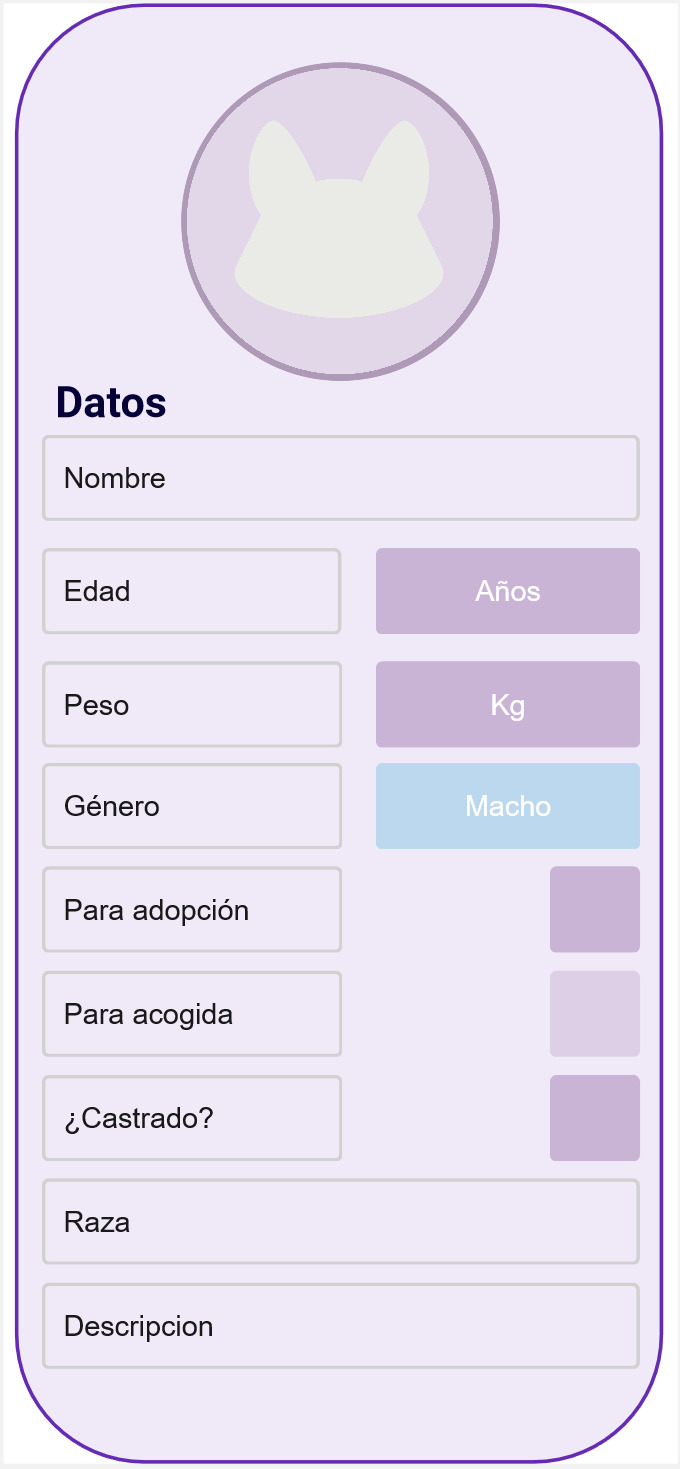
\includegraphics[height=8cm, width=4cm]{design/RegisterDog.jpg}\par}
			\caption{Pantalla de registro/edición de canino.}
			\medskip
		\end{center}  
	\end{minipage}\hfill
   	\begin{minipage}{0.48\textwidth}
		\begin{center}
			{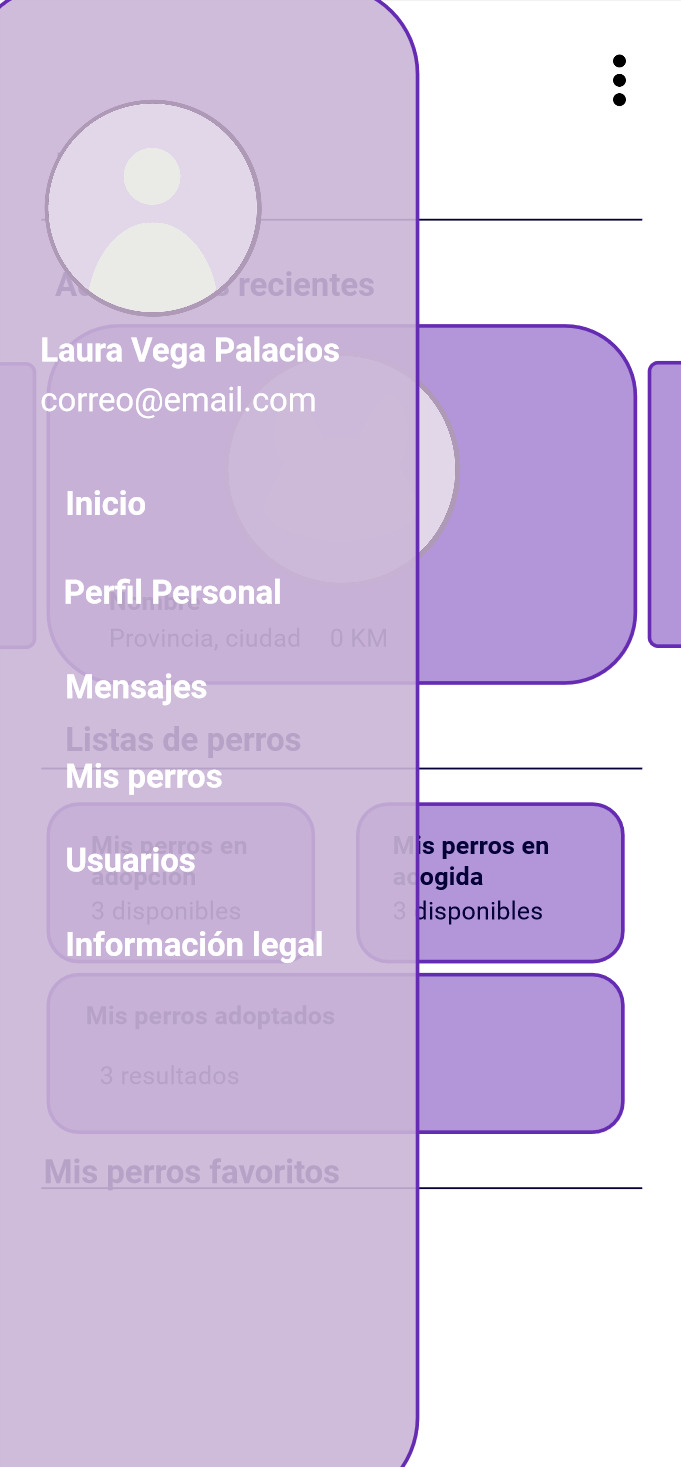
\includegraphics[height=8cm, width=4cm]{design/SideMenu.jpg}\par}
			\caption{Pantalla del menú.}
			\medskip
		\end{center}  
	\end{minipage}\hfill
\end{figure}

\begin{figure}[H]
   	\begin{minipage}{0.48\textwidth}
		\begin{center}
			{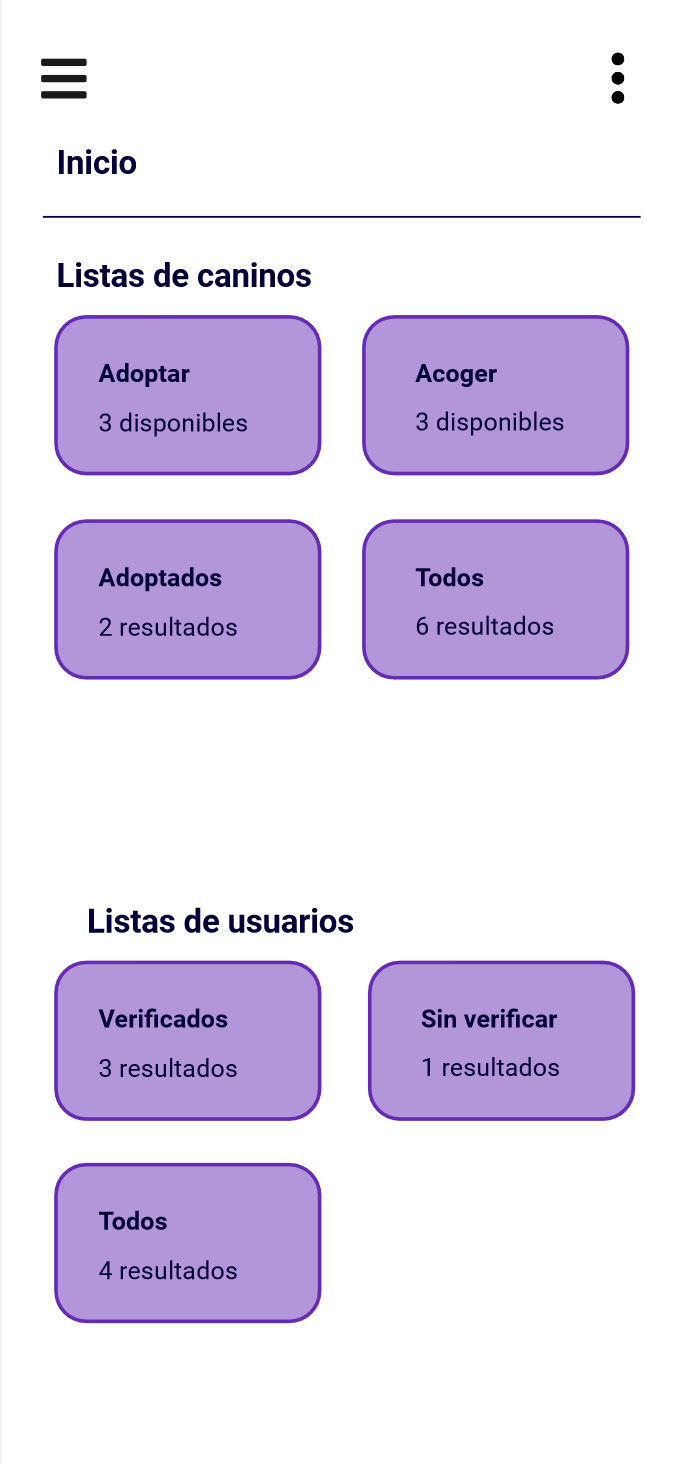
\includegraphics[height=8cm, width=4cm]{design/AdminPage.jpg}\par}
			\caption{Pantalla del inicio del administrador.}
			\medskip
		\end{center}  
	\end{minipage}\hfill
   	\begin{minipage}{0.48\textwidth}
		\begin{center}
			{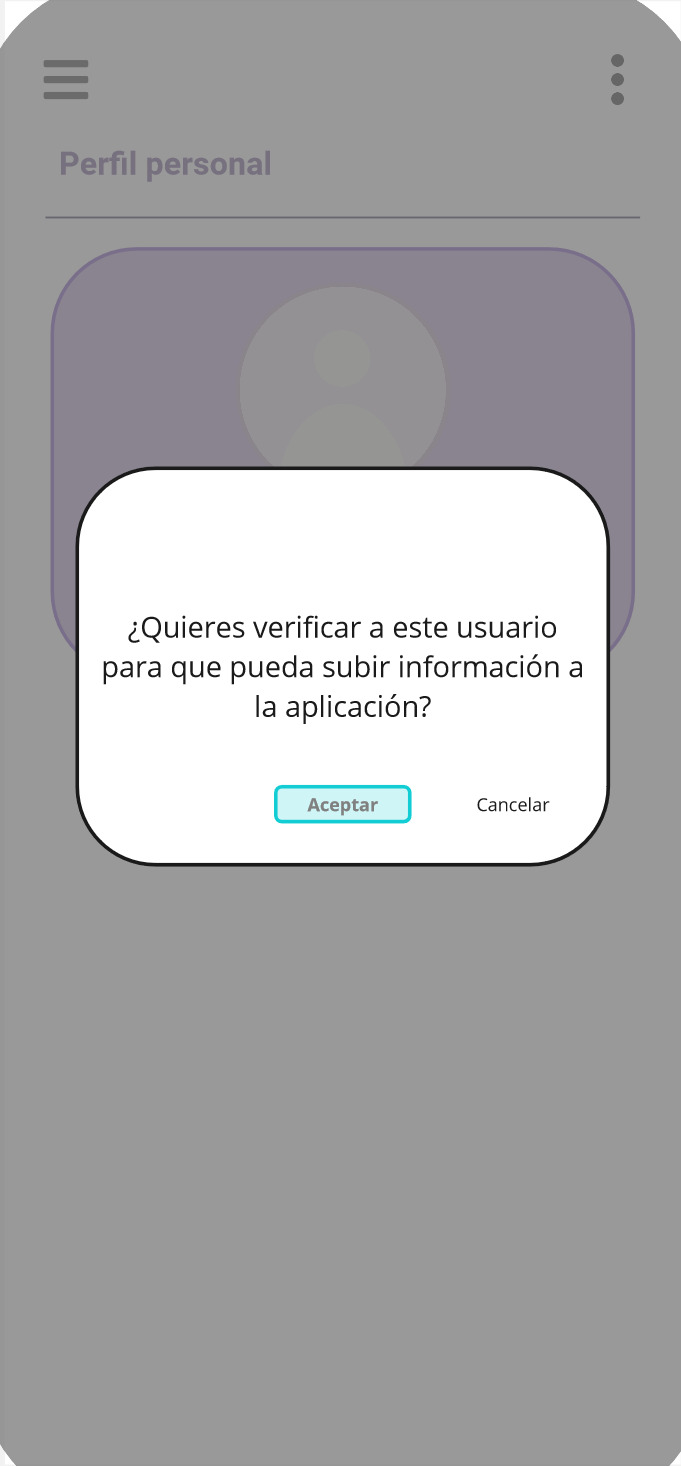
\includegraphics[height=8cm, width=4cm]{design/VerifyAction.jpg}\par}
			\caption{Pantalla del pop-up de verificación.}
			\medskip
		\end{center}  
	\end{minipage}\hfill
\end{figure}

\begin{figure}[H]
   	\begin{minipage}{0.48\textwidth}
		\begin{center}
			{
\includegraphics[height=8cm, width=4cm]{design/Notification.jpg}\par}
			\caption{Pantalla de notificaciones.}
			\medskip
		\end{center}  
	\end{minipage}\hfill
   	\begin{minipage}{0.48\textwidth}
		\begin{center}
			{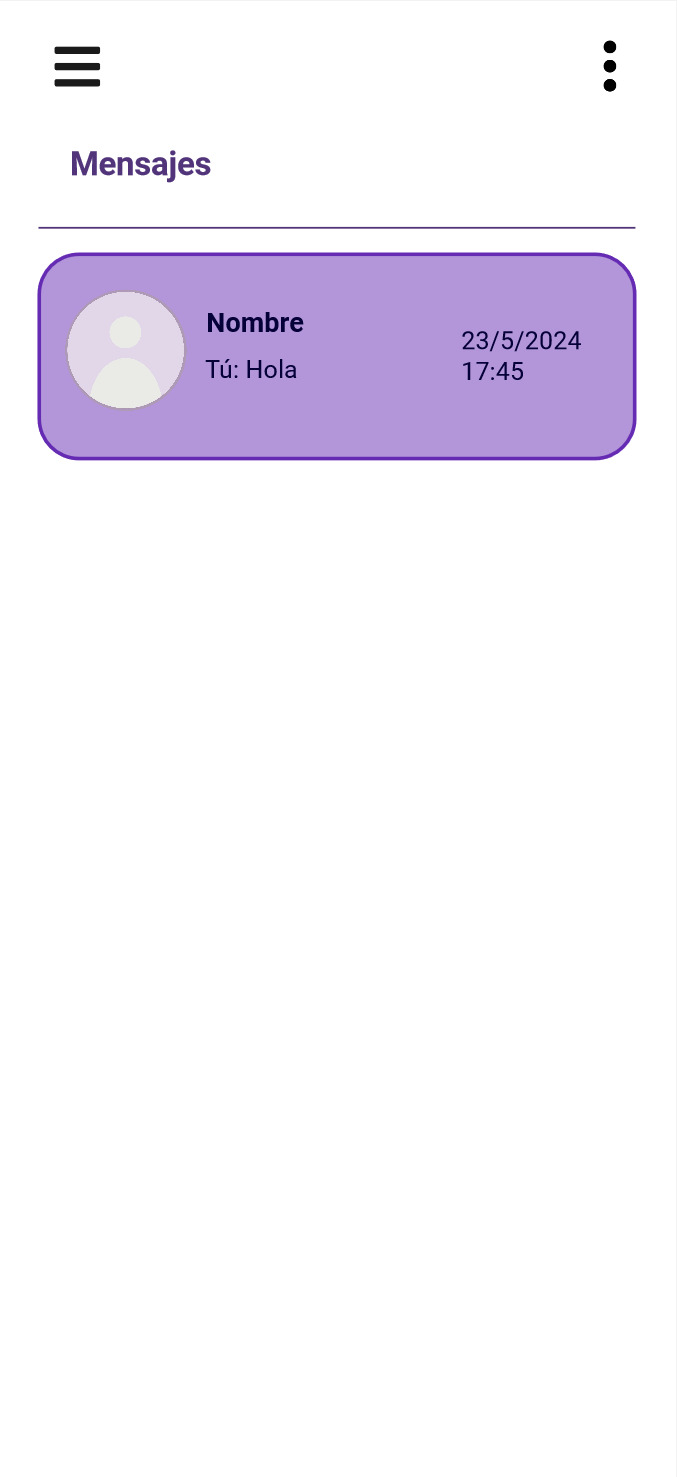
\includegraphics[height=8cm, width=4cm]{design/Messages.jpg}\par}
			\caption{Pantalla de chats.}
			\medskip
		\end{center}  
	\end{minipage}\hfill
\end{figure}

\begin{figure}[H]
   	\begin{minipage}{0.48\textwidth}
		\begin{center}
			{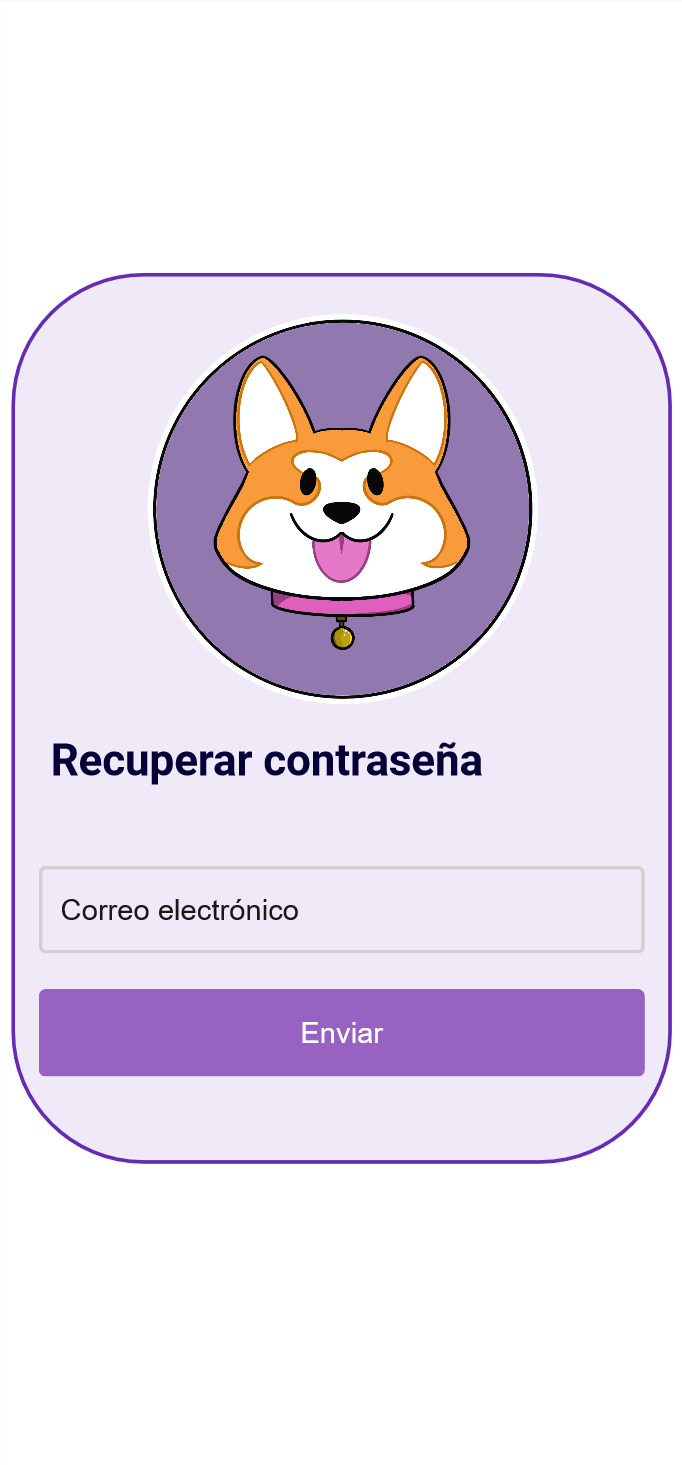
\includegraphics[height=8cm, width=4cm]{design/PasswordRecovery.jpg}\par}
			\caption{Pantalla de recuperación de contraseña.}
			\medskip
		\end{center}  
	\end{minipage}\hfill
\end{figure}


\subsection{Arquitectura interna}

Durante el desarrollo se han implementado diferentes módulos, cada uno con una finalidad específica. Mantener los componentes granulados en módulos y submódulos asegura una mejor escalabilidad y mantenibilidad de la aplicación y facilita tareas como refactorizaciones y cambios de estilos, además de evitar muchas repeticiones de código.


%Diagrama de modulos y sus dependencias
\begin{figure}[H]
	\begin{center}
		{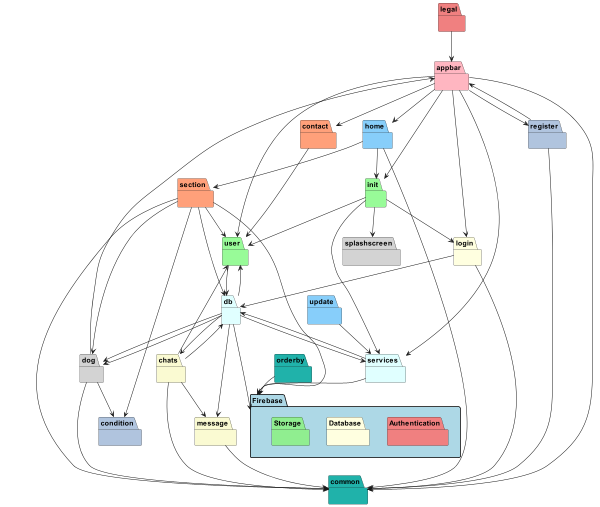
\includegraphics[width=13cm]{diagram/MODULES.png}\par}
		\caption{Módulos y sus dependencias.}
	\end{center}
\end{figure}


\newpage
\subsection*{appbar}


Este módulo se utiliza para generar las diferentes \textit{appbar} que se utilizan en las pantallas de la aplicación. Una \textit{appbar} es el componente que se coloca en la parte superior de la pantalla y puede contener botones u otros componentes tales como barras de búsqueda o imágenes. La única clase que contiene el módulo se encarga de instanciar el componente en las diferentes pantallas según el tipo de barra que se necesite.

\begin{figure}[H]
	\begin{center}
		{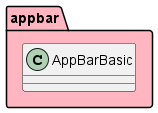
\includegraphics[]{diagram/AppBar.png}\par}
		\caption{Módulo \textit{appbar}.}
	\end{center}
\end{figure}


\subsection*{chats}

En este módulo se incluyen todas las clases que necesita un chat para funcionar correctamente:
\begin{itemize}[noitemsep]
	\item \textbf{ChatInput}: componente que permite a los usuarios escribir mensajes y adjuntar imágenes a los chats.
	\item \textbf{ChatRoomPage}: interfaz del chat.
	\item \textbf{ChatsPage}:  es la página principal que contiene todos los chats. Contiene todos los chats que un usuario tiene en ese momento, son una lista de \textit{ChatWidget}.
	\item \textbf{ChatWidget}: este componente muestra una previsualización del chat, que incluye la información del usuario, el último mensaje y la fecha y hora en la que se envió. Además, incluye el número de mensajes sin leer del chat.
	\item \textbf{ChatModel}: clase que se encarga de manejar modelos de chat que se generan a partir de toda la información de la base de datos relacionada con ellos.
\end{itemize}

\begin{figure}[H]
	\begin{center}
		{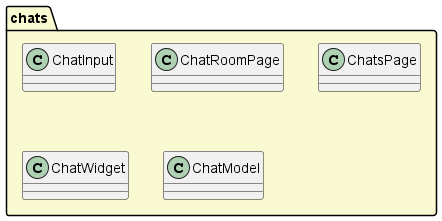
\includegraphics[width=0.7\linewidth]{diagram/Chats.png}\par}
		\caption{Módulo \textit{chats}.}
	\end{center}
\end{figure}


\subsection*{common}

En este módulo se definen todos los componentes básicos que incluyen las diferentes pantallas generadas. Además, se definen diferentes submódulos para cada uno de los componentes creados. Los submódulos contienen una clase base en la que se definen los estilos y funcionalidades básicas, y el resto de las clases extienden de estas clases base. Es importante destacar que, aunque se hayan creado clases propias para los componentes, todas ellas instancian componentes de las bibliotecas por defecto de Flutter, como la biblioteca \textit{material}. Sus clases son las siguientes:

\begin{itemize}[noitemsep]
	\item \textbf{button}: en este submódulo se definen todos los botones utilizados en diversos componentes y pantallas de la aplicación. Estos botones tienen diferentes funcionalidades, como la redirección a otras pantallas, la actualización de datos o la visualización de pop-ups.
	\item \textbf{card}: una tarjeta es un componente similar a un contenedor pero con un aspecto más atractivo. Se ha creado un componente base que se reutiliza en diferentes widgets y que contiene este módulo.
	\item \textbf{checkbox}: contiene los diferentes checkboxes desarrollados, junto con su comportamiento asociado.
	\item \textbf{container}: define un contenedor básico con un estilo concreto para reutilizarlo en diferentes lugares.
	\item \textbf{dialog}: agrupa todos los pop-ups desarrollados y su comportamiento correspondiente.
	\item \textbf{drawer}: contiene todos los menús laterales y los componentes asociados. Estos menús incluyen imágenes de perfil y botones que redirigen a otras pantallas.
	\item \textbf{dropdown}: incluye los diferentes dropdowns utilizados en la aplicación. Algunos de los cuales tienen la funcionalidad de búsqueda de opciones.
	\item \textbf{form}: contiene todos los formularios utilizados en la aplicación.
	\item \textbf{icon}: agrupa iconos básicos con funcionalidad. Por ahora, solo incluye el icono de favoritos.
	\item \textbf{images}: incluye clases que proporcionan funcionalidades para seleccionar imágenes del dispositivo y componentes para facilitar la inserción de imágenes en la aplicación.
	\item \textbf{input}: contiene componentes que permiten a los usuarios introducir información de diversos tipos, como texto, números o componentes compuestos que contienen dropdowns o checkboxes.
	\item \textbf{maps}: incluye toda la funcionalidad relacionada con los mapas, es decir, tanto la página de mapas como los mapas que se pueden insertar en diferentes partes de la aplicación.
	\item \textbf{padding}: define un \textit{padding} que se reutiliza en toda la aplicación.
	\item \textbf{picker}: incluye componentes relacionados con la selección de direcciones en mapas u opciones similares.
	\item \textbf{searchbar}: define las barras de búsqueda implementadas en la aplicación junto con su funcionalidad.
	\item \textbf{swiper}: contiene el swiper utilizado para mostrar las adopciones recientes.
	\item \textbf{text}: contiene clases que definen textos utilizados en la aplicación, como títulos, subtítulos y avisos.
	\item \textbf{widget}: incluye componentes comunes compuestos por otros componentes comunes.
\end{itemize}


\begin{figure}[H]
	\begin{center}
		{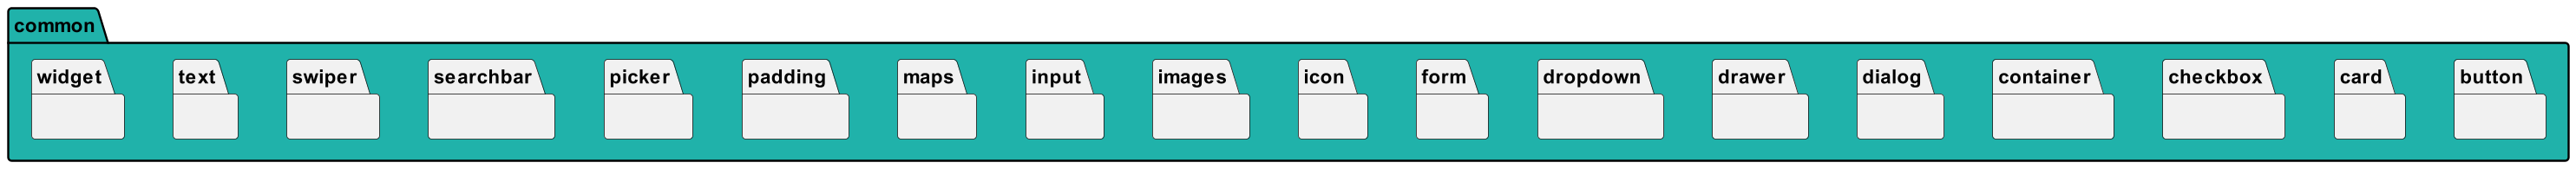
\includegraphics[width=0.8\linewidth]{diagram/Common.png}\par}
		\caption{Módulo  \textit{common}.}
	\end{center}
\end{figure}

\subsection*{condition}

Este módulo se encarga de gestionar los filtros de las listas de una manera más dinámica. Sus clases son las siguientes:

\begin{itemize}[noitemsep]
	\item \textbf{Basic}: define el componente básico para añadir filtros a las listas, encargándose de abrir el pop-up con las opciones del filtro.
	\item \textbf{Gender}: define el filtro para el género.
	\item \textbf{Weight}: define el filtro para el peso.
	\item \textbf{ConditionModel}: clase que se encarga de generar y manejar modelos de condiciones a partir de la información proporcionada por la aplicación o el usuario. Esta clase, además, proporciona un método que se encarga de añadir todos los filtros que haya aplicados en ese momento a la consulta.
\end{itemize}

\begin{figure}[H]
	\begin{center}
		{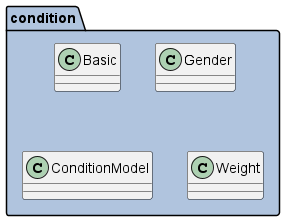
\includegraphics[]{diagram/Condition.png}\par}
		\caption{Módulo \textit{condition}.}
	\end{center}
\end{figure}

\subsection*{contact}

Aunque este módulo solo contiene una clase que se encarga de mostrar toda la información de contacto con los administradores, se ha definido por separado para poder añadir más clases en un futuro.

\begin{figure}[H]
	\begin{center}
		{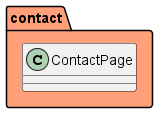
\includegraphics[]{diagram/Contact.png}\par}
		\caption{Módulo \textit{contact}.}
	\end{center}
\end{figure}


\subsection*{db}

Este módulo es el encargado de comunicarse directamente con la base de datos de Firebase. Contiene diferentes clases para las distintas entidades que existen y para el almacenamiento:

\begin{itemize}[noitemsep]
	\item \textbf{DBBase}: contiene los métodos básicos que deben incluir el resto de clases.
	\item \textbf{DBAddresses}: maneja las direcciones y coordenadas.
	\item \textbf{DBChats}: maneja toda la información relacionada con chats.
	\item \textbf{DBDogs}: maneja toda la información relacionada con caninos y su información.
	\item \textbf{DBFavorites}: se encarga exclusivamente de actualizar la información de los favoritos dentro de la tabla de caninos.
	\item \textbf{DBMessages}: maneja toda la información relacionada con mensajes.
	\item \textbf{DBNotifications}: maneja toda la información relacionada con notificaciones.
	\item \textbf{DBStorage}: se encarga de insertar, actualizar y eliminar todas las imágenes relacionadas con alguna de las entidades.
	\item \textbf{DBUsers}: maneja toda la información relacionada con los usuarios.
\end{itemize}

\begin{figure}[H]
	\begin{center}
		{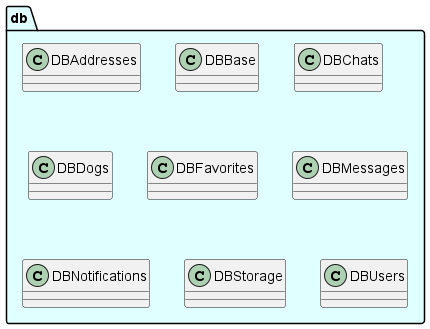
\includegraphics[width=0.7\linewidth]{diagram/DB.png}\par}
		\caption{Módulo  \textit{db}.}
	\end{center}
\end{figure}


\subsection*{dog}

Módulo que contiene las clases principales relacionadas con los caninos. Sus clases son las siguientes:

\begin{itemize}[noitemsep]
	\item \textbf{AvailableDogsPage}: pantalla de lista de caninos que contiene los filtros y una barra de búsqueda. Se encarga de manejar las consultas y mostrar los resultados.
	\item \textbf{DogFeature}: widget que se instancia con la información de alguno de los atributos del canino para mostrarlo en el perfil.
	\item \textbf{DogProfile}: pantalla que contiene toda la información de un canino, incluyendo el botón de favoritos y compartir.
	\item \textbf{DogModel}: clase que se encarga de generar y manejar modelos de caninos a partir de la información en la base de datos.
\end{itemize}

\begin{figure}[H]
	\begin{center}
		{\includegraphics[width=0.8\linewidth]{diagram/Dog.png}\par}
		\caption{Módulo  \textit{dog}.}
	\end{center}
\end{figure}


\subsection*{home}

Incluye todas las pantallas de inicio definidas para los diferentes roles. Sus clases son las siguientes:

\begin{itemize}[noitemsep]
	\item \textbf{AdminHome}: pantalla de inicio para administradores.
	\item \textbf{MyHome}: pantalla de inicio para usuarios.
	\item \textbf{MyHomePageCompany}: pantalla de inicio para protectoras.
\end{itemize}

\begin{figure}[H]
	\begin{center}
		{\includegraphics[width=0.8\linewidth]{diagram/Home.png}\par}
		\caption{Módulo  \textit{home}.}
	\end{center}
\end{figure}


\subsection*{init}

La clase contenida en este módulo se encarga de manejar la pantalla que se debe mostrar cuando se abre la aplicación, además de inicializar todos los servicios que lo requieran. La pantalla mostrará la pantallla de carga y, dependiendo de si hay un usuario iniciado, se redigirá a la pantalla de inicio del rol correspondiente o a la pantalla de inicio de sesión.

\begin{figure}[H]
	\begin{center}
		{\includegraphics[]{diagram/Init.png}\par}
		\caption{Módulo  \textit{init}.}
	\end{center}
\end{figure}


\subsection*{legal}

Este módulo solo contiene una pantalla que contiene toda la información legal relacionada con las adopciones y los usos de la aplicación.

\begin{figure}[H]
	\begin{center}
		{\includegraphics[]{diagram/Legal.png}\par}
		\caption{Módulo  \textit{legal}.}
	\end{center}
\end{figure}


\subsection*{login}


Este módulo contiene la página para iniciar sesión y la de recuperación de contraseña.

\begin{figure}[H]
	\begin{center}
		{\includegraphics[width=0.8\linewidth]{diagram/Login.png}\par}
		\caption{Módulo  \textit{login}.}
	\end{center}
\end{figure}


\subsection*{message}

En este módulo se definen los widgets relacionados con los mensajes que se utilizan dentro de las salas de chat. Sus clases son las siguientes:

\begin{itemize}[noitemsep]
	\item \textbf{DateMessageDivider}: este widget se coloca entre mensajes de días diferentes para indicar la fecha de los mensajes siguientes.
	\item \textbf{MessageWidget}: este widget muestra el contenido del mensaje, que puede ser texto o imagen, y también incluye un icono que indica si el mensaje ha sido leído o no.
	\item \textbf{MessageModel}: clase que se encarga de generar y manejar modelos de mensajes a partir de la información en la base de datos.
\end{itemize}


\begin{figure}[H]
	\begin{center}
		{\includegraphics[width=0.8\linewidth]{diagram/Message.png}\par}
		\caption{Módulo \textit{message}.}
	\end{center}
\end{figure}


\subsection*{orderby}

Este módulo contiene el modelo para añadir la cláusula de orden a las consultas.

\begin{figure}[H]
	\begin{center}
		{\includegraphics[]{diagram/OrderBy.png}\par}
		\caption{Módulo  \textit{orderby}.}
	\end{center}
\end{figure}


\subsection*{register}

Este módulo todas las páginas relacionadas con los registros dentro de la app. Cada una de las pantallas incluye un formulario específico que se encarga de todas las validaciones. Sus clases son las siguientes:

\begin{itemize}[noitemsep]
	\item \textbf{RegisterAsCompanyPage}: pantalla de registro de protectora.
	\item \textbf{RegisterAsUserPage}: pantalla de registro de usuario.
	\item \textbf{RegisterDog}: pantalla de registro de canino.
	\item \textbf{RegisterPage}:  pantalla que ofrece las opciones para registrarse como protectora o usuario.
\end{itemize}

\begin{figure}[H]
	\begin{center}
		{\includegraphics[width=0.8\linewidth]{diagram/Register.png}\par}
		\caption{Módulo  \textit{register}.}
	\end{center}
\end{figure}

\subsection*{section}

Este módulo contiene diferentes widgets que definen secciones que se reutilizan en algunas de las pantallas. Sus clases son las siguientes:

\begin{itemize}[noitemsep]
	\item \textbf{AdminCategorySection}: incluye la sección principal de la página de inicio de administrador.
	\item \textbf{CompanyCategorySection}: incluye la sección principal de la página de inicio de protectora.
	\item \textbf{RecentAdoptionsSection}:  define la sección de adopciones recientes que se usa en diferentes páginas de inicio.
	\item \textbf{UserCategorySection}:  incluye la sección principal de la página de inicio de usuario.
	\item \textbf{UserFavoritesSection}:  define la sección de favoritos de un usuario específico.
	\item \textbf{UserOwnedDogsSection}:  define la sección de caninos que son de un usuario específico.
\end{itemize}


\begin{figure}[H]
	\begin{center}
		{\includegraphics[width=0.8\linewidth]{diagram/Section.png}\par}
		\caption{Módulo  \textit{section}.}
	\end{center}
\end{figure}


\subsection*{services}

En este módulo, se incluyen clases que manejan los servicios que proporciona Flutter o Firebase además de otras clases que son servicios creados específicamente para la aplicación. Sus clases son las siguientes:

\begin{itemize}[noitemsep]
	\item \textbf{AddressService}: servicio para manejar los modelos de las direcciones y las coordenadas.
	\item \textbf{AwesomeNotificationService}: clase que maneja el servicio de notificaciones. 
	\item \textbf{GeocodingService}: clase que maneja el servicio de \textit{geocoding} que proporciona Google dentro de la app.
	\item \textbf{RoutingService}:  servicio para manejar las rutas de la aplicación.
	\item \textbf{Auth - AuthUsers}:  clase que maneja el servicio de autenticación que proporciona Firebase.
\end{itemize}



\begin{figure}[H]
	\begin{center}
		{\includegraphics[width=0.8\linewidth]{diagram/Services.png}\par}
		\caption{Módulo  \textit{services}.}
	\end{center}
\end{figure}

\subsection*{update}

Este módulo contiene las páginas que incluyen formularios para la actualización de datos de usuarios y de caninos.

\begin{figure}[H]
	\begin{center}
		{\includegraphics[]{diagram/Update.png}\par}
		\caption{Módulo  \textit{update}.}
	\end{center}
\end{figure}



\subsection*{user}

Módulo que contiene todas las clases relacionadas con los usuarios y protectoras. Sus clases son las siguientes:

\begin{itemize}[noitemsep]
	\item \textbf{CurrentUser}: clase \textit{singleton} que se encarga de manejar todos los datos relacionados con el usuario iniciado a lo largo de la aplicación.
	\item \textbf{LoggedUserModel}: clase para manejar el modelo del usuario iniciado.
	\item \textbf{UserModel}: clase que se encarga de generar y manejar modelos de usuarios a partir de la información en la base de datos. 
	\item \textbf{ProfilePage}:  pantalla que contiene toda la información personal del usuario. Puede contener un listado de caninos y un botón para abrir una página de mapa dependiendo del rol de usuario.
	\item \textbf{UserMapWidget}: elemento que se instancia en las listas usadas en los mapas con toda la información del usuario.
	\item \textbf{UsersPage}: pantalla de la lista de usuarios que contiene además la barra de búsqueda. Se encarga de manejar las consultas y mostrar los resultados.
\end{itemize}

\begin{figure}[H]
	\begin{center}
		{\includegraphics[width=0.8\linewidth]{diagram/User.png}\par}
		\caption{Módulo  \textit{user}.}
	\end{center}
\end{figure}

% Implementación
\newpage
\section{Aspecto final de la aplicación}

En esta sección se incluyen las pantallas tras finalizar el proceso de desarrollo.

%Splashscreen
\subsection*{Pantalla de carga}

La pantalla de carga es una pantalla de transición que se utiliza justo después de iniciar sesión, mientras se carga toda la información del usuario.

\begin{figure}[H]
	\begin{center}
		{\includegraphics[width=5cm]{app/Splashscreen.png}\par}
		\caption{Pantalla de carga.}
	\end{center}
\end{figure}


%Login
\newpage
\subsection*{Inicio de sesión}

La pantalla de inicio de sesión muestra un formulario básico para introducir el correo electrónico y la contraseña. Este formulario indicará si hay errores durante el intento de iniciar sesión. El botón de inicio de sesión maneja toda la autenticación mediante el servicio de autenticación de Firebase.

\begin{figure}[H]
   	\begin{subfigure}{0.48\textwidth}
		\begin{center}
			{\includegraphics[width=5cm]{app/Login.png}\par}
			\caption{Aspecto normal.}
		\end{center}  
	\end{subfigure}\hfill
   	\begin{subfigure}{0.48\textwidth}
		\begin{center}
			{\includegraphics[width=5cm]{app/LoginWithErrors.png}\par}
			\caption{Aspecto con errores.}
		\end{center}  
	\end{subfigure}\hfill
	\caption{Pantalla de inicio de sesión.}\label{fig:login}
\end{figure}



%Recover password
\newpage
\subsection*{Recuperación de contraseña}

Esta pantalla contiene un formulario que solo incluye un campo para introducir el correo electrónico. Si el éste está registrado, el servicio de autenticación de Firebase se encargará de enviar al usuario, protectora o administrador un correo electrónico con las instrucciones para cambiar la contraseña.

\begin{figure}[H]
	\begin{center}
		{\includegraphics[width=5cm]{app/RecoverPassword.png}\par}
		\caption{Pantalla de recuperación de contraseña.}
	\end{center}
\end{figure}

%Register
\newpage
\subsection*{Registro}

Si se pulsa el botón \textit{Regístrate} que se incluye en la pantalla de inicio de sesión mostrada en la Figura \ref{fig:login}, se redirige a una pantalla que muestran dos botones que llevan a los formularios para registrarse como usuario normal o como protectora respectivamente. Ambos formularios de registro piden los mismos datos a excepción de la dirección, que solo se requiere en el caso de las protectoras.

\begin{figure}[H]
	\begin{center}
		{\includegraphics[width=5cm]{app/Register.png}\par}
		\caption{Pantalla de opciones de registro.}
	\end{center}  
\end{figure}

\begin{figure}[H]
   	\begin{subfigure}{0.48\textwidth}
		\begin{center}
			{\includegraphics[width=5cm]{app/RegisterUserEmpty.png}\par}
			\caption{Registro como usuario.}
		\end{center}  
	\end{subfigure}\hfill
   	\begin{subfigure}{0.48\textwidth}
		\begin{center}
			{\includegraphics[width=5cm]{app/RegisterCompanyAddress.png}\par}
			\caption{Registro como protectora.}
		\end{center}  
	\end{subfigure}\hfill
	\caption{Pantallas de registro.}
\end{figure}


\begin{figure}[H]
   	\begin{subfigure}{0.48\textwidth}
		\begin{center}
			{\includegraphics[width=5cm]{app/RegisterUserError.png}\par}
			\caption{Formulario base.}
		\end{center}  
	\end{subfigure}\hfill
   	\begin{subfigure}{0.48\textwidth}
		\begin{center}
			{\includegraphics[width=6cm]{app/AddressError.png}\par}
			\caption{Formulario de dirección con errores.}
		\end{center}  
	\end{subfigure}\hfill
	\caption{Pantallas de registro con errores.}
\end{figure}


El componente más complejo de estos formularios es la barra de búsqueda de direcciones. Este componente se ha desarrollado en base a otro proporcionado por el paquete \textit{search\_map\_location} \cite{search_map_location}, que incluye la funcionalidad básica para buscar direcciones con la API de Google Maps. A este componente se le ha añadido el comportamiento de autocompletar los campos del formulario una vez seleccionada una dirección, además de ajustar todos los estilos según los de la aplicación.

\begin{figure}[H]
   	\begin{subfigure}{0.48\textwidth}
		\begin{center}
			{\includegraphics[width=5cm]{app/AddressSearcherOnSearch.png}\par}
			\caption{Sugerencias de direcciones.}
		\end{center}  
	\end{subfigure}\hfill
   	\begin{subfigure}{0.48\textwidth}
		\begin{center}
			{\includegraphics[width=5cm]{app/AddressSearcherAutoComplete.png}\par}
			\caption{Autocompletado de campos de direcciones.}
		\end{center}  
	\end{subfigure}\hfill
	\caption{Barras de búsqueda de direcciones.}
\end{figure}


% Home
\newpage
\subsection*{Pantallas de inicio}

Para cada uno de los roles definidos, se ha creado una pantalla de inicio específica. Ambas pantallas incluyen bastante contenido en común, como la sección de adopciones recientes o la sección de favoritos. Se incluyen listas para mostrar los caninos marcados para adoptar o acoger en ambas pantallas, con la diferencia de que una protectora solo verá sus propios caninos en esas listas. 

\begin{figure}[H]
   	\begin{subfigure}{0.48\textwidth}
		\begin{center}
			{\includegraphics[width=5cm]{app/UserHome.png}\par}
			\caption{Usuario.}
		\end{center}  
	\end{subfigure}\hfill
   	\begin{subfigure}{0.48\textwidth}
		\begin{center}
			{\includegraphics[width=5cm]{app/CompanyHome.png}\par}
			\caption{Protectora.}
		\end{center}  
	\end{subfigure}\hfill
	\caption{Pantallas de inicio según el rol.}
\end{figure}


Para cada uno de los roles también se han implementado menús laterales con distintas opciones.

\begin{figure}[H]
   	\begin{subfigure}{0.48\textwidth}
		\begin{center}
			{\includegraphics[width=5cm]{app/UserSideMenu.png}\par}
			\caption{Usuario.}
		\end{center}  
	\end{subfigure}\hfill
   	\begin{subfigure}{0.48\textwidth}
		\begin{center}
			{\includegraphics[width=5cm]{app/CompanySideMenu.png}\par}
			\caption{Protectora.}
		\end{center}  
	\end{subfigure}\hfill
	\caption{Menús laterales según el rol.}
\end{figure}


Si una protectora inicia sesión sin estar verificada por un administrador, se muesta una pantalla informándole de que tiene que esperar la verificación para poder seguir usando la aplicación. Aunque la protectora no pueda subir caninos o mensajear, sí podrá abrir un chat con un administrador desde la página de contacto.


\begin{figure}[H]
	\begin{center}
		{\includegraphics[width=5cm]{app/UnverifiedPage.png}\par}
		\caption{Pantalla de protectora no verificada.}
	\end{center}  
\end{figure}



% Listas
\newpage
\subsection*{Listas de usuarios}

Las listas de usuarios pueden incluir tanto usuarios normales como protectoras. Algunas de las listas construidas en la aplicación contienen filtros específicos para mostrar únicamente listas de un rol determinado. Este tipo de listas disponen de una barra de búsqueda que filtra resultados según el texto que se introduzca, el cual busca coincidir con diferentes propiedades del usuario tales como la dirección o el nombre. 

\begin{figure}[H]
   	\begin{subfigure}{0.48\textwidth}
		\begin{center}
			{\includegraphics[width=5cm]{app/UserList.png}\par}
			\caption{Sin búsqueda.}
		\end{center}  
	\end{subfigure}\hfill
   	\begin{subfigure}{0.48\textwidth}
		\begin{center}
			{\includegraphics[width=5cm]{app/UserListSearch.png}\par}
			\caption{Con búsqueda.}
		\end{center}  
	\end{subfigure}\hfill
	\caption{Pantalla de lista de usuarios.}
\end{figure}


Estas listas, además, incluyen un botón que redirige a una pantalla que contiene un mapa y la lista actual (incluyendo la búsqueda y filtros aplicados) debajo del mapa, cada elemento de la lista redirige la cámara del mapa encima de su marcador correspondiente. Los marcadores pueden ser pulsados para abrir un pop-up que redirige a la pantalla del perfil de la protectora. Si la lista contiene usuarios sin dirección, no se añadirán al mapa.

\begin{figure}[H]
   	\begin{subfigure}{0.48\textwidth}
		\begin{center}
			{\includegraphics[width=5cm]{app/MapsPage.png}\par}
			\caption{Mapa y lista de usuarios/protectoras.}
		\end{center}  
	\end{subfigure}\hfill
   	\begin{subfigure}{0.48\textwidth}
		\begin{center}
			{\includegraphics[width=5cm]{app/MarkerClick.png}\par}
			\caption{Acción del marcador.}
		\end{center}  
	\end{subfigure}\hfill
	\caption{Pantalla de mapa.}
\end{figure}

\newpage
\subsubsection*{Listas de caninos}

Las listas de caninos incluyen cualquier tipo de can que esté dado de alta en la aplicación. Los resultados dependerán de los filtros introducidos por el usuario o los definidos a la hora de construir la lista. Estas listas también incluyen una barra de búsqueda para filtrar resultados además de una barra con varios filtros rápidos que corresponden con algunos de los atributos de los caninos.

\begin{figure}[H]
   	\begin{subfigure}{0.48\textwidth}
		\begin{center}
			{\includegraphics[width=5cm]{app/DogList.png}\par}
			\caption{Sin búsqueda ni filtros.}
		\end{center}  
	\end{subfigure}\hfill
   	\begin{subfigure}{0.48\textwidth}
		\begin{center}
			{\includegraphics[width=5cm]{app/DogListSearch.png}\par}
			\caption{Con búsqueda.}
		\end{center}  
	\end{subfigure}\hfill
   	\begin{subfigure}{0.48\textwidth}
		\begin{center}
			{\includegraphics[width=5cm]{app/DogListFilter.png}\par}
			\caption{Con filtros.}
		\end{center}  
	\end{subfigure}\hfill
   	\begin{subfigure}{0.48\textwidth}
		\begin{center}
			{\includegraphics[width=5cm]{app/DogListSearchFilter.png}\par}
			\caption{Con búsqueda y filtros.}
		\end{center}  
	\end{subfigure}\hfill
	\caption{Pantalla de lista de caninos.}
\end{figure}


Los widgets de los filtros abren un pop-up con las diferentes opciones disponibles cuando se pulsa en ellos. Además, se incluye una barra de búsqueda para filtrar las opciones disponibles.


\begin{figure}[H]
   	\begin{subfigure}{0.48\textwidth}
		\begin{center}
			{\includegraphics[width=5cm]{app/FiltersDialog.png}\par}
			\caption{Sin búsqueda.}
		\end{center}  
	\end{subfigure}\hfill
   	\begin{subfigure}{0.48\textwidth}
		\begin{center}
			{\includegraphics[width=5cm]{app/FilterSearch.png}\par}
			\caption{Con búsqueda.}
		\end{center}  
	\end{subfigure}\hfill
	\caption{Pop-up de filtros para caninos.}
\end{figure}

% Perfiles personales
\newpage
\subsection*{Perfil personal}

A continuación, se muestra la pantalla de perfil personal que se genera para cada uno de los usuarios registrados. Dependiendo de algunas condiciones se mostrarán unos botones u otros:

\begin{itemize}[noitemsep]
	\item Si el usuario es una protectora, se incluye un botón para abrir un mapa con dicha protectora ubicada en él.
	\item Si el perfil que se visita no es el propio, se incluye un botón de contacto para abrir un chat con el usuario.
\end{itemize}

\begin{figure}[H]
   	\begin{subfigure}{0.48\textwidth}
		\begin{center}
			{\includegraphics[width=5cm]{app/UserProfile.png}\par}
			\caption{Usuario.}
		\end{center}  
	\end{subfigure}\hfill
   	\begin{subfigure}{0.48\textwidth}
		\begin{center}
			{\includegraphics[width=5cm]{app/CompanyProfile.png}\par}
			\caption{Protectora.}
		\end{center}  
	\end{subfigure}\hfill
	\caption{Pantalla de perfil personal.}
\end{figure}

% Actualización de datos
\newpage
\subsection*{Actualización de datos de usuario}

Los formularios para actualizar los datos de usuario son casi idénticos a los proporcionados para registrarse. En primer lugar, los formularios cargan todos los datos actuales del usuario y permiten que se introduzcan todos los cambios que se requieran. Tras confirmar los cambios, si la actualización es correcta, el usuario es redirigido a su perfil y una notifiación es mostrada indicando que la actualización se ha hecho correctamente.

\begin{figure}[H]
   	\begin{subfigure}{0.48\textwidth}
		\begin{center}
			{\includegraphics[width=5cm]{app/UserUpdate.png}\par}
			\caption{Formulario de actualización de los datos de usuario.}
		\end{center}  
	\end{subfigure}\hfill
   	\begin{subfigure}{0.48\textwidth}
		\begin{center}
			{\includegraphics[width=5cm]{app/UserUpdateSuccess.png}\par}
			\caption{Notificación de correcta actualización de los datos de un usuario.}
		\end{center}  
	\end{subfigure}\hfill
	\caption{Pantallas de actualización de datos personales.}
\end{figure}


% Registro caninos
\newpage
\subsection*{Registro de caninos}

Las protectoras pueden añadir caninos a la aplicación desde su lista personal llamada \textit{Mis perros}. En esta pantalla, se incluye una barra superior con un botón específico que redirige al formulario de registro para caninos. Éste incluye todos los atributos que requiere un canino para ser dado de alta.

\begin{figure}[H]
	\begin{center}
		{\includegraphics[width=5cm]{app/MyDogs.png}\par}
		\caption{Pantalla \textit{Mis perros}.}
	\end{center}  
\end{figure}


\begin{figure}[H]
   	\begin{subfigure}{0.48\textwidth}
		\begin{center}
			{\includegraphics[width=5cm]{app/RegisterDog1.png}\par}
		\end{center}  
	\end{subfigure}\hfill
   	\begin{subfigure}{0.48\textwidth}
		\begin{center}
			{\includegraphics[width=5cm]{app/RegisterDog2.png}\par}
		\end{center}  
	\end{subfigure}\hfill
	\caption{Pantalla de registro de canino.}
\end{figure}


% Perfil caninos
\newpage
\subsection*{Perfil de canino}

Para mostrar toda la información de un canino a un usuario, se ha condensado toda la información en una pantalla. En ella, se incluye toda la información relacionada con el canino, tales como nombre, raza, peso, etc. Se incluye también un mapa que muestra la ubicación de la protectora a la que pertenece, además de un botón de contacto para abrir chat con la protectora. Si el usuario que visita el perfil es el dueño del canino, puede visualizar una sección inferior con diferentes botones para abrir la edición del perfil, eliminar el canino de la aplicación o marcarlo como adoptado. 

\begin{figure}[H]
   	\begin{subfigure}{0.48\textwidth}
		\begin{center}
			{\includegraphics[width=5cm]{app/DogProfile1.png}\par}
		\end{center}  
	\end{subfigure}\hfill
   	\begin{subfigure}{0.48\textwidth}
		\begin{center}
			{\includegraphics[width=5cm]{app/DogProfile2.png}\par}
		\end{center}  
	\end{subfigure}\hfill
	\caption{Pantallas de perfil de canino.}
\end{figure}

\begin{figure}[H]
   	\begin{subfigure}{0.48\textwidth}
		\begin{center}
			{\includegraphics[width=5cm]{app/AdoptedDialog.png}\par}
		\end{center}  
	\end{subfigure}\hfill
   	\begin{subfigure}{0.48\textwidth}
		\begin{center}
			{\includegraphics[width=5cm]{app/UnAdoptDog.png}\par}
		\end{center}  
	\end{subfigure}\hfill
	\caption{Pantalla que muestra pop-up para marcar/desmarcar como adoptado un canino.}
\end{figure}

\begin{figure}[H]
   	\begin{minipage}{0.48\textwidth}
		\begin{center}
			{\includegraphics[width=5cm]{app/DeleteDog.png}\par}
			\caption{Pantalla para borrar un canino.}
		\end{center}  
	\end{minipage}\hfill
   	\begin{minipage}{0.48\textwidth}
		\begin{center}
			{\includegraphics[width=5cm]{app/ShareAction.png}\par}
			\caption{Pantalla para compartir un canino.}
		\end{center}  
	\end{minipage}\hfill
\end{figure}

% Actualización de datos
\newpage
\subsection*{Actualización de datos de caninos}

Los formularios para actualizar los datos de los caninos son con muy similares a los proporcionados para darlos de alta. Inicialmente, los formularios cargan todos los datos actuales del canino y permiten que se introduzcan todos los cambios que se requieran, además éstos no permiten que un canino se quede sin foto de perfil. Tras confirmar los cambios, si la actualización es correcta, se muestra una notificación indicándolo.

\begin{figure}[H]
   	\begin{subfigure}{0.48\textwidth}
		\begin{center}
			{\includegraphics[width=5cm]{app/DogUpdate.png}\par}
		\end{center}  
	\end{subfigure}\hfill
   	\begin{subfigure}{0.48\textwidth}
		\begin{center}
			{\includegraphics[width=5cm]{app/DogUpdate2.png}\par}

		\end{center}  
	\end{subfigure}\hfill
	\caption{Pantalla de actualización de caninos.}
\end{figure}

\begin{figure}[H]
	\begin{center}
		{\includegraphics[width=6cm]{app/DogUpdateSuccesss.png}\par}
		\caption{Pantalla con notificación de actualización de canino correcta.}
	\end{center}  
\end{figure}


% Chats
\newpage
\subsection*{Chats}

La estructura de la pantalla de los chats es muy similar a cualquier otra aplicación de mensajería, es decir, se incluye una lista de chats que permiten ser borrados deslizando el widget. Cuando se hace click en alguno de estos widgets, se redirige a la pantalla del chat específico.

\begin{figure}[H]
   	\begin{subfigure}{0.48\textwidth}
		\begin{center}
			{\includegraphics[width=5cm]{app/ChatRoom.png}\par}
			\caption{Pantalla de sala de chat.}
		\end{center}  
	\end{subfigure}\hfill
   	\begin{subfigure}{0.48\textwidth}
		\begin{center}
			{\includegraphics[width=5cm]{app/ChatsPageReceiver.png}\par}
			\caption{Pantalla de chats disponibles.}
		\end{center}  
	\end{subfigure}\hfill
	\caption{Pantallas del servicio de mensajería.}
\end{figure}



% Legal Page
\newpage
\subsection*{Información legal}

La pantalla de información legal recoge los términos y condiciones de uso además de toda la información de política de privacidad de la aplicación.

\begin{figure}[H]
   	\begin{subfigure}{0.48\textwidth}
		\begin{center}
			{\includegraphics[width=5cm]{app/LegalPage.png}\par}
		\end{center}  
	\end{subfigure}\hfill
   	\begin{subfigure}{0.48\textwidth}
		\begin{center}
			{\includegraphics[width=5cm]{app/LegalPage2.png}\par}
		\end{center}  
	\end{subfigure}\hfill
	\caption{Pantalla de información legal.}
\end{figure}


% Legal Page
\newpage
\subsection*{Contacto}

En la pantalla de contacto se incluye un correo electrónico de contacto y botón que abre un chat con un administrador de la aplicación.

\begin{figure}[H]
	\begin{center}
		{\includegraphics[width=5cm]{app/ContactPage.png}\par}
	\end{center}  
	\caption{Pantalla de información de contacto.}
\end{figure}

% Legal Page
\newpage
\subsection*{Notificaciones}

Las notificaciones se lanzan cuando un usuario recibe un mensaje de otro usuario, tal y como se muestra en la siguiente figura:

\begin{figure}[H]
	\begin{center}
		{\includegraphics[width=5cm]{app/Notifications.png}\par}
		\caption{Pantalla de notificación.}
	\end{center}  
\end{figure}


% Vista administrador
\newpage
\subsection*{Vista de administrador}

La vista de administrador es la más simple ya que contiene diferentes listas para manejar los usuarios y caninos que están dados de alta en la aplicación. Puede editar datos de cualquier usuario o canino además de verificar y desverificar perfiles de usuario.

\begin{figure}[H]
   	\begin{subfigure}{0.48\textwidth}
		\begin{center}
			{\includegraphics[width=5cm]{app/AdminHome.png}\par}
			\caption{Pantalla de inicio.}
		\end{center}
	\end{subfigure}\hfill
   	\begin{subfigure}{0.48\textwidth}
		\begin{center}
			{\includegraphics[width=5cm]{app/AdminDrawer.png}\par}
			\caption{Menú lateral.}
		\end{center}
	\end{subfigure}\hfill
   	\begin{subfigure}{0.48\textwidth}
		\begin{center}
			{\includegraphics[width=5cm]{app/AdminVerifyPopUp}\par}
			\caption{Pop-up confirmación.}
		\end{center}
	\end{subfigure}\hfill
   	\begin{subfigure}{0.48\textwidth}
		\begin{center}
			{\includegraphics[width=5cm]{app/AdminUnVerifyPopUp}\par}
			\caption{Pop-up desconfirmación.}
		\end{center}
	\end{subfigure}\hfill
	\caption{Vista de administrador.}
\end{figure}

% Conclusiones
\newpage
\section{Conclusiones}

En este TFG se ha desarrollado una aplicación de adopción canina que permite a personas que quieren adoptar o acoger algún canino encontrar y contactar de forma más eficaz con las protectoras disponibles en su zona. Se ha implementado el registro de usuarios por rol, además de proporcionar diferentes vistas para cada uno de los roles, que se han definido como \textit{Usuario}, \textit{Protectora} y \textit{Administrador}. A lo largo de la aplicación se han incluido diferentes listas de usuarios, protectoras y caninos con barras de búsqueda y filtros para acotar resultados. Para proporcionar una mejor visibilidad de las protectoras que hay en un área, se ha desarrollado una pantalla que contiene un mapa con todas las protectoras cercanas. Se ha implementado un chat en tiempo real para proporcionar contacto directo entre usuarios y protectoras, además de permitir a estos contactar con un administrador de la aplicación. Toda la información legal y de contacto se ha recogido en una pantalla a disposición de cualquier rol de la aplicación. Para finalizar, se han implementado las funcionalidades de compartir y marcar como favoritos los perfiles de los caninos disponibles.

Al revisar la lista de objetivos, se concluye que la aplicación cumple con todas las funcionalidades obligatorias. Sin embargo, algunos requisitos opcionales no se han completado en esta versión. Específicamente, el blog y el tema oscuro. El blog resultó ser demasiado ambicioso y no se ha podido desarrollar en el tiempo estipulado, mientras que el tema oscuro se pospuso debido a retrasos en la implementación de otras funcionalidades obligatorias. Estos requisitos pendientes se considerarán para futuras versiones de la aplicación. Por tanto se han planteado algunas propuestas para añadir valor a la aplicación y mejorar la experiencia de uso del usuario:

\begin{itemize}[noitemsep]
	\item Añadir la posibilidad de crear listas con filtros a las protectoras.
	\item Permitir subir múltiples imágenes para los caninos dados de alta, además de vídeos y poder generar un albúm para cada canino.
	\item Permitir asignar a un usuario como adoptante/acogedor de un canino, además de indicar en el perfil del canino quién es su adoptante/acogedor.
	\item Añadir la funcionalidad de mandar mensajes de audiosy vídeos dentro del chat.
	\item Añadir como atributos opcionales de las protectoras sus redes sociales e incluso el número de teléfono.
	\item Permitir compartir perfiles de protectoras.
	\item Integrar los servicios de Google para iniciar sesión.
	\item Incluir más filtros en las listas de caninos.
\end{itemize}

Todas estas propuestas buscan mejorar la experiencia de uso de la aplicación. Algunas de ellas surgen a partir del \textit{feedback} proporcionado por los usuarios que han probado la aplicación. Además, aunque la aplicación está diseñada inicialmente para facilitar las adopciones de caninos, se contempla la posibilidad de incluir otros tipos de animales, como gatos, en futuras actualizaciones.


% Bibliografía
\newpage
\section{Bibliografía}
\bibliographystyle{IEEEtran}
\bibliography{referencias}


\printindex
\end{document}